% Options for packages loaded elsewhere
\PassOptionsToPackage{unicode}{hyperref}
\PassOptionsToPackage{hyphens}{url}
\PassOptionsToPackage{dvipsnames,svgnames,x11names}{xcolor}
%
\documentclass[
  11pt,
]{article}

\usepackage{amsmath,amssymb}
\usepackage{lmodern}
\usepackage{iftex}
\ifPDFTeX
  \usepackage[T1]{fontenc}
  \usepackage[utf8]{inputenc}
  \usepackage{textcomp} % provide euro and other symbols
\else % if luatex or xetex
  \usepackage{unicode-math}
  \defaultfontfeatures{Scale=MatchLowercase}
  \defaultfontfeatures[\rmfamily]{Ligatures=TeX,Scale=1}
  \setmainfont[]{Trebuchet MS}
\fi
% Use upquote if available, for straight quotes in verbatim environments
\IfFileExists{upquote.sty}{\usepackage{upquote}}{}
\IfFileExists{microtype.sty}{% use microtype if available
  \usepackage[]{microtype}
  \UseMicrotypeSet[protrusion]{basicmath} % disable protrusion for tt fonts
}{}
\makeatletter
\@ifundefined{KOMAClassName}{% if non-KOMA class
  \IfFileExists{parskip.sty}{%
    \usepackage{parskip}
  }{% else
    \setlength{\parindent}{0pt}
    \setlength{\parskip}{6pt plus 2pt minus 1pt}}
}{% if KOMA class
  \KOMAoptions{parskip=half}}
\makeatother
\usepackage{xcolor}
\usepackage[top=30mm,left=20mm]{geometry}
\setlength{\emergencystretch}{3em} % prevent overfull lines
\setcounter{secnumdepth}{5}
% Make \paragraph and \subparagraph free-standing
\ifx\paragraph\undefined\else
  \let\oldparagraph\paragraph
  \renewcommand{\paragraph}[1]{\oldparagraph{#1}\mbox{}}
\fi
\ifx\subparagraph\undefined\else
  \let\oldsubparagraph\subparagraph
  \renewcommand{\subparagraph}[1]{\oldsubparagraph{#1}\mbox{}}
\fi


\providecommand{\tightlist}{%
  \setlength{\itemsep}{0pt}\setlength{\parskip}{0pt}}\usepackage{longtable,booktabs,array}
\usepackage{calc} % for calculating minipage widths
% Correct order of tables after \paragraph or \subparagraph
\usepackage{etoolbox}
\makeatletter
\patchcmd\longtable{\par}{\if@noskipsec\mbox{}\fi\par}{}{}
\makeatother
% Allow footnotes in longtable head/foot
\IfFileExists{footnotehyper.sty}{\usepackage{footnotehyper}}{\usepackage{footnote}}
\makesavenoteenv{longtable}
\usepackage{graphicx}
\makeatletter
\def\maxwidth{\ifdim\Gin@nat@width>\linewidth\linewidth\else\Gin@nat@width\fi}
\def\maxheight{\ifdim\Gin@nat@height>\textheight\textheight\else\Gin@nat@height\fi}
\makeatother
% Scale images if necessary, so that they will not overflow the page
% margins by default, and it is still possible to overwrite the defaults
% using explicit options in \includegraphics[width, height, ...]{}
\setkeys{Gin}{width=\maxwidth,height=\maxheight,keepaspectratio}
% Set default figure placement to htbp
\makeatletter
\def\fps@figure{htbp}
\makeatother
\newlength{\cslhangindent}
\setlength{\cslhangindent}{1.5em}
\newlength{\csllabelwidth}
\setlength{\csllabelwidth}{3em}
\newlength{\cslentryspacingunit} % times entry-spacing
\setlength{\cslentryspacingunit}{\parskip}
\newenvironment{CSLReferences}[2] % #1 hanging-ident, #2 entry spacing
 {% don't indent paragraphs
  \setlength{\parindent}{0pt}
  % turn on hanging indent if param 1 is 1
  \ifodd #1
  \let\oldpar\par
  \def\par{\hangindent=\cslhangindent\oldpar}
  \fi
  % set entry spacing
  \setlength{\parskip}{#2\cslentryspacingunit}
 }%
 {}
\usepackage{calc}
\newcommand{\CSLBlock}[1]{#1\hfill\break}
\newcommand{\CSLLeftMargin}[1]{\parbox[t]{\csllabelwidth}{#1}}
\newcommand{\CSLRightInline}[1]{\parbox[t]{\linewidth - \csllabelwidth}{#1}\break}
\newcommand{\CSLIndent}[1]{\hspace{\cslhangindent}#1}

% Packages

%\newcommand{\lf2l}{Lorraine Fab Living Lab}

%\usepackage[table, svgnames]{xcolor}

\let\paragraph\oldparagraph
\let\subparagraph\oldsubparagraph

\usepackage{titlesec}

\titleformat{\section}{\sffamily\Large\bfseries\rlap{\color{gray}\rule[-2ex]{\linewidth}{4ex}\vspace{-4ex}}\sffamily\Large\bfseries\color{white}}{\thesection}{1em}{}
%\newcommand{\sectionbreak}{\clearpage}

%\usepackage{graphicx}
%\usepackage[, x11names]{xcolor}

%\usepackage{titlesec}
%\titleformat{\section}{\LARGE}{\rlap{\color{Aquamarine1!92!Chartreuse1}\rule[-0.4cm]{\linewidth}{1.2cm}} \thesection}{1em}{}

\usepackage{textcomp}

\usepackage{xcolor}

% Emulate the possible action of a package that changes the default color

\definecolor{ocre}{RGB}{243,102,25}
\usepackage{caption}
\usepackage[font={color=darkgray,bf}, figurename=Fig., labelfont={it}]{caption}

\usepackage{tabu}
\usepackage{multirow}

%\usepackage{lscape}
\usepackage{pdflscape}
\usepackage{lineno}
\usepackage{booktabs}
\usepackage{longtable}
\usepackage{array}
\usepackage{multirow}
\usepackage{wrapfig}
\usepackage{float}
\usepackage{colortbl}
\usepackage{pdflscape}
\usepackage{tabu}
\usepackage{threeparttable}
\usepackage{threeparttablex}
\usepackage[normalem]{ulem}
\usepackage{makecell}
\usepackage{xcolor}
\makeatletter
\@ifpackageloaded{tcolorbox}{}{\usepackage[many]{tcolorbox}}
\@ifpackageloaded{fontawesome5}{}{\usepackage{fontawesome5}}
\definecolor{quarto-callout-color}{HTML}{909090}
\definecolor{quarto-callout-note-color}{HTML}{0758E5}
\definecolor{quarto-callout-important-color}{HTML}{CC1914}
\definecolor{quarto-callout-warning-color}{HTML}{EB9113}
\definecolor{quarto-callout-tip-color}{HTML}{00A047}
\definecolor{quarto-callout-caution-color}{HTML}{FC5300}
\definecolor{quarto-callout-color-frame}{HTML}{acacac}
\definecolor{quarto-callout-note-color-frame}{HTML}{4582ec}
\definecolor{quarto-callout-important-color-frame}{HTML}{d9534f}
\definecolor{quarto-callout-warning-color-frame}{HTML}{f0ad4e}
\definecolor{quarto-callout-tip-color-frame}{HTML}{02b875}
\definecolor{quarto-callout-caution-color-frame}{HTML}{fd7e14}
\makeatother
\makeatletter
\makeatother
\makeatletter
\makeatother
\makeatletter
\@ifpackageloaded{caption}{}{\usepackage{caption}}
\AtBeginDocument{%
\ifdefined\contentsname
  \renewcommand*\contentsname{Table of contents}
\else
  \newcommand\contentsname{Table of contents}
\fi
\ifdefined\listfigurename
  \renewcommand*\listfigurename{List of Figures}
\else
  \newcommand\listfigurename{List of Figures}
\fi
\ifdefined\listtablename
  \renewcommand*\listtablename{List of Tables}
\else
  \newcommand\listtablename{List of Tables}
\fi
\ifdefined\figurename
  \renewcommand*\figurename{Figure}
\else
  \newcommand\figurename{Figure}
\fi
\ifdefined\tablename
  \renewcommand*\tablename{Table}
\else
  \newcommand\tablename{Table}
\fi
}
\@ifpackageloaded{float}{}{\usepackage{float}}
\floatstyle{ruled}
\@ifundefined{c@chapter}{\newfloat{codelisting}{h}{lop}}{\newfloat{codelisting}{h}{lop}[chapter]}
\floatname{codelisting}{Listing}
\newcommand*\listoflistings{\listof{codelisting}{List of Listings}}
\makeatother
\makeatletter
\@ifpackageloaded{caption}{}{\usepackage{caption}}
\@ifpackageloaded{subcaption}{}{\usepackage{subcaption}}
\makeatother
\makeatletter
\@ifpackageloaded{tcolorbox}{}{\usepackage[many]{tcolorbox}}
\makeatother
\makeatletter
\@ifundefined{shadecolor}{\definecolor{shadecolor}{rgb}{.97, .97, .97}}
\makeatother
\makeatletter
\makeatother
\ifLuaTeX
  \usepackage{selnolig}  % disable illegal ligatures
\fi
\IfFileExists{bookmark.sty}{\usepackage{bookmark}}{\usepackage{hyperref}}
\IfFileExists{xurl.sty}{\usepackage{xurl}}{} % add URL line breaks if available
\urlstyle{same} % disable monospaced font for URLs
\hypersetup{
  colorlinks=true,
  linkcolor={Blue},
  filecolor={Maroon},
  citecolor={Blue},
  urlcolor={Blue},
  pdfcreator={LaTeX via pandoc}}

\usepackage{etoolbox}
\makeatletter
\providecommand{\subtitle}[1]{% add subtitle to \maketitle
  \apptocmd{\@title}{\par {\large #1 \par}}{}{}
}
\makeatother
\subtitle{Version: March 29 / 2023 - 17 : 46}
\author{}
\date{}

\begin{document}

\begin{titlepage}
	\begin{center}

		\vspace{30mm}
		
		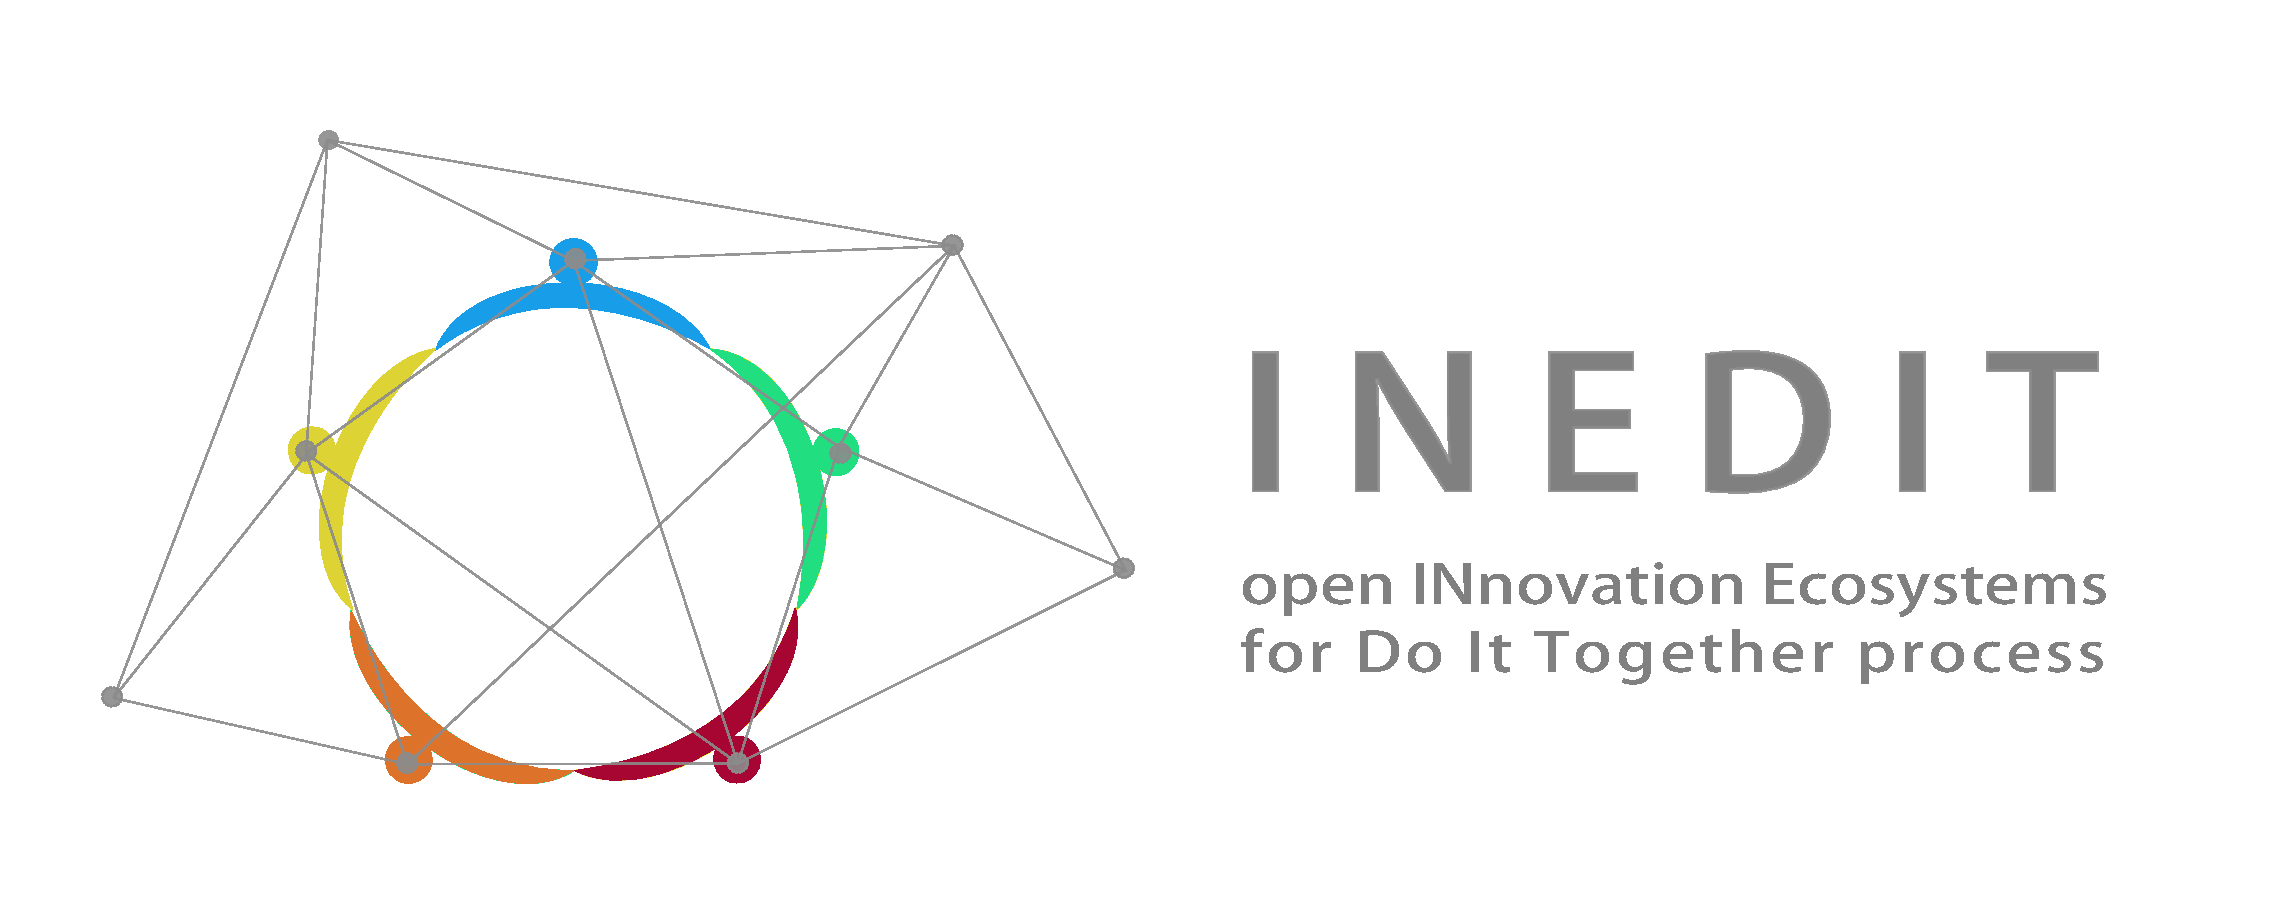
\includegraphics[width=\linewidth]{figures/Inedit_horiz.pdf}\\ 
		
		\vfill
		
		\textbf{\Huge{\textcolor{darkgray}{ D6.4 3D Printing of recycled plastic demonstrator }}} \\ 
		
		\vfill
		
		\vspace{60mm} 
		
		
		
      \textcolor{gray}{\rule{\textwidth}{2pt}}
      
		\vspace{5pt}
		\begin{tabular}{ c p{8cm} c }
           & & Version 3.0  \\ 
         WP6 T6.4  & & March 2023   \\ 
      \end{tabular}
		\vspace{5pt} 
		
		\textcolor{gray}{\rule{\textwidth}{2pt}}
		
		
	
		
		\vfill
		
	\end{center}
\end{titlepage}

\newpage



\begin{tabu} to \textwidth { X  X[0.7] | X | X }
\toprule


\multicolumn{2}{l |}{ \multirow{4}{*}{  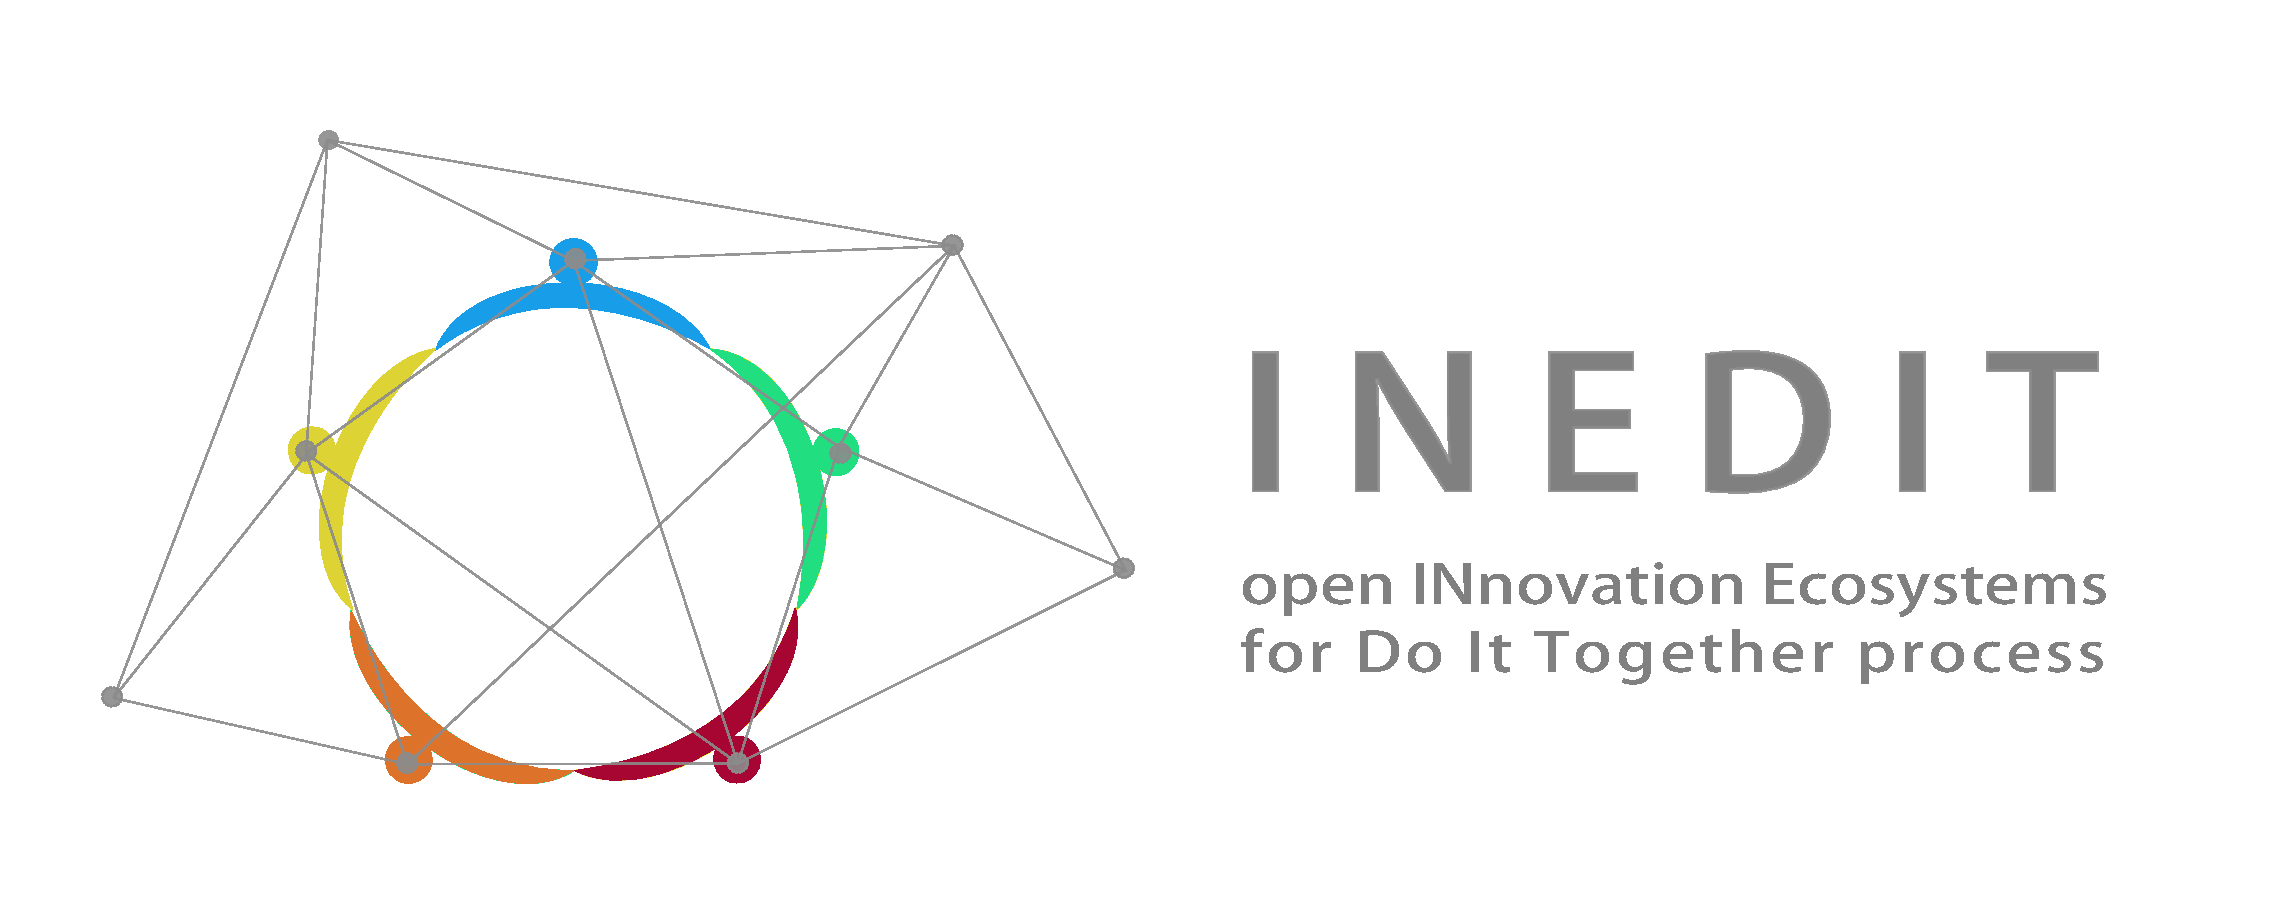
\includegraphics[width=7cm]{figures/Inedit_horiz.pdf} } }  & Work Package: & 6   \\ \cmidrule{3-4}
   & & Type of document:  & Deliverable        \\ \cmidrule{3-4}

   & & Due Delivery Date:    & January 31/2023     \\ \cmidrule{3-4}
 
   & & Actual Delivery Date:    & March 2023       \\ \midrule
 

\multicolumn{4}{l|}{ } \\ \midrule

 Responsible:    &  \multicolumn{3}{|l}{Université de Lorraine }        \\ \midrule
        
 Dissemination Level    &  \multicolumn{3}{|l}{ Public }  \\ \midrule
 Title:    &   \multicolumn{3}{|l}{ Report on the 3D printing of Recycled Plastic Demonstrator }    \\ \hline

 Description:    &    \multicolumn{3}{| p{\dimexpr0.75\linewidth-2\tabcolsep\relax}}{
Description of the conceptual framework of distributed recycling via additive manufacturing (DRAM) and its concrete implementation in a DIT approach. The technologies, materials and methods are reported. Several illustrative case studies are presented.
}   \\ \midrule
 
 
 \multicolumn{1}{l|}{Version}     &   \multicolumn{3}{|l}{ Version 3}    \\ \midrule
 \multicolumn{1}{l|}{Contributors}       & Versions    & Dates       & Revision Description \\ \midrule
\multicolumn{1}{l|}{WP6 Leader} & 0 & February 04/2023 & Validation of the global structure  \\ \midrule        
\multicolumn{1}{l|}{UL} & 1 & March 03/2022 & Revision of a version 1 \\ \midrule
\multicolumn{1}{l|}{UL and SCM} & 2 & March 17/2022 & Revision of a version 2 given the received comments \\ \midrule        
\end{tabu}


\vfill

\begin{center}
\textcolor{lightgray}{Disclaimer}

\textcolor{lightgray}{
\small
This document is provided « as is » with no warranties whatsoever, including any warranty or merchantability, non-infringement, fitness for any particular purpose, or any warranty otherwise arising out of any proposal, specification or sample.  No license, express or implied, by estoppels or otherwise, to any intellectual property rights are granted herein. The members of the project INEDIT do not accept any liability for actions or omissions of INEDIT members or third parties and disclaim any obligation to enforce the use of this document. }

\textcolor{lightgray}{
This document reflects only the authors' view and the Commission is not responsible for any use that may be made of the information it contains.  This document is subject to change without notice. 
}
\end{center}
\normalsize

\newpage

\ifdefined\Shaded\renewenvironment{Shaded}{\begin{tcolorbox}[frame hidden, boxrule=0pt, enhanced, interior hidden, breakable, borderline west={3pt}{0pt}{shadecolor}, sharp corners]}{\end{tcolorbox}}\fi

\renewcommand*\contentsname{Table of contents}
{
\hypersetup{linkcolor=}
\setcounter{tocdepth}{3}
\tableofcontents
}
\newpage

\bgroup
\hypersetup{linkcolor = black}
\listoffigures
\egroup

\color{darkgray}

\newpage

\hypertarget{executive-summary}{%
\section{Executive Summary}\label{executive-summary}}

This report describes the open manufacturing demonstration facility of
``\emph{3D printing of recycled plastic demonstrator}' developed in the
INEDIT project. The main goal is to validate the logistical and
technical feasibility of recycled assets to be used in the
Do-It-Together (DIT) approach. Therefore, a complete technical
description is presented to transform certain plastic wastes into
functional objects using 3D printing and desktop plastic injections
through multiple experimentations. The activities were oriented to
produce objects for the purpose of 1) manufacturing prototypes for
validation prior to production stage, 2) personalization of furniture
and 3) spare parts for reparability to enlarge the life of discarded
furniture.

These technical and logistical elements were implemented in a recycling
pilot platform known locally as the \emph{`Green FabLab'} at the city of
Nancy, France. The technical development was based on an open design
approach in order to be replicable to other countries. The integration
was validated according to Key Performance Indicators.

There are two majors outcomes of the work done within task 6.4 and
documented in this report:

\begin{enumerate}
\def\labelenumi{\arabic{enumi}.}
\tightlist
\item
  Describe the methodological concept of the distributed recycling via
  additive manufacturing (DRAM) system oriented to the revaluation of
  plastic.
\item
  Demonstrate in a relevant environment to prove the integration of a
  distributed and local plastic recycling with the INEDIT process.
\end{enumerate}

The development of open-source technologies that enable the main stages
for plastic recycling constitute a first chain validation. Moreover, the
implementation and development of Use Case 3 proved to validate the
technology maturity level from TRL4 to TRL6 and market readiness level
from MRL 1 to 3/4 for technologies used such as the smart collector and
fused granular fabrication. In addition, the creation of a local and
distributed plastic recycling chain at a territorial level constitutes
an important output for the impact of the project given the high level
objectives of INEDIT.

\hypertarget{outline}{%
\subsection{Outline}\label{outline}}

The report is structured into three main parts. The section
Section~\ref{sec-plastic} provides a baseline introduction regarding the
plastic recycling issues in European Union. Then, section
Section~\ref{sec-context} gives an overview of the context where the 3D
printing of recycled plastic demonstrator have been developed,
characterizing its main methodological and technical features. After,
the section Section~\ref{sec-dit} presents in detail the
operationalization of the demonstrator in the DIT approach. This is
illustrated the step-by-step technical elements to consider each element
and the illustrative experimentations made to validate each of the DIT
process. The rapport finish with a conclusion section.

\newpage

\hypertarget{introduction}{%
\section{Introduction}\label{introduction}}

INEDIT develops a multi-sided platform pursuing the goal of new
sustainable manufacturing processes integrated in agile manufacturing
networks to simplify personalization of furniture. To do that, a numeric
platform is devoted to connecting consumers, designers, makers, and
manufacturers in order to push further the access to production means
improving the creativity and design in open innovation ecosystems. This
trend is enframed in the concept of mass customization, identified as a
key major trend by the EU for 2030. In fact, the on-demand production
capacity (all around Europe) enabled by the DIT approach seeks to be
environmentally responsible.

The Université de Lorraine developed a pilot platform called locally as
the `Green Fablab' with the aim to describe and implement a 3D printing
of recycled plastic demonstrator. The ambition of this use case is to
test the feasibility of the distributed recycling via additive
manufacturing (DRAM) (\protect\hyperlink{ref-CruzSanchez2020}{Cruz
Sanchez et al., 2020}) concept with the purpose to integrate in the
Do-It-Together approach. The technical feasibility of the plastic
recycling via additive manufacturing was based on an open design
approach that could facilitate the replicability and appropriation in
different countries.

Therefore, the main goal of this task is to validate the logistical and
technical feasibility of recycled assets to be used in the DIT approach.
These technical and logistical elements were implemented in a relevant
environment. More precisely in a cultural and citizen third place at
Nancy, France.

The outputs of this use case aims to illustrate how the 3D printing of
recycled plastic demonstrator give a concrete results on the the
high-level objectives that the INEDIT project, namely:

\begin{itemize}
\tightlist
\item
  To unleash the creativity of consumers and designers towards
  co-creation of new pieces of furniture addressing the needs of the
  single user in an industrial context.
\item
  To democratize the access to production resources in the furniture
  sector.
\item
  To support SME operating in the furniture sector in finding new
  business opportunities.
\item
  To create a framework of solutions for creation, engineering and
  distributed production of customer driven pieces of furniture.
\item
  To define, design and manufacturing strategies focusing on lowering
  ecological impact and addressing societal challenges.
\item
  To create an ecosystem of all stakeholders within Europe.
\end{itemize}

\newpage

\hypertarget{sec-plastic}{%
\section{Plastic Issues for the European Union}\label{sec-plastic}}

Since 1950', our society has gained enormous advantages in terms of
quality of life thanks to the technical development of the development
of plastic and polymer materials. Plastic is a material that is widely
used in our daily lives and plays a fundamental role in industry and
economic development. The plastic material is found in almost all our
products: food packaging, cars, technological tools, clothing, among
others. The main reason is that plastic materials offer a variety of
chemical and mechanical properties to be useful for a wide array of
applications. Plastics are extremely useful, but their mismanagement has
affected the environment and our health. The over-consumption and
especially bad practices (single use, difficulty of reuse, etc.), make
plastics one of the major societal challenges of an ecological
transition that has become imperative. The main problem is the
end-of-life treatment which traditionally uses a centralized system
where plastic waste often has to travel thousands of kilometers\ldots{}
to be incinerated or landfilled. In addition to the energy and
environmental impact of their production, there is also the impact of
the end of life.

\begin{figure}[H]

{\centering 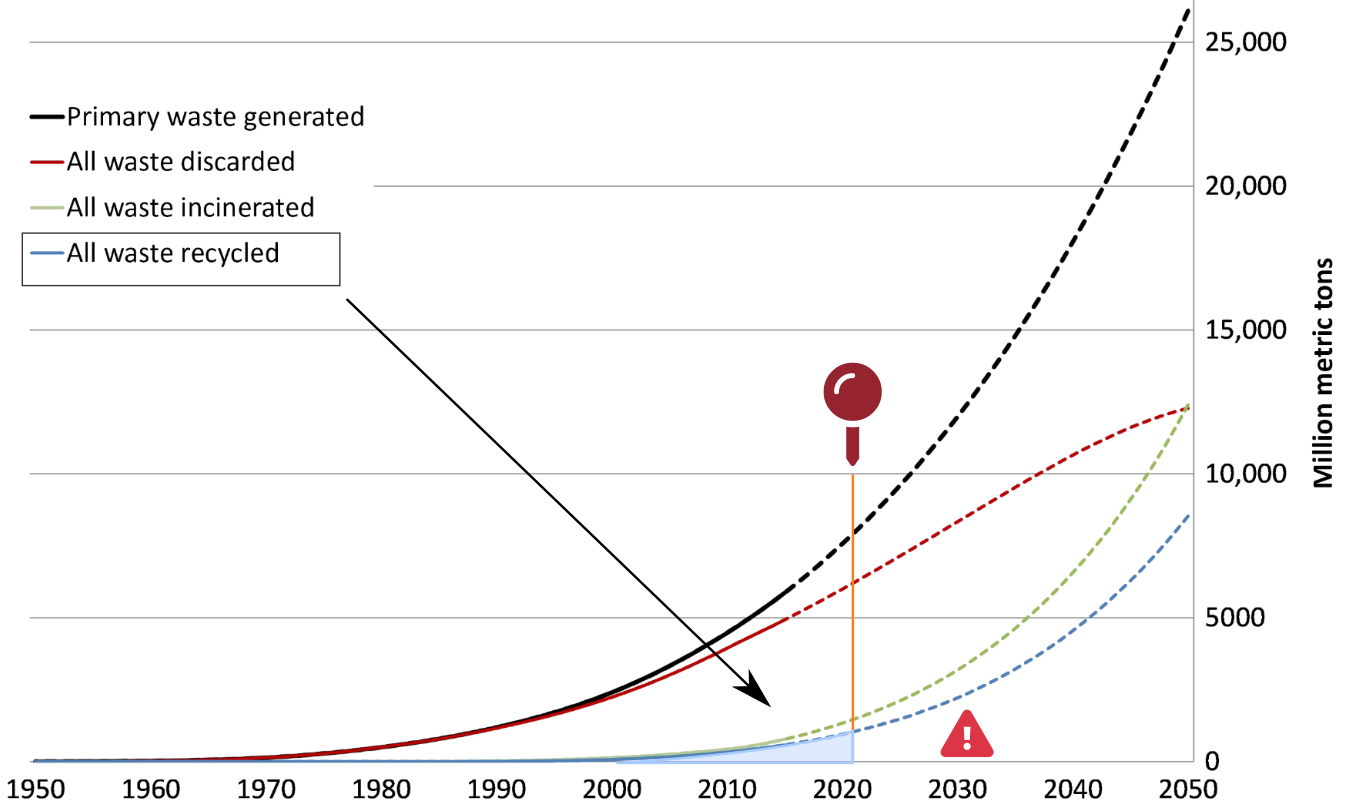
\includegraphics[width=0.65\textwidth,height=\textheight]{figures/Plastic-problem.png}

}

\caption{\label{fig-plastic-problem}Cumulative plastic waste generation
and disposal (in million metric tonnes). Source: adapted from Geyer et
al (2017)}

\end{figure}

Globally, only about 9\% of all plastics were recycled since 1950's up
to 2015 (\protect\hyperlink{ref-Geyer2017}{Geyer et al., 2017}) as
displayed by the Figure~\ref{fig-plastic-problem}. The share of plastic
in municipal solid waste (by mass) increased from less than 1\% in 1960
to more than 10\% by 2005 in middle- and high-income countries being a
packaging field, the largest market
(\protect\hyperlink{ref-Geyer2017}{Geyer et al., 2017}). Therefore,
single--used plastic materials are hardly recycled worldwide and
therefore they end up on the waste disposal sites, nature and oceans.
Over 300 million tons of plastic materials are annually produced
worldwide and from this amount, approximately 6300 Teragrams of plastic
waste had been generated considering estimations of 2015
(\protect\hyperlink{ref-Geyer2017}{Geyer et al., 2017};
\protect\hyperlink{ref-Wang2020a}{Wang et al., 2020}).

Unfortunately, the plastic waste pollution poses a major threat because
of the issue of non-degradability affecting the ecological environments
(\protect\hyperlink{ref-Hopewell2009}{Hopewell et al., 2009};
\protect\hyperlink{ref-Ryberg2019}{Ryberg et al., 2019};
\protect\hyperlink{ref-Thompson2009b}{Thompson et al., 2009}). Indeed,
recycling rates remain small (approx. 14\%) in the plastic packaging
field on a global scale
(\protect\hyperlink{ref-Hahladakis2018}{Hahladakis and Iacovidou,
2018}). Even in Europe, which tends to lead on environmental
stewardship, the recycling rate is about 32.5 wt\%
(\protect\hyperlink{ref-Plastics2019}{Plastics, 2019}). However, these
values consider the amount of plastic waste collected, rather than the
total amount in circulation
(\protect\hyperlink{ref-Kranzinger2018}{Kranzinger et al., 2018}).
Rethinking the development and use of plastics is central to the
circular economy paradigm, to provide less harmful options for the
environment. Thus, more types of plastic packaging are available, but
each reflects diverse circular economy strategies

Unfortunately, the plastic waste pollution poses a major threat because
of the issue of non-degradability affecting the ecological environments
(\protect\hyperlink{ref-Hopewell2009}{Hopewell et al., 2009};
\protect\hyperlink{ref-Ryberg2019}{Ryberg et al., 2019};
\protect\hyperlink{ref-Thompson2009b}{Thompson et al., 2009}). Indeed,
recycling rates remain small (approx. 14\%) in the plastic packaging
field on a global scale
(\protect\hyperlink{ref-Hahladakis2018}{Hahladakis and Iacovidou,
2018}). Even in Europe, which tends to lead on environmental
stewardship, the recycling rate is about 32.5 wt\%
(\protect\hyperlink{ref-Plastics2019}{Plastics, 2019}). However, these
values consider the amount of plastic waste collected, rather than the
total amount in circulation
(\protect\hyperlink{ref-Kranzinger2018}{Kranzinger et al., 2018}).
Rethinking the development and use of plastics is central to the
circular economy paradigm, to provide less harmful options for the
environment. Thus, more types of plastic packaging are available, but
each reflects diverse circular economy strategies

To tackle this accumulation waste problem, the European strategy for
plastics in the circular economy (CE) is gaining attention in the policy
and business debate surrounding sustainable development of industrial
production (\protect\hyperlink{ref-EC2018}{European Commission, 2018};
\protect\hyperlink{ref-Geissdoerfer2017}{Geissdoerfer et al., 2017}). CE
tackles a central societal issue concerning the current principle
``take, make, dispose'' (linear economy) and its negative effects caused
by the depletion of natural resources, waste generation, biodiversity
loss, pollution (water, air, soil) and non-sustainable economics
(\protect\hyperlink{ref-VanBuren2016}{van Buren et al., 2016}). The
validation (technical, economic, legislative) of waste plastic as a
secondary raw material in industrial processes is considered now a core
target to integrate CE into the plastic value chain
(\protect\hyperlink{ref-Simon2019}{Simon, 2019}). Strategies of open and
closed-loop recycling as well as upcycling and downcycling functionality
approaches can offer paths to validate the secondary raw materials
(\protect\hyperlink{ref-Zhuo2014}{Zhuo and Levendis, 2014}). The
promotion of cross-sectorial valorization of plastic wastes through
Industrial symbiosis approaches seems to be a relevant strategy for the
circular economy strategies of the EU
(\protect\hyperlink{ref-Karaylan2021}{Karayılan et al., 2021})

Based on this context, it is presented as a demonstration of the INEDIT
project called `3D Printing of Recycling Plastic' that was developed and
implemented.

\newpage

\hypertarget{sec-context}{%
\section{Context of the 3D Printing of Recycled Plastic
Demostrator}\label{sec-context}}

\hypertarget{presentation-of-the-scale-of-the-demonstrator-rives-de-meurthe-district-nancy-france}{%
\subsection{Presentation of the scale of the demonstrator: Rives de
Meurthe district (Nancy,
France)}\label{presentation-of-the-scale-of-the-demonstrator-rives-de-meurthe-district-nancy-france}}

The demonstrator is placed at the City of Nancy - France, in the region
of Lorraine at the northeastern. Nancy is the capital of the
Meurthe-et-Moselle department and has a population of approximately
105,000 inhabitants. More precisely, our interest is the \emph{Rives de
Meurthe} district as presented by the Figure~\ref{fig-rives}. This
district extends between the city center and the Meurthe River for about
7 km from north to south (extending into the municipalities of
Jarville-la-Malgrange upstream and Maxéville downstream) and is between
250 and 1,000 m wide.

\begin{figure}

\begin{minipage}[t]{0.47\linewidth}

{\centering 

\raisebox{-\height}{

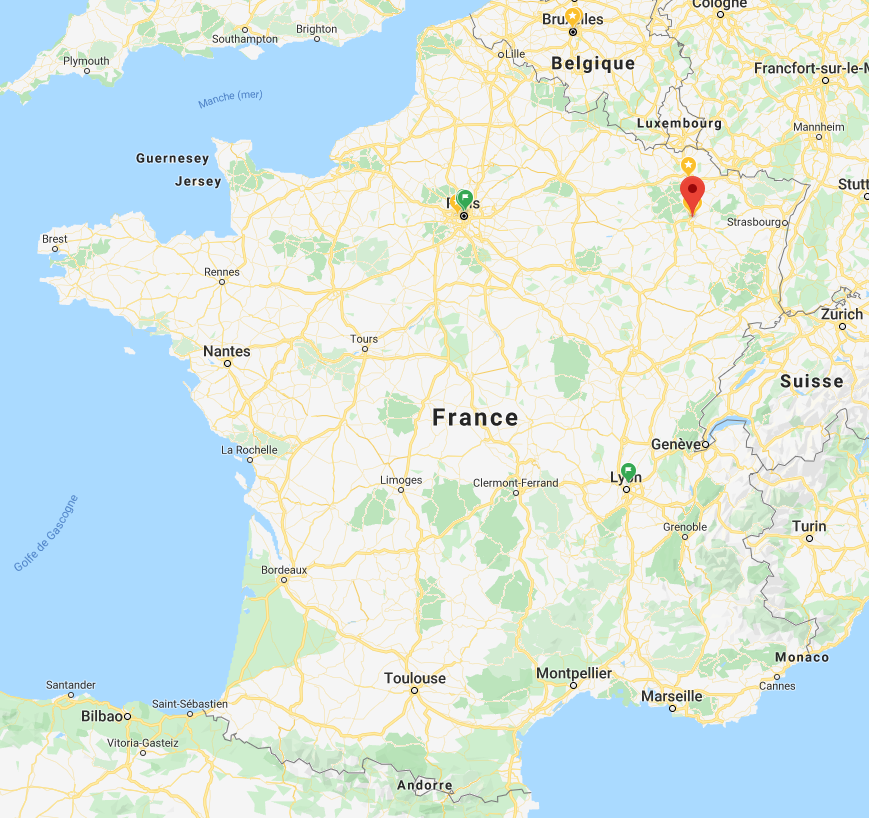
\includegraphics{figures/Nancy-00.png}

}

}

\end{minipage}%
%
\begin{minipage}[t]{0.06\linewidth}

{\centering 

~

}

\end{minipage}%
%
\begin{minipage}[t]{0.47\linewidth}

{\centering 

\raisebox{-\height}{

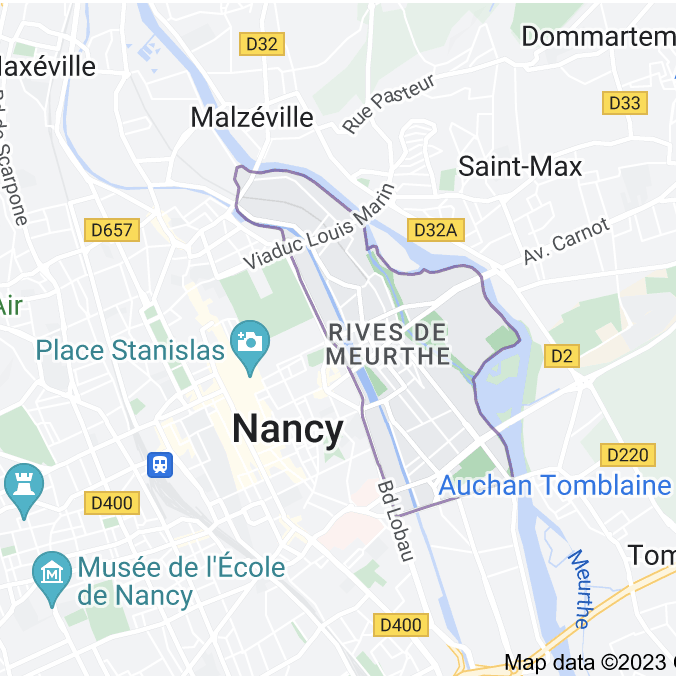
\includegraphics{figures/ok3/Rives-of-meurthe.png}

}

}

\end{minipage}%

\caption{\label{fig-rives}Localization of the Rives the Meurthe district
at Nancy, France.}

\end{figure}

Nancy was not born around a waterway and its commercial potential. Its
port and river side has long been rather reduced, contrary to the great
majority of cities. However, the main interest of the Rives de Meurthe
district concerns that it has been a case study in the light of urban
regeneration due to flood risk presented in this area
(\protect\hyperlink{ref-chiffre2014}{Chiffre et al., 2014};
\protect\hyperlink{ref-edelblutte2006}{Edelblutte, 2006}). Therefore,
since the end of 1980's, there have been a series of renewal policies of
the district with the purpose of going beyond a simple reconversion by
broadly rethinking the role of the central and peri-central space of the
city.

Among the multiple choices, one of the strategic actions taken by the
government has been the transformation of the old site of the
slaughterhouses in the heart of the Rives de Meurthe district. In 1996,
the slaughterhouse activity was transferred to the Épinal-Mirecourt ZAC,
marking the end of the site's industrial life. As soon as the activities
ceased, a rehabilitation process began in parallel with the development
project of the district. The vast 6-hectare site was first carefully
demolished to bring back the main buildings constructed at the beginning
of the 20th century.

In 2017, the city administration took the decision by a public
consultation to create exemplary actions in terms of ecological
transition at the city level
(\protect\hyperlink{ref-villedenancy2018}{Ville de Nancy, 2018}). Thus,
the creation on the site of the former slaughterhouses was taken. This
gives birth in 2019 to the creation of the OK3 association to develop
and animate the cultural project of \emph{L'Octroi Nancy} towards the
creation of a Cultural and Creative Incubator.\footnote{See more details
  in https://www.octroi-nancy.fr/}

Given the pandemic situation at the beginning on 2020, the end of works
was only finished in 2021.

\hypertarget{third-place-octroi-nancy}{%
\subsection{Third place Octroi Nancy}\label{third-place-octroi-nancy}}

The third place Octroi Nancy is an urban project that transforms the
former slaughterhouses of the city of Nancy into \emph{``cultural,
creative and citizen''} third place with 4600 \(m^2\) of renovated
buildings.

Four large buildings (Figure~\ref{fig-ok1}) were refurbished to provide
a convivial and multidisciplinary meeting place between culture and
innovation; open to experimentation and intended to operate as a
creative laboratory for the city. The first building (1) are called the
`La Petite Halle' (\emph{The Small Hall}) which is a space of 900
\(m^2\). The purpose is to develop a creative laboratory from which
projects of all artistic and creative disciplines may emerge. The second
building (2) is the `L'Octroi Sud' (\emph{South Octroi}) where it is
intended the professionalization for the actors of the territory,
through the installation of resource organizations. The third building
(3) is the `La Grande Halle' (\emph{The big Hall}). It is a hangar
building of 2,200 \(m^2\) space for the organization of events,
exhibitions and demonstration of artistic and cultural projects.
Finally, the fourth building (4) is the `La Halle ouverte' (\emph{the
Open Hall}) which is an open space of 700 \(m^2\) to host in particular
a weekly organic market and several intermittent cultural activities
mostly in the summer holidays.

\begin{figure}[H]

{\centering 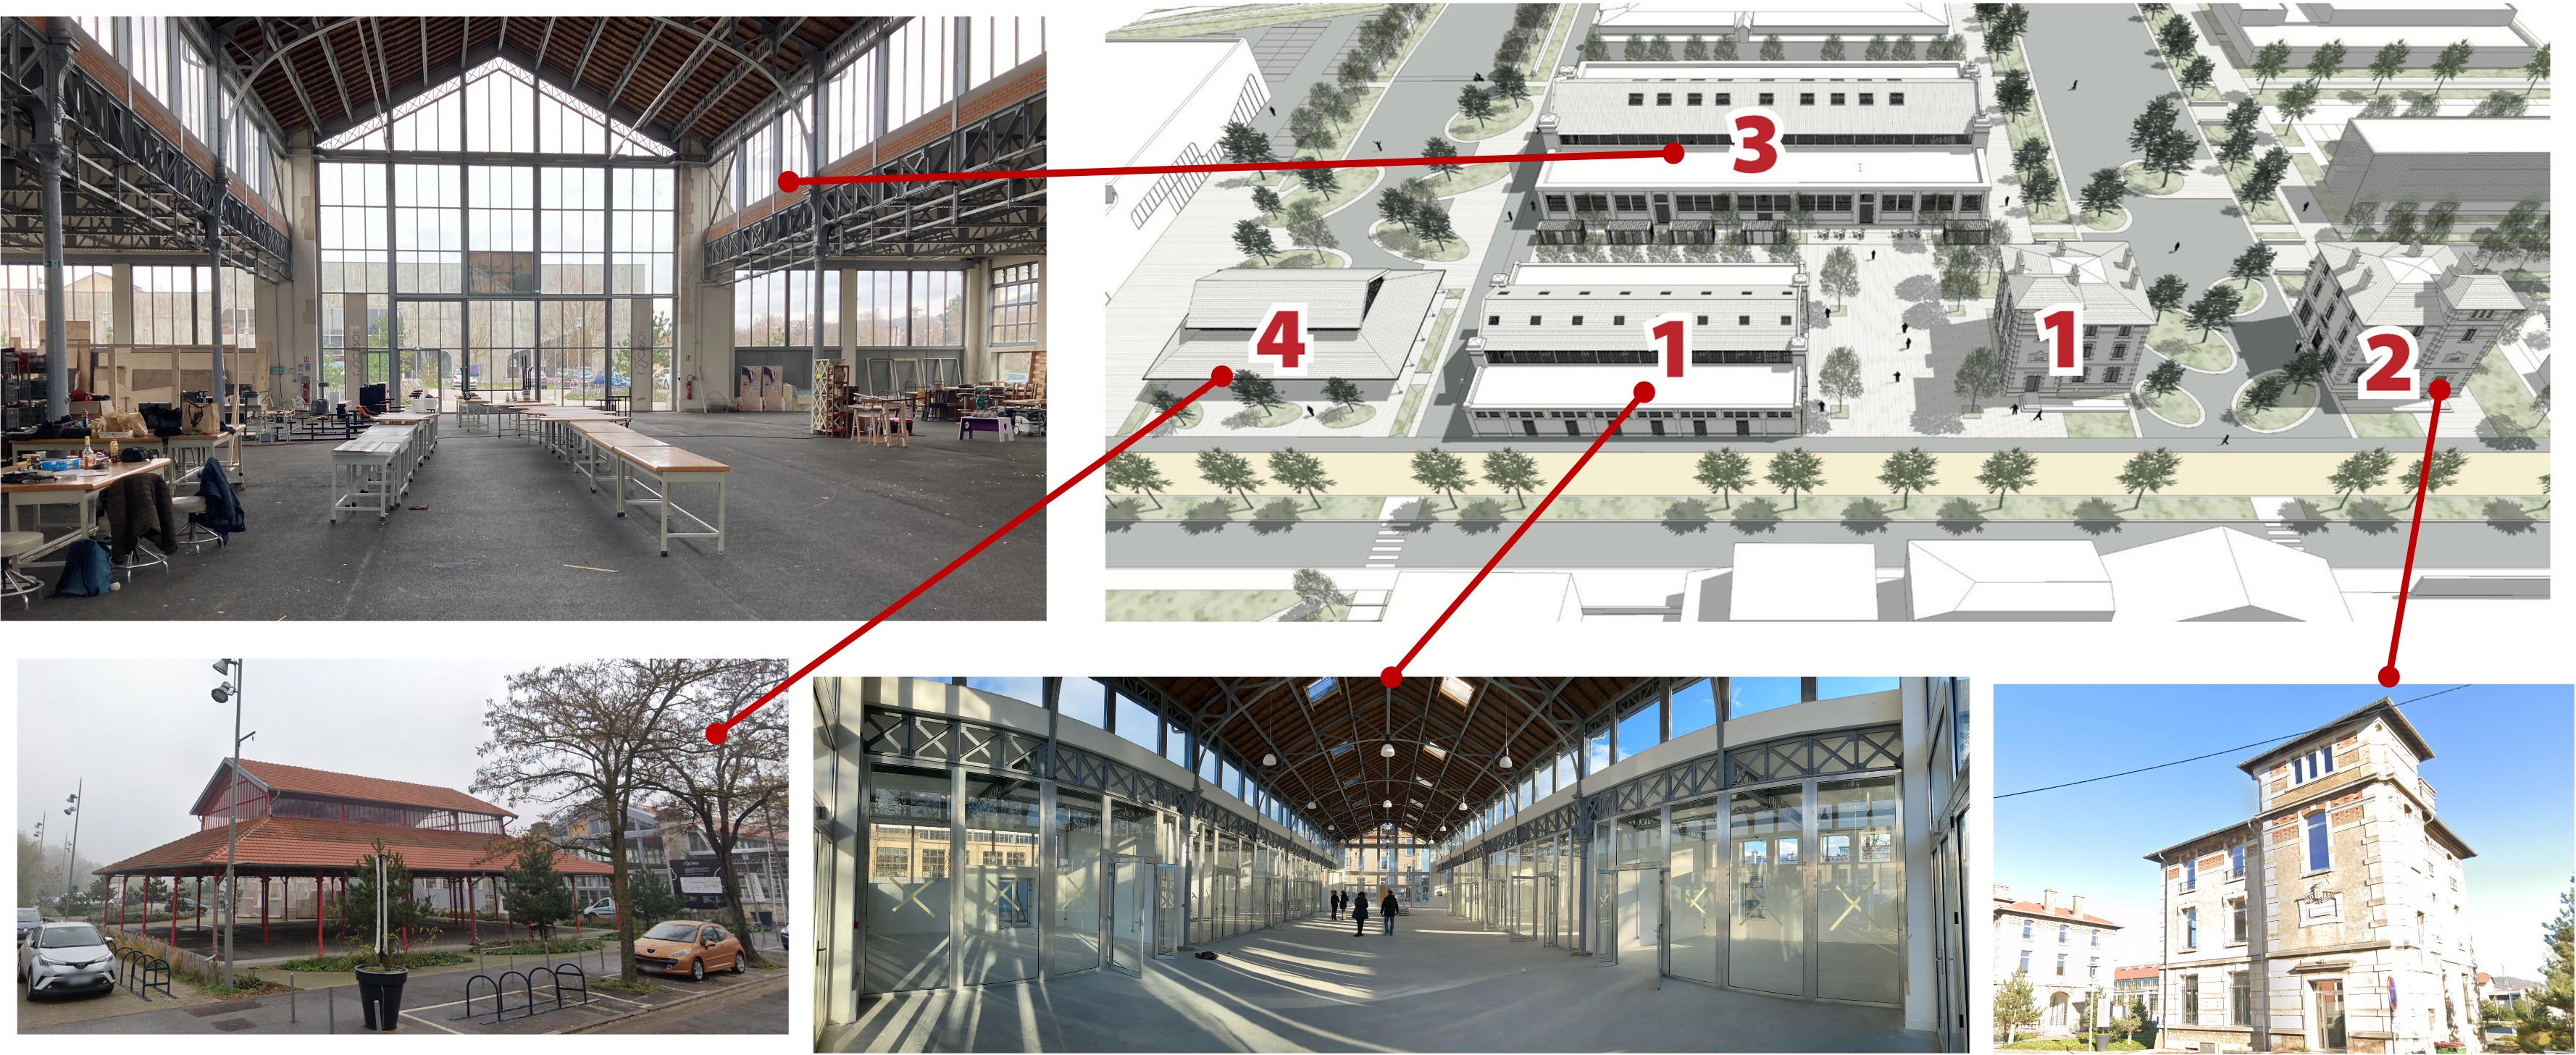
\includegraphics[width=0.9\textwidth,height=\textheight]{figures/ok3/OK3-01.jpg}

}

\caption{\label{fig-ok1}Overview of the Octroi facilities at the Rives
of Meurthe district}

\end{figure}

In summary, these types of third places are open ecosystems that will
bring together artists, researchers and creative people with the public,
the city's inhabitants and businesses. These initiatives can be framed
as socio-technical imaginary projects with new goals and desirable urban
transitions in Europe (\protect\hyperlink{ref-Fratini2019}{Fratini et
al., 2019}). Starting from existing facilities, this type of urban
initiatives can give an opportunity for socially inclusive and
environmentally responsible new roles of the local actors regarding the
city development.

\hypertarget{lorraine-fab-living-lab}{%
\subsection{\texorpdfstring{Lorraine Fab Living
Lab\textregistered}{Lorraine Fab Living Lab}}\label{lorraine-fab-living-lab}}

Connected to the Octroi ecosystem, the \textbf{Lorraine Smart Cities
Living Lab (LSCLL)} is a trans-disciplinary resource center of the
Université de Lorraine. It aims to support and link the different
societal challenges of the Lorraine territory with the local resources.
It enables the integration of different users, implementing
collaborative and agile approaches in the service of \emph{Research,
Development of Innovations, Training and a Citizen Culture}. Since 2010,
this initiative is a member of the European Network of Living Labs
(ENoLL)\footnote{4\(^{th}\) wave of labellisation}, seeking to develop
public-private-population partnerships (PPPPs) to disseminate innovation
and related practices.

Since 2014, the LSCLL formalizes its strategic intention with the
Lorraine Fab Living Lab\textregistered (LF2L\textregistered) research
platform for prospective assessment of innovative usages
(\protect\hyperlink{ref-Dupont2016}{Dupont et al., 2016}).

The LF2L physical environment is constituted by a collaborative and a
fablab space. The collaborative space allows users to foster cooperation
in engineering design with different stakeholders in order to create new
concepts/designs. On the other hand, the fablab space allows users to
materialize the concepts/designs in an easy and quick way in order to
have a prospective evaluation (\protect\hyperlink{ref-Boujut2003}{Boujut
and Blanco, 2003}; \protect\hyperlink{ref-Dupont2015b}{Dupont et al.,
2015}, \protect\hyperlink{ref-Dupont2014}{2014}). The synergy of these
two spaces enables the project development in a living lab approach
taking into account the user centered design principles. The conceptual
framework is composed of three main elements as illustrated in
Figure~\ref{fig-lf2l-methodology}:

\begin{figure}[H]

{\centering 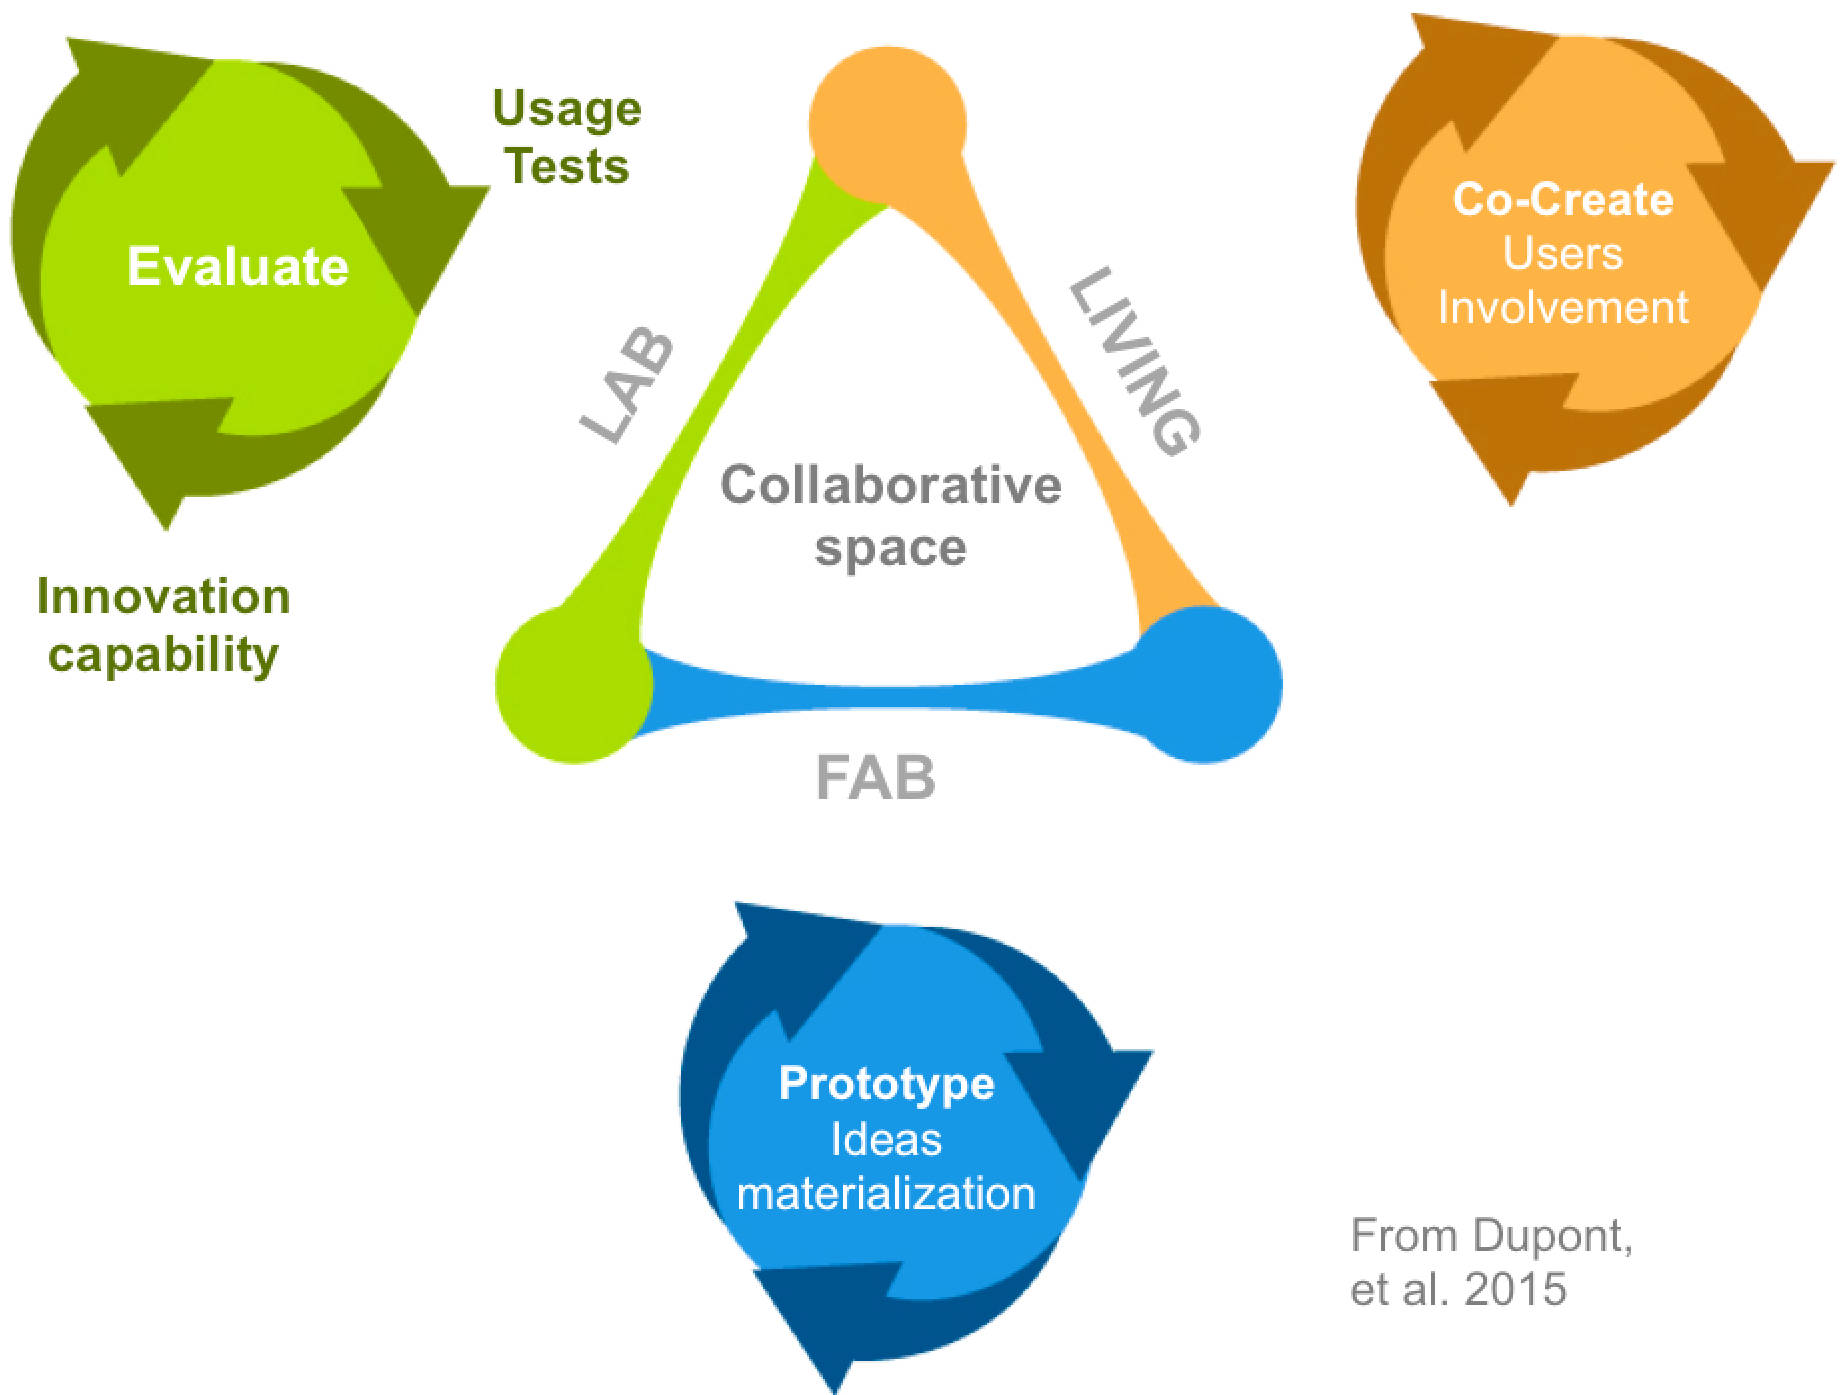
\includegraphics[width=3.125in,height=\textheight]{figures/lf2l/Methodology-01.jpg}

}

\caption{\label{fig-lf2l-methodology}The Lorraine Fab Living Lab
methodology.}

\end{figure}

\begin{enumerate}
\def\labelenumi{\arabic{enumi}.}
\tightlist
\item
  \emph{Co-creation}: Creative process to find alternative resolution
  concepts to a problem-topic given integrating the key stakeholders in
  the process.
\item
  \emph{Prototyping}: Materialization (virtual/real) of the concept in
  order to have a first and quick in- sight.
\item
  \emph{Evaluation}: Establishment of the pertinence of the concepts in
  order to create a feedback/improvement process.
\end{enumerate}

The conceptual innovation framework of LF2L takes into consideration the
2D (concept), 3D (object), 4D (over time) approaches involving different
type of stakeholders (e.g.~researches, companies, networks,) in order to
have a foresight usage evaluation of a new concept, technology or
project. The stages and 2D/3D/4D resources allow prospective assessment
of innovative usages in order to support this conceptual framework
inside this ``innovation space'' as indicated in figure 2.3
(\protect\hyperlink{ref-Dupont2016}{Dupont et al., 2016},
\protect\hyperlink{ref-Dupont2015b}{2015}). This approach is useful to
accelerate the deployment of industrial and/or urban demonstrators.

\newpage

\hypertarget{d-printing-of-recycled-plastic-demonstrator-the-green-fablab}{%
\section{3D Printing of recycled plastic demonstrator: the ``Green
FabLab''}\label{d-printing-of-recycled-plastic-demonstrator-the-green-fablab}}

\hypertarget{rationale-for-the-technological-system-of-the-3d-printing-recycling-demonstrator}{%
\subsection{Rationale for the technological system of the 3D printing
recycling
demonstrator}\label{rationale-for-the-technological-system-of-the-3d-printing-recycling-demonstrator}}

The main goal of the 3D Printing of Recycled Plastic Demonstrator, also
known locally as the `\emph{Green Fablab}' as illustrated in the
Figure~\ref{fig-gf-2021}, is to validate the logistical and technical
feasibility of recycled assets to be used in the DIT approach. The
logistical and technical aspects were implemented in a relevant
environment in order to prove the integration of a distributed and local
plastic recycling chain as a Open Manufacturing Demonstration Facilities
(OMDF). The \emph{Green Fablab} is the recycling pilot platform based on
an open design approach with the purpose to be replicable to other
countries. The results of this experimentation can be a baseline for
many archetypes of open communities such as fablabs, hackerspaces or
even industrial prototyping zones. This socio-technical demonstrator
combines the hardware development of distributed recycling with a living
lab approach that a citizen third place ecosystem can foster.\\
The different key performance indicators were established and validated.

\begin{figure}[H]

{\centering 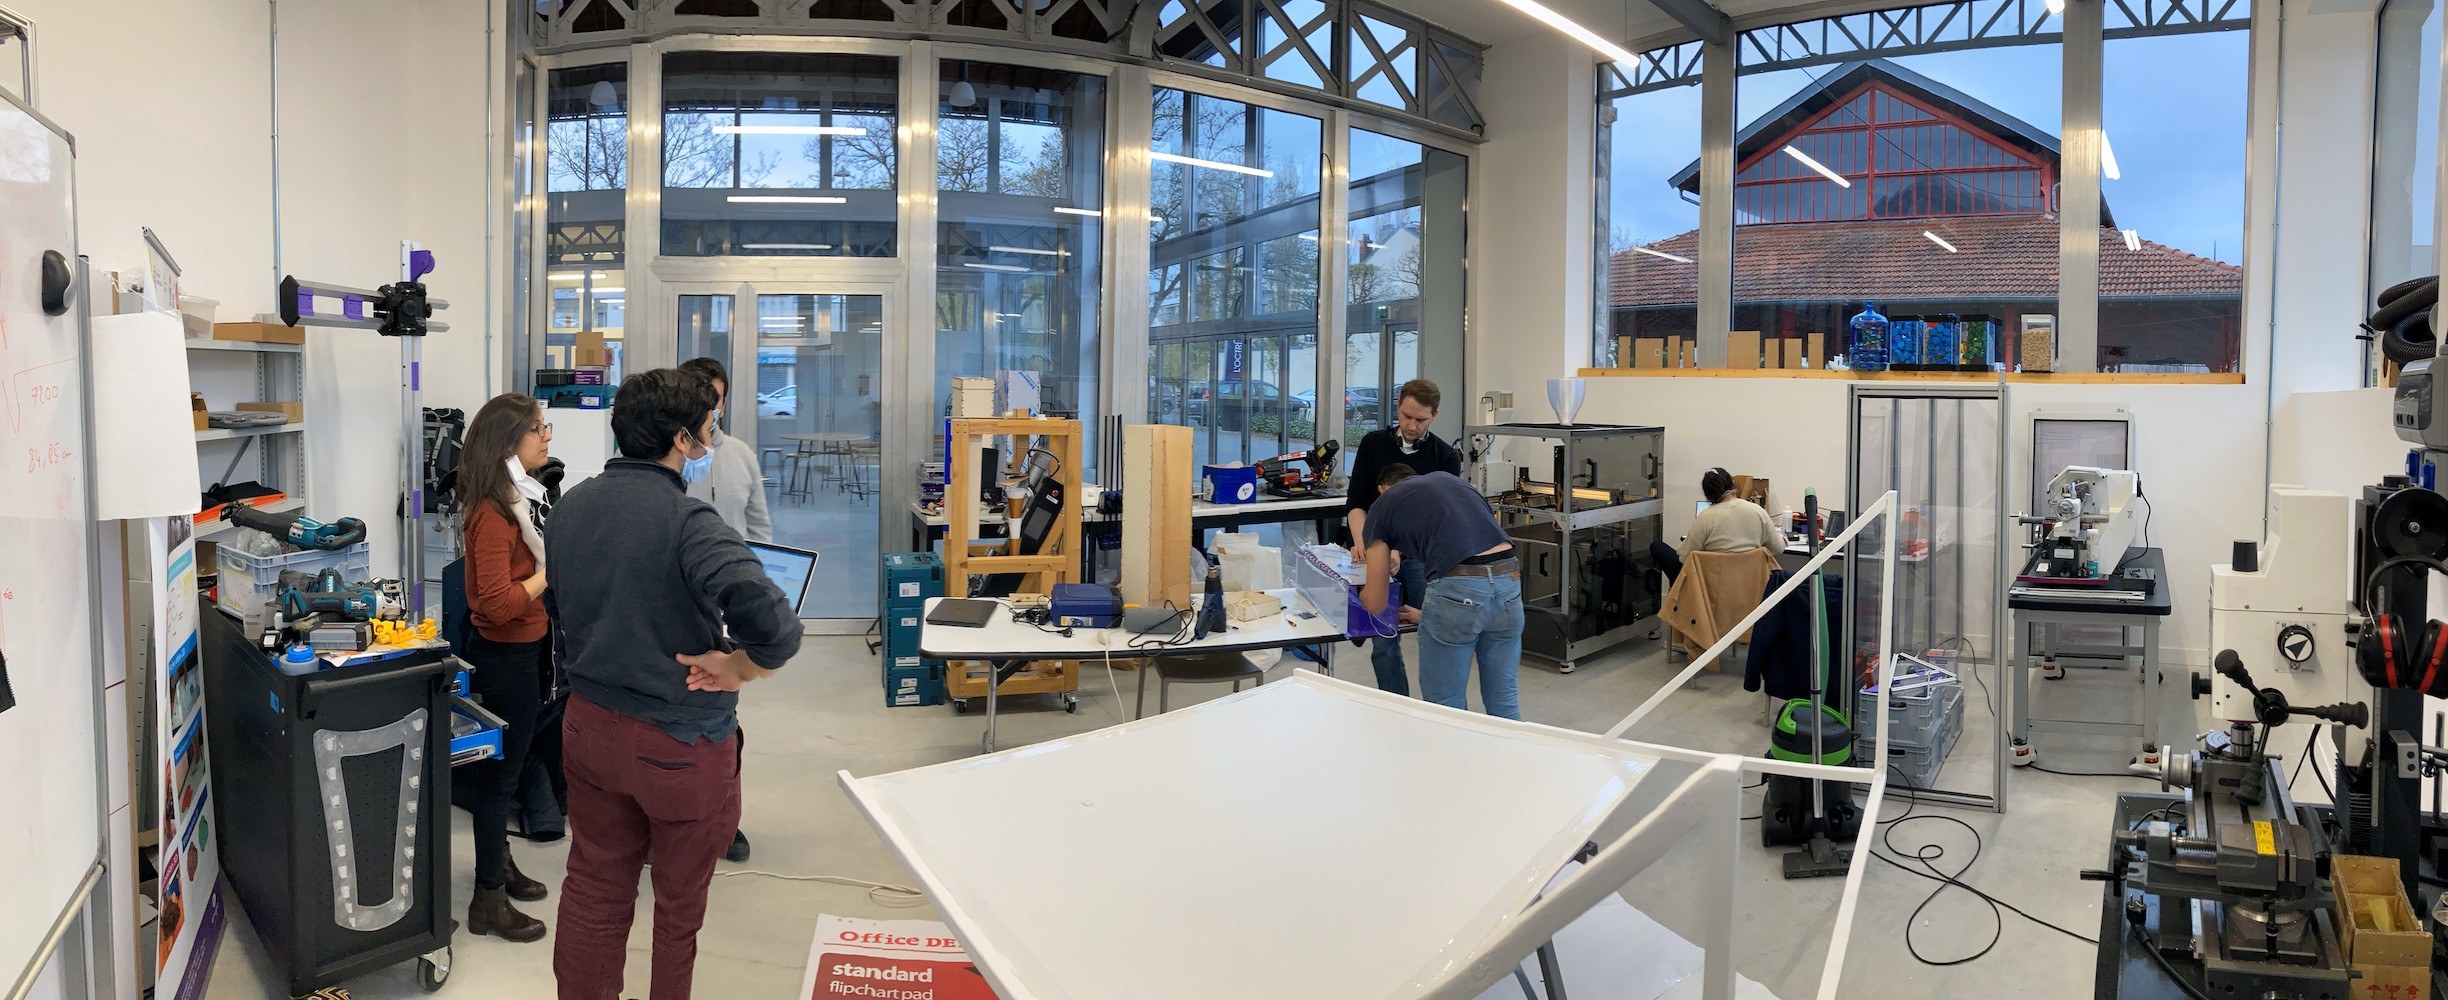
\includegraphics[width=0.9\textwidth,height=\textheight]{figures/2021-11-17-octroi.jpeg}

}

\caption{\label{fig-gf-2021}Initial overview of the Green Fablab at
November 2021}

\end{figure}

Initially, the initial technical equipment of the Green fablab was first
incubated at the facilities of the LF2L building. This was part of a
consolidation of previous research works
(\protect\hyperlink{ref-sanchez2016}{Sanchez, 2016}). After the Covid
Pandemic situation and the refurbishing that were made at the Octroi
ecosystem, the Green Fablab was installed only in November 2021.

One of the main ambitions of this demonstrator in the INEDIT project is
\textbf{to prove that plastic waste material can have several uses, and
therefore several values, during its life cycle}. The same material
could be recycled and transformed into new raw material for different
products. It is in this spirit that many associations, SMEs, local
authorities and individuals are developing new local recycling practices
that could allow us to aim for an economy that is more respectful of the
environment, fairer for society and more engaging for local politicians.

Therefore, it was imperative to understand the key conditions under
which to deploy a notion of circular economy with plastic waste to
possibly establish a secondary raw material market. Likewise, it was
required the study of technical parameters for the technological
diversity to possibly use the waste material including the open source
3D printers and manual desktop injection. The outputs are, not only by
minimizing use of the environment as a sink for residuals but -- perhaps
more importantly -- by minimizing the use of virgin materials. Hence,
the environmental impact of this technology is significantly reduced.

\hypertarget{distributed-recycling-via-additive-manufacturing-dram}{%
\subsection{Distributed recycling via Additive Manufacturing
DRAM}\label{distributed-recycling-via-additive-manufacturing-dram}}

The technical development of Green Fablab demonstrator is based on the
\textbf{distributed recycling via additive manufacturing (DRAM) approach
(\protect\hyperlink{ref-CruzSanchez2020}{Cruz Sanchez et al., 2020}).
This conceptual framework is a major scientific output from the INEDIT
project as a proposition of the future industrial landscape}.

The Additive manufacturing (AM) technology -also known as 3D printing-
which is an important industrial vector given its direct (and
distributed) manufacturing capabilities. This set of technologies are
becoming a key industrial process that could play a relevant role in the
transition from a linear to circular economy
(\protect\hyperlink{ref-Despeisse2016}{Despeisse et al., 2017}). AM
technologies is expected to transform the production process
(\protect\hyperlink{ref-Chen2017}{Chen et al., 2017};
\protect\hyperlink{ref-Jiang2017}{Jiang et al., 2017};
\protect\hyperlink{ref-Rahman2018}{Rahman et al., 2018}) thanks to its
ability to transform a numerical model into a deposition of material
(points, lines or areas) to create a 3D part
(\protect\hyperlink{ref-Bourell2017}{Bourell et al., 2017}). The
expiration of the first patents has contributed to an increased
interest, creating consumer value and potential for disruption
(\protect\hyperlink{ref-Beltagui2020}{Beltagui et al., 2021};
\protect\hyperlink{ref-West2016a}{West and Kuk, 2016}). In economic
terms, the global additive manufacturing market is expected to reach USD
23.33 billion by 2026 (\protect\hyperlink{ref-ReportsAndData2019}{Data,
2019}). However, determining when and how to take advantage of the
benefits is a challenge for traditional means of production. From a
societal viewpoint, Jiang et al.
(\protect\hyperlink{ref-Jiang2017}{2017}) reported that the product
development could change from traditional stage-gate models to
iterative, agile processes changing the scenario by 2030.

DRAM is defined as the use of recycled materials by means of mechanical
recycling process in the 3D printing process chain. In the literature,
the DRAM approach emphasizes the technical steps required to reuse
plastic waste through the recycling chains for material-extrusion-based
3D printing (\protect\hyperlink{ref-CruzSanchez2020}{Cruz Sanchez et
al., 2020}; \protect\hyperlink{ref-Little2020}{Little et al., 2020}).
The use of recycled material, either in the form of raw material or
blended with virgin material, is a method of special interest to
contribute to sustainable manufacturing
(\protect\hyperlink{ref-Zhao2018}{Zhao et al., 2018}).\\
Figure~\ref{fig-dram} illustrates the conceptual model of DRAM.

\begin{figure}[H]

{\centering 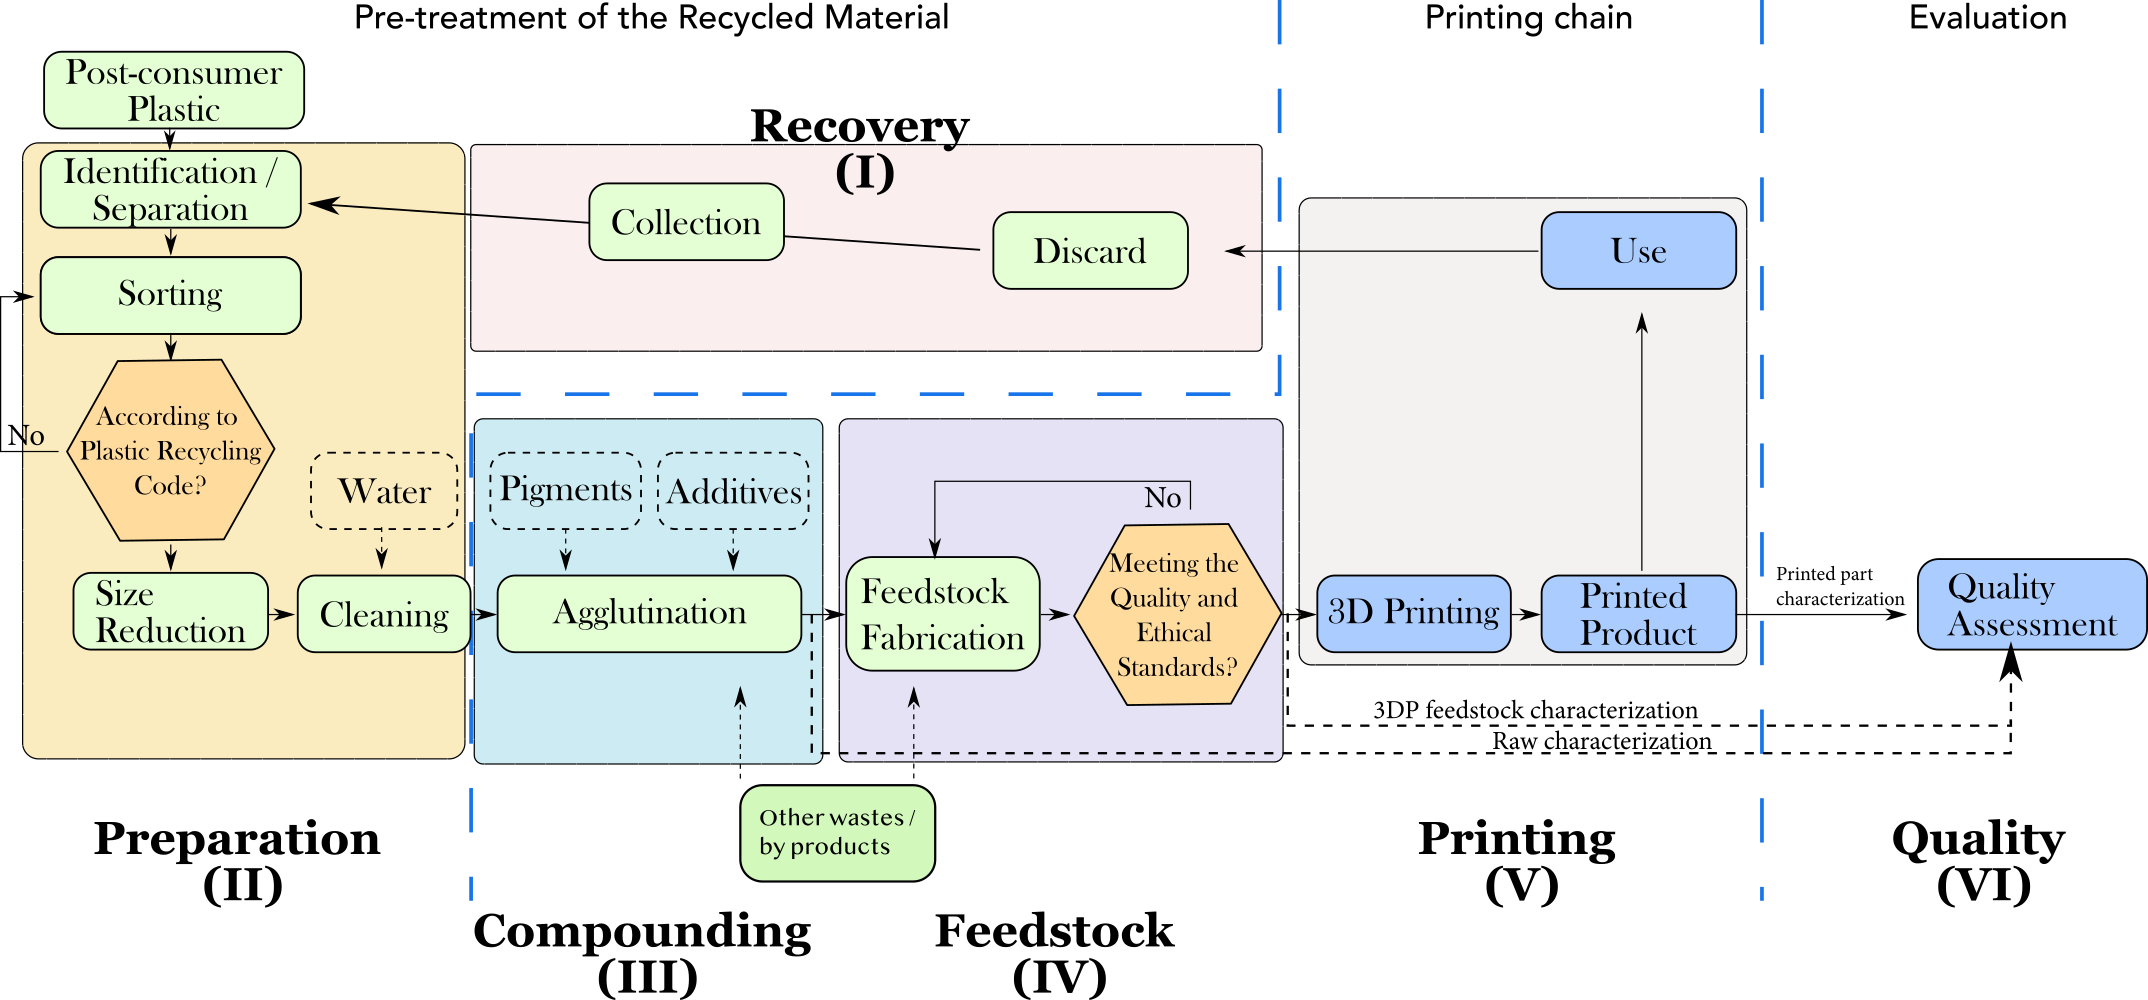
\includegraphics[width=0.9\textwidth,height=\textheight]{figures/DRAM-10.png}

}

\caption{\label{fig-dram}Distributed recycling via additive
manufacturing (DRAM) approach
(\protect\hyperlink{ref-CruzSanchez2020}{Cruz Sanchez et al., 2020})}

\end{figure}

In a general overview, the \textbf{Recovery (I)} phase concerns the
logistic operations to consider to collect the plastic wastes to be
reused in DRAM. The \textbf{Preparation (II)} phase corresponds to the
actions and strategies to identify, separate, sort, size reduce and
clean waste plastic to guarantee adequate quality for DRAM. The
\textbf{Compounding (III)} phase refers to the development of mono- and
composite-materials. The \textbf{Feedstock (IV)} phase identifies the
actions to fabricate the material usable for the printing process,
either filament for Fused Filament Fabrication (FFF) or the particle
size for Fused Granular Fabrication (FGF). The \textbf{Printing (V)}
stage identifies applications and process improvements for the recycled
printed part. The \textbf{Quality (VI)} phase identifies the multi-level
technical characterization performed to the recycled material.

The distributed manufacturing/recycling approach enables an alternative
option from an economy-of-scale to an economy-of-scope, where the
products are highly personalized satisfying niche communities or even
individuals (\protect\hyperlink{ref-Hienerth2014}{Hienerth et al.,
2014}). For these reasons, the AM technology could be a driver for a
shift in manufacturing from globally distributed production to local
facilities. Significant efforts are being made by industry and the
scientific community to move AM techniques from rapid prototyping and
tooling stages towards direct digital manufacturing (DDM)
(\protect\hyperlink{ref-Mueller2012}{Gibson et al., 2010};
\protect\hyperlink{ref-Holmstrom2016}{Holmström et al., 2016}), with the
concomitant environmental and social benefits. Nevertheless, Niaki et
al. (\protect\hyperlink{ref-Niaki2019}{2019}) demonstrated that
environmental and social benefits are not the key preferential factors
in the adoption of AM technologies in different industrial sectors. Only
the economic factor remains relevant in the AM implementation,
considering time- and cost-saving as the most important reasons.

\hypertarget{positioning-of-use-case-in-the-dit-approach.}{%
\subsection{Positioning of Use case in the DIT
approach.}\label{positioning-of-use-case-in-the-dit-approach.}}

Regarding the structuration of the INEDIT project\footnote{Delivrable
  2.2 DIT DESIGN OF THE DIT APPROACH AND XD FRAMEWORK}, the 3D printing
of recycled plastic demonstrator is positioned in certain stages of the
INEDIT approach as presented in the figure Figure~\ref{fig-dit-ul}.

\begin{figure}[H]

{\centering 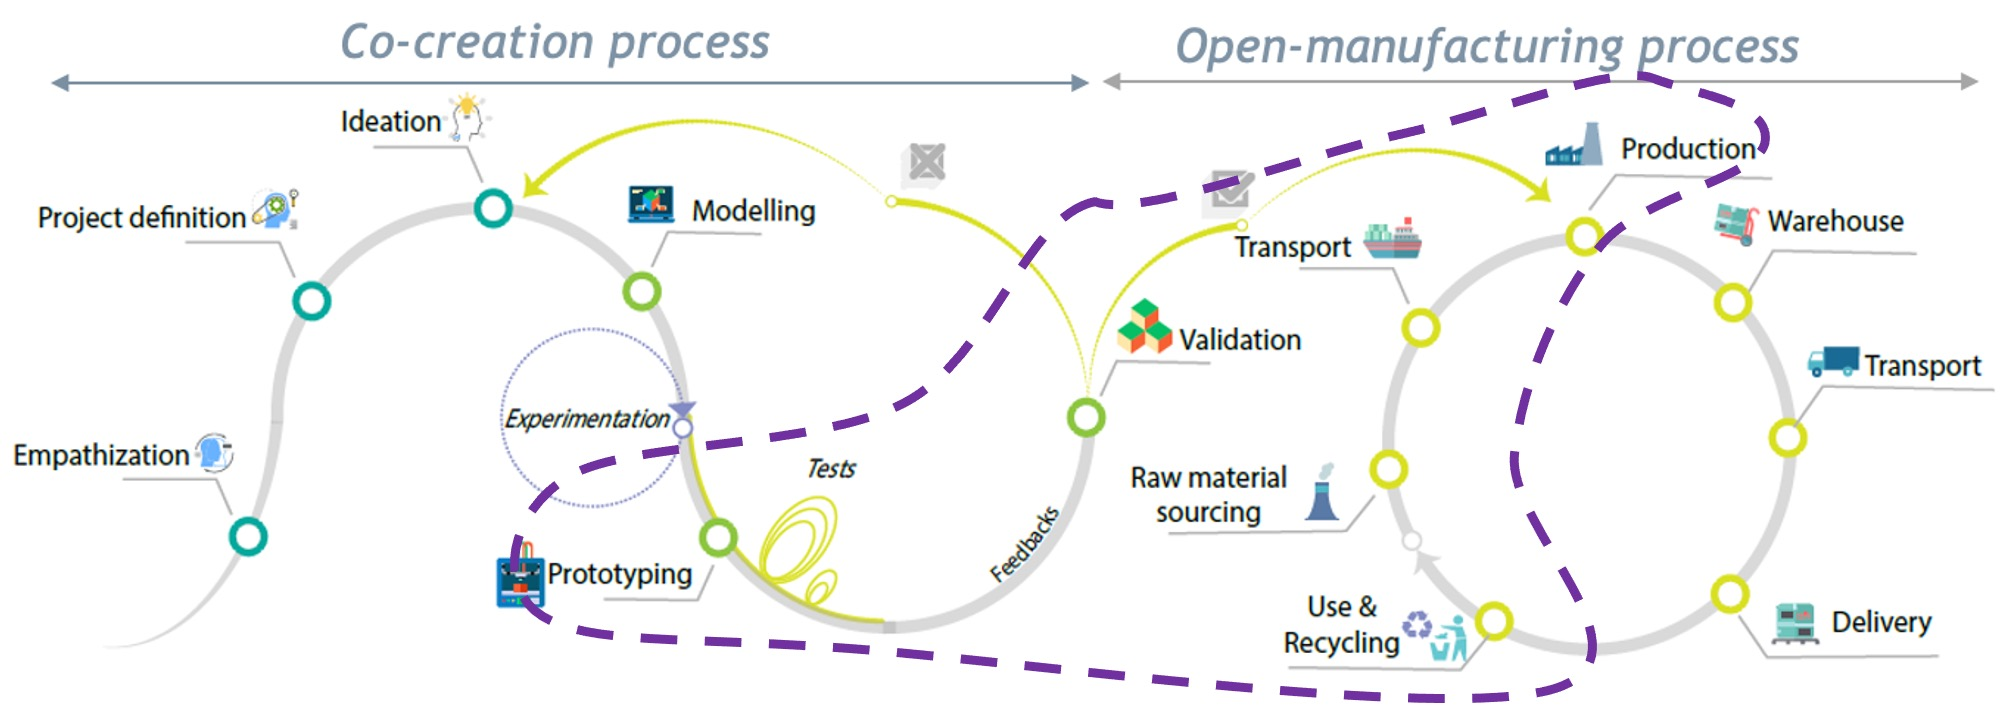
\includegraphics[width=0.9\textwidth,height=\textheight]{figures/DIT-UL.jpg}

}

\caption{\label{fig-dit-ul}Connection of the 3D printing Recycled
Plastic demonstrator in the Do-It-Together approach of INEDIT}

\end{figure}

In the co-creation phase, the use case deals with the prototyping aspect
of the possible furniture. On the other hand, in the open-manufacturing
process, our use case deals mainly with the raw material sourcing,
production and recycling aspect. These outputs are linked with a
validation stage.

In the following lines, we explain the assumptions made in the
deployment of the demonstrator and the technical characterization of
each phase. The technical characterization entails the technologies
mobilized.

\hypertarget{hypothesis-of-ul-case-for-deployment-in-reality}{%
\subsection{Hypothesis of UL case for deployment in
reality}\label{hypothesis-of-ul-case-for-deployment-in-reality}}

The implementation of the Green Fablab needs to be done considering
certain assumptions and simplifications to reduce the complexity of this
socio-technical system. The following assumptions were assumed in terms
of geographical scale, material recollection and manufacturing aspects:

\begin{itemize}
\item
  From a material perspective, only certain types of plastic wastes are
  considered. Specifically, Polyethylene terephthalate (PET), High
  density Polyethylene (HDPE), Polypropylene (PP) and Polylactic Acid
  (PLA). The major reason is from the technical perspective relies on
  the availability of these materials at the local area around the
  physical demonstrator.

  \begin{itemize}
  \tightlist
  \item
    PLA is one of the most used plastics in 3D printing. Thus, as a
    plastic waste source, PLA waste can be found from printed prototypes
    or 3D printed parts discarded.
  \item
    HDPE is a thermoplastic widely used in packaging.\\
  \item
    PET is the main material of water bottles in the market.
  \end{itemize}
\item
  The sorting, separation and cleaning process of plastics wastes are
  critical processes of recycling. Therefore, to make technical
  experimentation, the source waste niches need to be with a non/low
  contaminated level. For example, discarded 3D printing parts used for
  prototyping. They are usually mono-material and with a low level of
  impurities in the polymeric matrix.
\item
  From a geographical point of view, only plastic waste collected from
  the smart collectors was considered. This is a minimal viable option
  to possibly control the input of material on the Green fablab
  facilities.
\end{itemize}

Based on these assumptions, we present the technical characterization of
the Green Fablab

\hypertarget{technical-characterization-of-the-3d-printing-of-recycled-demonstrator}{%
\subsection{Technical characterization of the 3D printing of recycled
demonstrator}\label{technical-characterization-of-the-3d-printing-of-recycled-demonstrator}}

\hypertarget{recovery-i}{%
\subsubsection{Recovery I}\label{recovery-i}}

The first step in the implementation of the Green Fablab OMDF is the
activity of \emph{Recovery I}. This phase aims to establish a minimal
baseline logistic operation to consider to collect the plastic wastes to
be recycled in the process. In the scientific literature, the reverse
logistic and closed loop supply chains have been extensively studied in
the scientific literature. For instance, Santander et al.
(\protect\hyperlink{ref-Santander2022}{2022}) evaluated the benefits of
a near loop and closed loop recycling network focused on additive
manufacturing, mainly producing recycled filament. The main results show
an economic and environmental benefit of sourcing filament from recycled
plastic rather than purchasing exported virgin filament.\\
This process is the first step to create a closed-loop supply network
approach for distributed manufacturing.

The collection task consists of collecting plastic waste at different
established points, which are then transported to a treatment center
where it is recycled. The collection and recycling process aims to
generate a recycling micro-network at the local level (neighborhood
scale), which allows the recovery and revaluation of plastic waste
through 3D printing. This allows to save impacts related to the
traditional treatment of plastic waste, as well as to increase the
recycling capacity in the city, giving more independence over the
recycling process.

The main difficulty relies on the pertinent identification and the
quality state of the plastic waste. Therefore, in the framework of the
INEDIT project, the UL case demonstrator developed a ``smart collector
prototype'' as illustrated in the Figure~\ref{fig-smart-collector}. The
complete documentation of the technical device can be found in the
following open access reference
(\protect\hyperlink{ref-gabriel2023}{Gabriel and Cruz, 2023}). Given the
possible implementation in other contexts, the source files are shared
in open-source repositories with the purpose that open communities to
take advantage of the experiences developed at the Université de
Lorraine. Eventually, the open communities can propose improvements and
better versions.

\begin{figure}[H]

{\centering 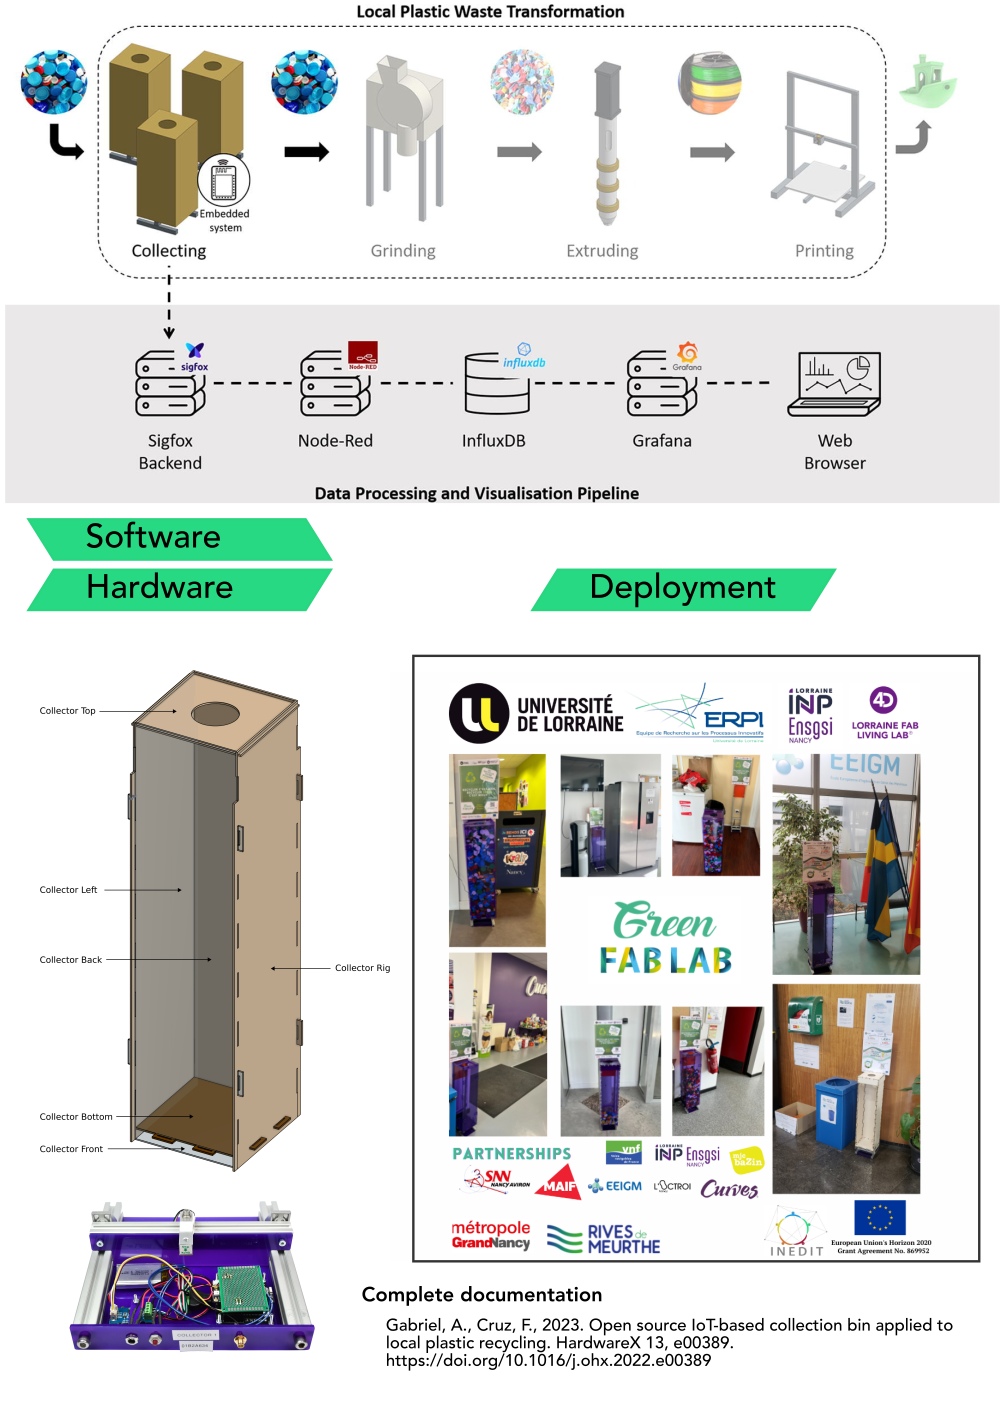
\includegraphics[width=4.16667in,height=\textheight]{figures/SC/Abstract.png}

}

\caption{\label{fig-smart-collector}Description of the developed Smart
collector}

\end{figure}

This is a relevant strategy given the cross-line of Industry 4.0 and
circular economy, which is opening up fields such as smart waste
management systems options to improve the effectiveness of different
materials, including plastic waste
(\protect\hyperlink{ref-Ranjbari2021}{Ranjbari et al., 2021}) using
information technology tools with the advent of the Internet of Things
(IoT) (\protect\hyperlink{ref-fatimah2020}{Fatimah et al., 2020};
\protect\hyperlink{ref-rejeb2022}{Rejeb et al., 2022}). Smart waste
management system (SWMS) consists of public garbage collectors with
embedded technology that is used to monitor real-time level of garbage
bins in public places (\protect\hyperlink{ref-Bano2020}{Bano et al.,
2020}). The interest of this system is to optimize the path for the
garbage collecting van that eventually reduces fuel cost. However, this
work is mainly based on simulation. Therefore, there is an avenue to
simplify experimentation in this domain using common open-source
technology (hardware and software)
(\protect\hyperlink{ref-Pearce2009}{Pearce and Mushtaq, 2009}) to
implement projects that require heavy infrastructure such as routers and
a gateway to deploy in the territory.

The main functional requirement of the smart collector is to collect and
provide data about plastic waste production in order to design a local
and distributed recycling chain of value. However, the smart collector
may be used in various use cases such as:

\begin{itemize}
\tightlist
\item
  Monitoring the quantity of any other product that is collected over a
  large area.\\
\item
  Generating data about behavior to more precisely dimensions public
  infrastructure.\\
\item
  Monitoring the transformation and recycling process inside the
  transformation unit to follow the state and quantity of raw material
  and final product.\\
\item
  Initiating a digitization process in the waste management process as
  the information system element present here is flexible and commonly
  used in various types of projects.
\end{itemize}

The device uses a controller compatible with batteries and uses WAN
technology to avoid the deployment of routers for data acquisition.
Although using various types of sensors allows us to achieve better
results (\protect\hyperlink{ref-Catania2014}{Catania and Ventura, 2014})
by crossing data, the main indicator remains the weight.

The process illustrated by the Figure~\ref{fig-smart-collector} can be
described in the as follows:

\begin{enumerate}
\def\labelenumi{\arabic{enumi}.}
\item
  \textbf{Smart Collector installation}: The first step is to identify
  the main actors in the neighborhood through meetings, visits and
  interviews in order to propose integration into the recycling network
  by installing a smart collector on their premises.
\item
  \textbf{Supervision}: The monitoring is done through a dashboard that
  provides direct information sent by the smart collector. This allows
  to know the weight of each installed smart collector, allowing to have
  an approximation of its degree of occupancy.
\item
  \textbf{Receiving and storing plastic waste}: The storage area must be
  organized and functional with respect to the needs of the
  demonstrator.
\item
  \textbf{Plan and execute the collection}: This step aims to establish
  the collection routine.
\end{enumerate}

The main result is to guarantee a constant supply chain of raw material
that can be used inside the recycling facilities

\hypertarget{preparation-ii}{%
\subsubsection{Preparation II}\label{preparation-ii}}

The second phase corresponds to the actions and processes to identify,
separate, sort, size reduction and clean plastic waste. The main purpose
is to guarantee an adequate feedstock material for the distributed
recycling process. Figure~\ref{fig-adequation} displays an overview of
the space and the machines used in the Green Fablab facilities to treat
the plastic waste.

\begin{figure}[H]

{\centering 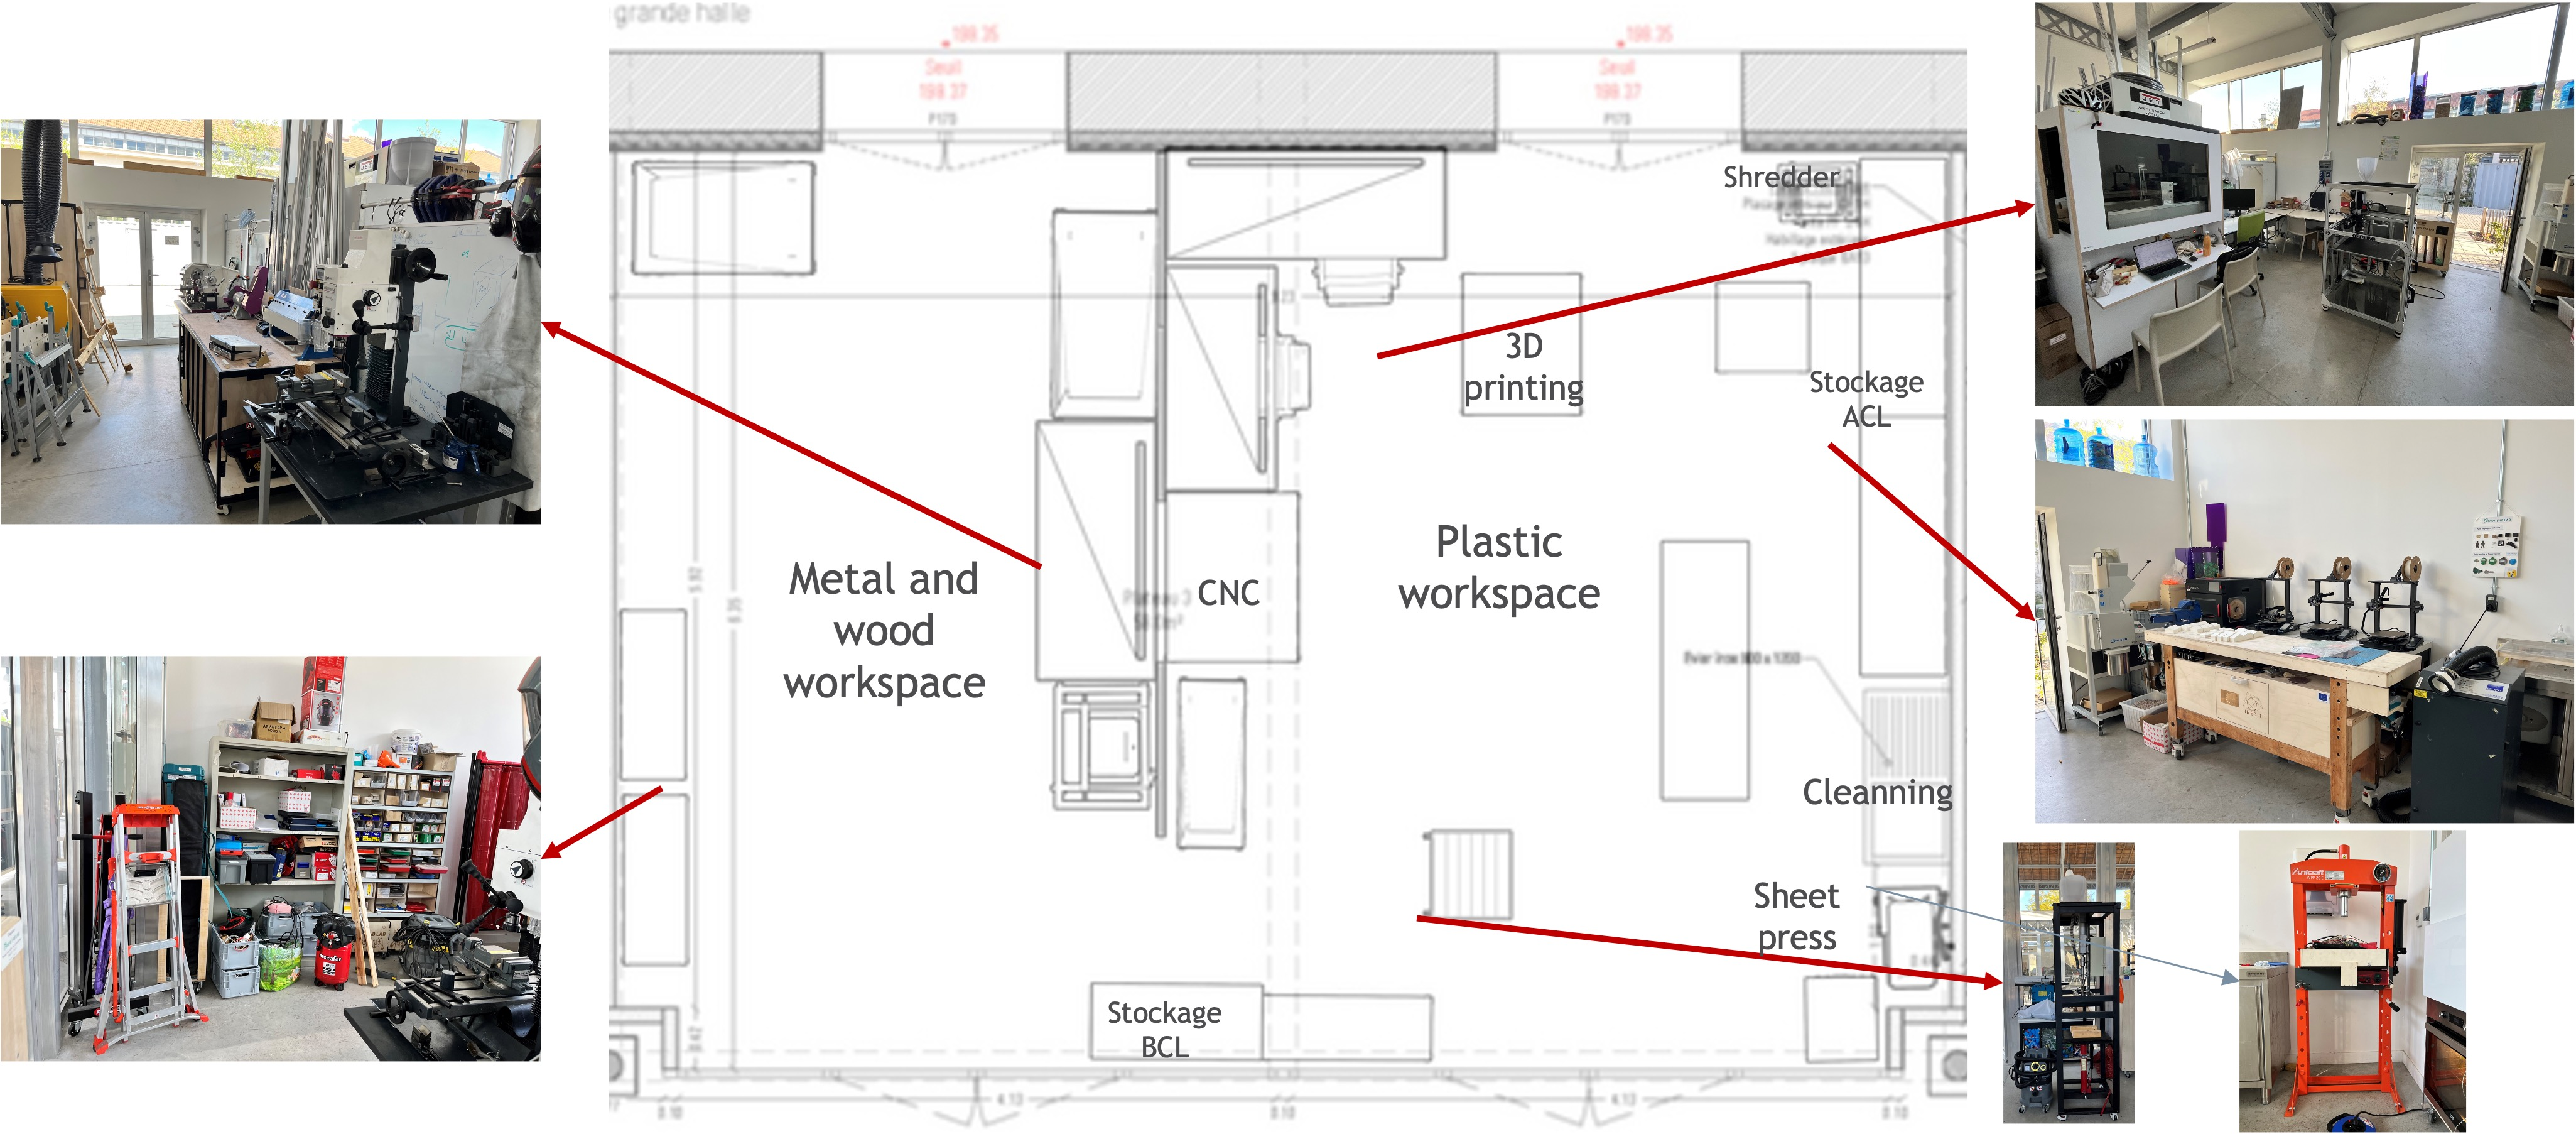
\includegraphics{figures/preparation/adequation.jpg}

}

\caption{\label{fig-adequation}Adequation spaces for the preparation of
the waste material}

\end{figure}

The plastic waste preparation process aims to adequate the collected
plastic to the requirements of 3D printing and manual injection molding.
Four main sub-processes are considered:

\begin{itemize}
\item
  \textbf{Identification and Sorting}: These two processes aim to
  identify the type of plastic given the regular standard for the
  polymer industry. The process of identification and separation of
  plastics is done manually and allows us to separate the plastics that
  can be used as raw material for further production processes.
\item
  \textbf{Cleaning}: This process aims to remove the traces of any other
  substance that may be present in the plastic waste. In this way the
  processing machines will not be exposed to possible anomalies linked
  to material impurities.
\item
  \textbf{Size reduction}: The size reduction process is carried out to
  obtain an adequate granulometry. This process allows the plastic waste
  for the direct injection process and/or the extrusion process.
\item
  \textbf{Drying phase}: This step prevents the formation of bubbles in
  the recycled material when it is melted during the following extrusion
  step. Moreover, complete elimination of water prevents hydrolytic
  decomposition of the molecular chains during the melting or
  plasticization, so that the treated material has to be as dry as
  possible.
\end{itemize}

\hypertarget{compounding-iii}{%
\subsubsection{Compounding III}\label{compounding-iii}}

The \emph{Compounding} III phase is related to the operation, strategies
in the development of composite materials using recycled feedstock
intended for the printing process. There have been several literature
reviews about the technical aspect of composite materials in the
additive manufacturing context
(\protect\hyperlink{ref-Brenken2017}{Brenken et al., 2018};
\protect\hyperlink{ref-Hofstatter2017}{Hofstätter et al., 2017};
\protect\hyperlink{ref-Mohan2017}{Mohan et al., 2017};
\protect\hyperlink{ref-Singh2017}{Singh et al., 2017}).

In the context of the Green Fablab demonstrator of INEDIT project, the
focus is to study the 1) mono-recycled material and 2) the
virgin-recycled blend material. The development of recycling niches of
mono-material where the additive manufacturing can be implemented is key
to study. However, it has to be highlighted that one major assumption of
the scientific studies relies in that the material used is already
sorted, cleaned and using the same type of discarded product.

In INEDIT, the interest is to take into account the inner variability
that could be in the recovery process, concerning the type of material
given the fact, while there are seven types of recycling symbols for
each type of polymer, one major constraint in the current systems is
that each manufacturing company have a patented use of the additive in
the polymer matrix, in order to fulfill its initial function of the
product.

\hypertarget{feedstock-iv}{%
\subsubsection{Feedstock IV}\label{feedstock-iv}}

The \emph{Feedstock} IV phase refers to the processes in order to
transform the plastic waste into usable material for the fabrication
stage. Two outputs are seen here: 1) the filament feedstock and 2) the
pellet feedstock. The use of filament or pellet material are in
coherence with the machine process used in the fabrication.

The filament and pellet production process makes it possible to produce
the necessary raw material from plastic waste. The production of these
intermediate products allows the use of different technologies related.
Before using these products (filaments and pellets) it is necessary to
carry out evaluation tests to assess the geometrical characteristics
that are necessary in the printing process.

The filament production is made using a semi-open source commercial
desktop extruder. Figure~\ref{fig-feedstock} present the technical
characteristics of the material equipment:

\begin{figure}[H]

{\centering 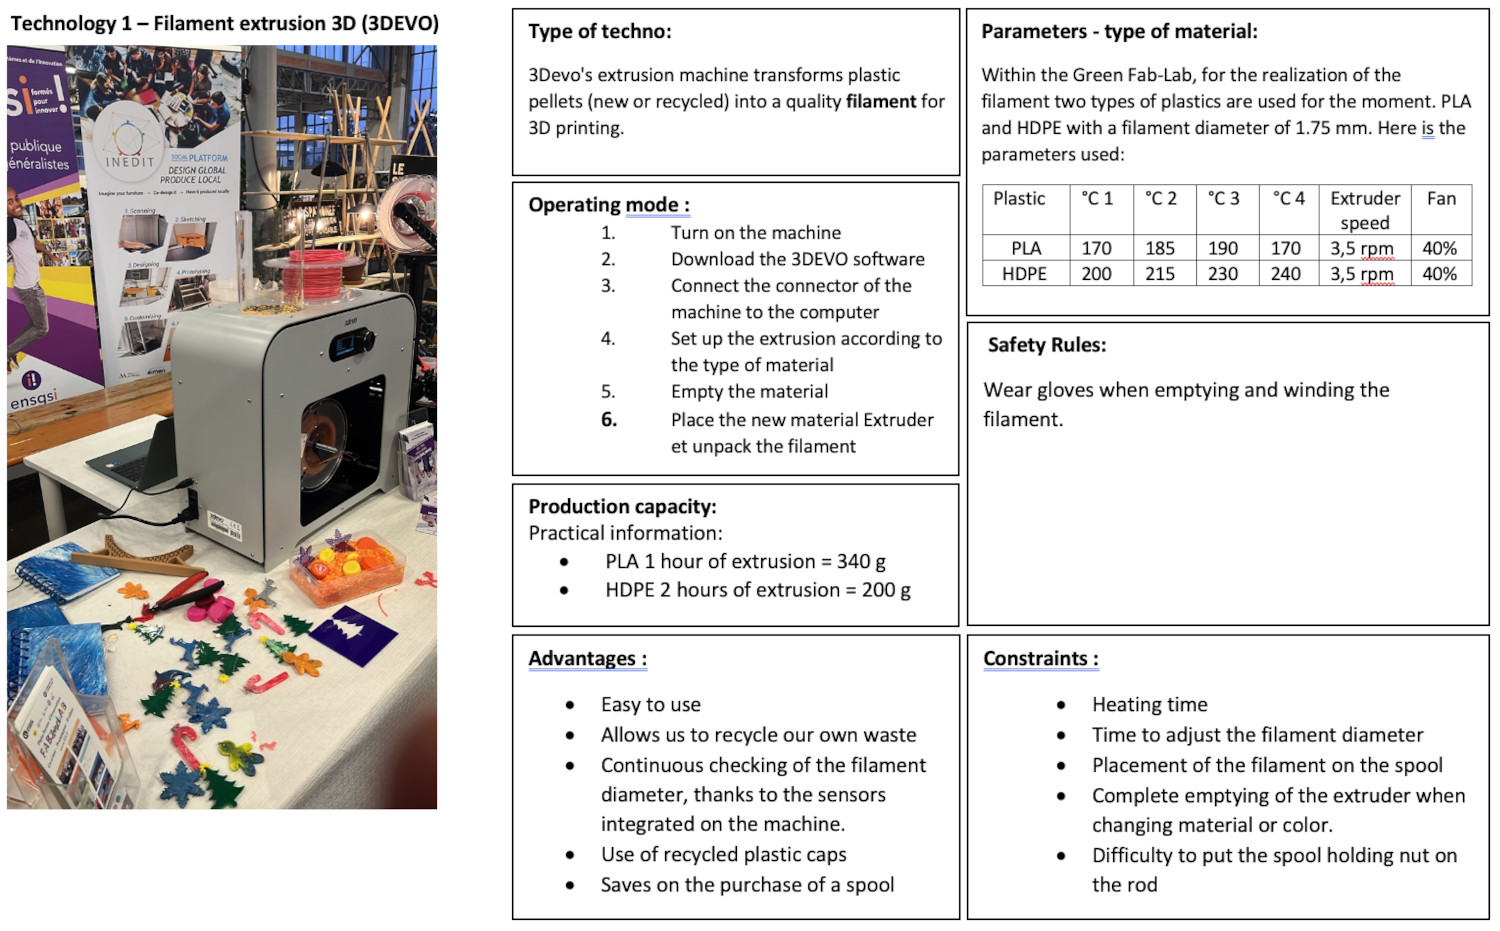
\includegraphics[width=0.9\textwidth,height=\textheight]{figures/feedstock/3devo-00.jpg}

}

\caption{\label{fig-feedstock}Extrusion machine to fabricate recycled
filament feedstock}

\end{figure}

Filament is produced at 0.4 kg/h using 0.24 kWh/kg with a diameter
±4.6\%.

\hypertarget{printing-process-v-and-desktop-injection-molding}{%
\subsubsection{Printing process V (and desktop injection
molding)}\label{printing-process-v-and-desktop-injection-molding}}

In this step, the major output is the valorisation of the plastic waste
material using different two alternative paths: 1) desktop injection
molding process (small and medium sizes), and 2), 3D printing process
(fused filament fabrication --FFF- and fused granular fabrication
--FGF-).

As matter of the validation of the demonstrator at TRL 6 level, the
ambition of the demonstrator in the INEDIT project is to experiment and
prove a technological ecosystem mix that seeks to valorise in a
distributed approach different plastics for different purposes and
stakeholders. Therefore, the initial choice is these two paths to create
objects injected and 3D printed parts that are useful to the local
ecosystem of the demonstrator. The technologies are presented in the
following paragraphs.

\hypertarget{desktop-injection-molding}{%
\paragraph{Desktop injection molding}\label{desktop-injection-molding}}

Injection molding is one of the most used techniques to form plastic
materials.\\
Figure~\ref{fig-injection} presents the major technologies in the `Green
Fablab' case to propose a manual recycled aspect to reuse the plastic
waste into small and medium plastics sheets.

\begin{figure}[H]

{\centering 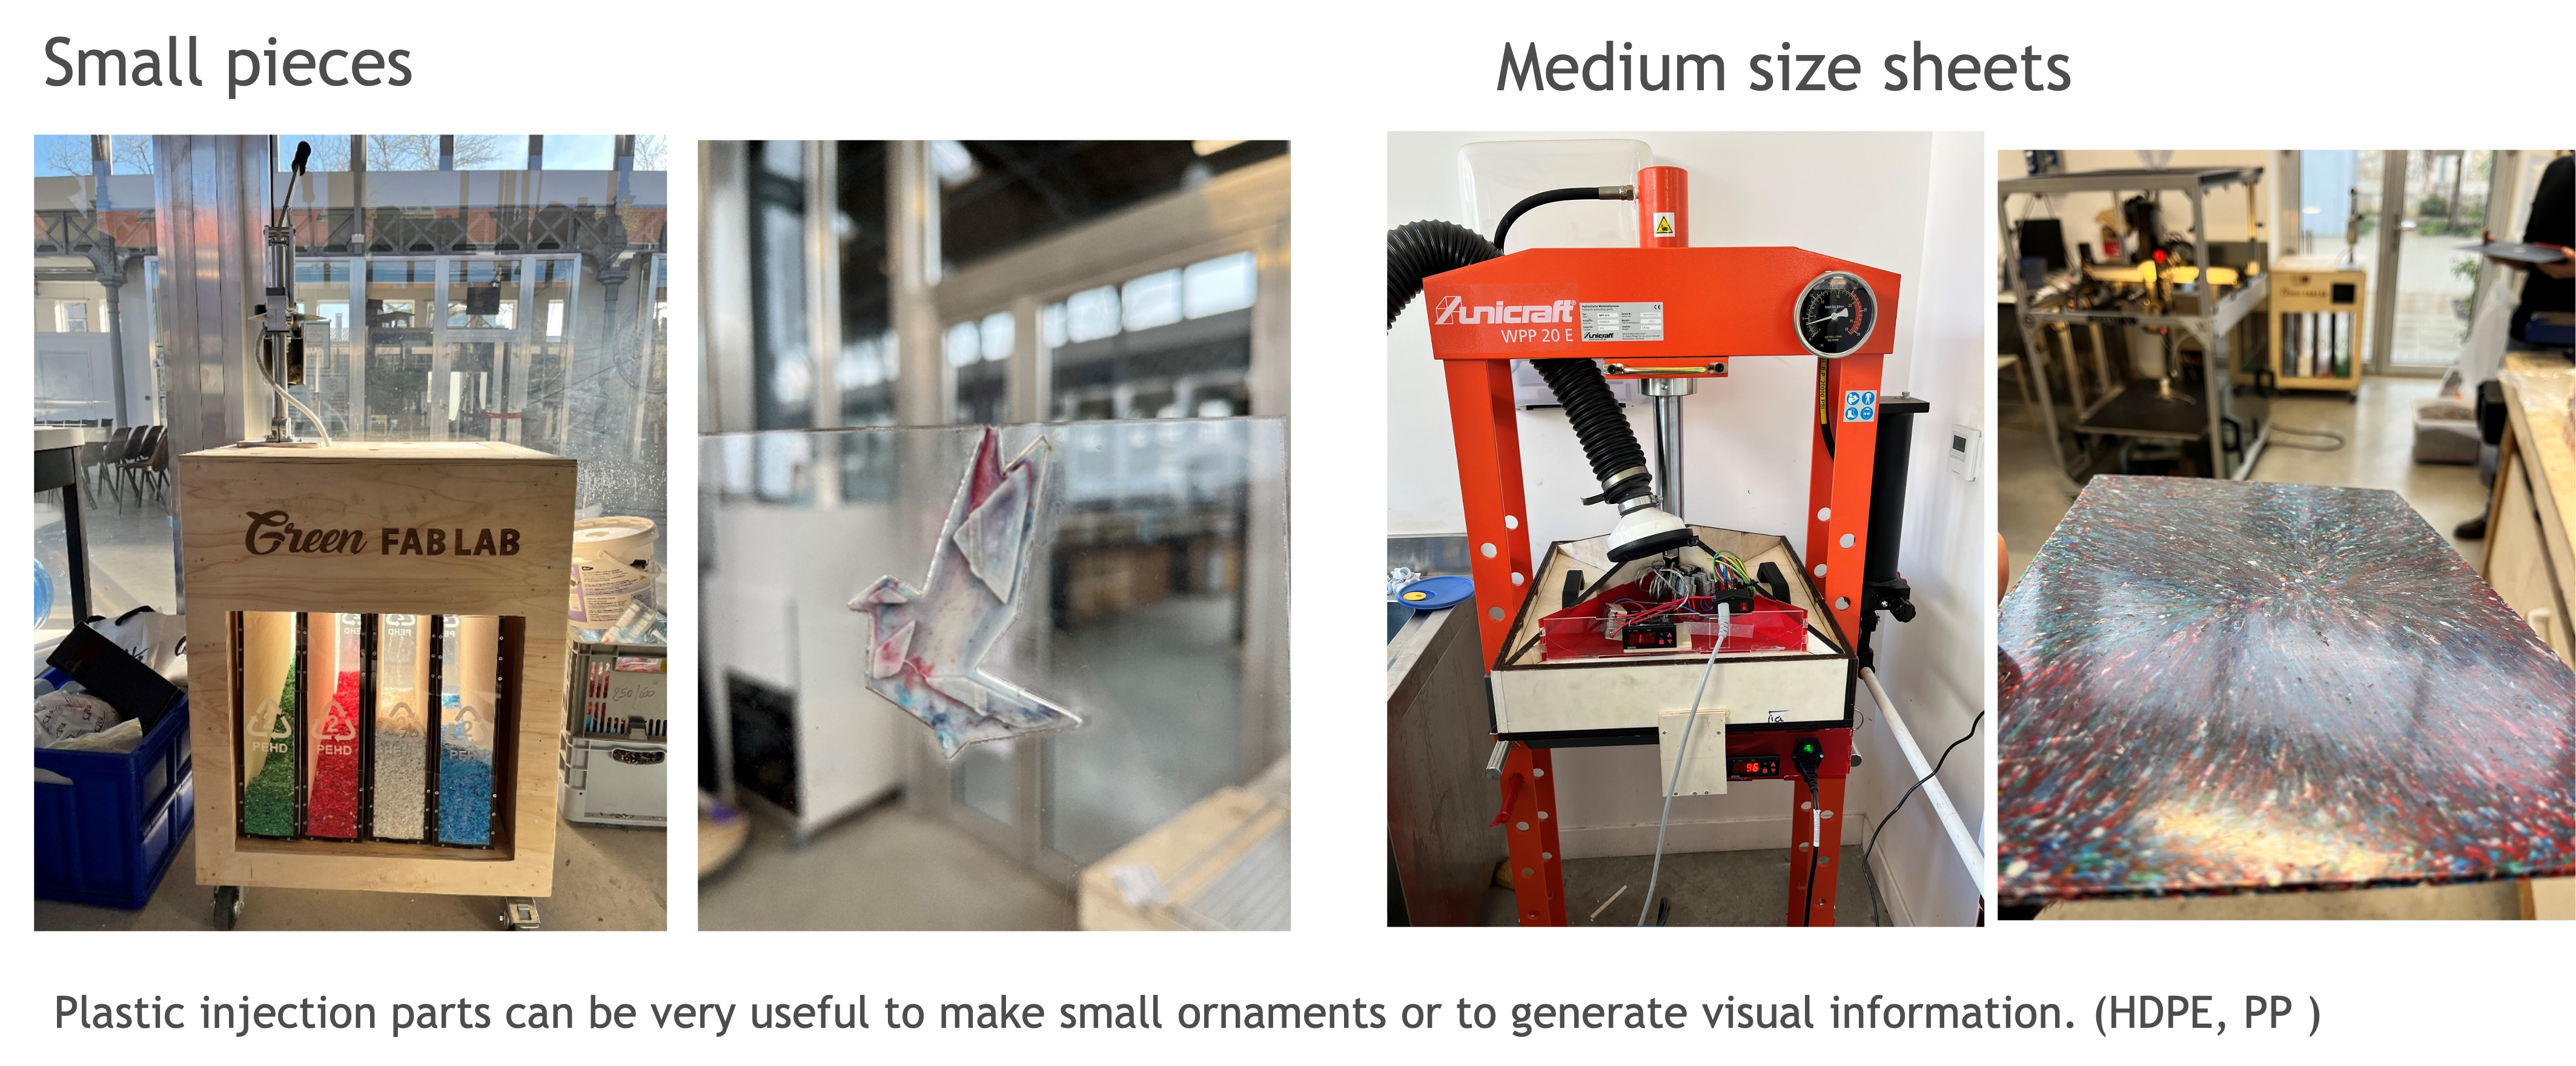
\includegraphics[width=0.9\textwidth,height=\textheight]{figures/printing/injectin-00.jpg}

}

\caption{\label{fig-injection}Manual injection in small and medium
sizes}

\end{figure}

\hypertarget{d-printing-process-fused-filament-granular-fabrication-fff-fgf}{%
\paragraph{3D printing process: Fused Filament \& Granular Fabrication
(FFF \&
FGF)}\label{d-printing-process-fused-filament-granular-fabrication-fff-fgf}}

In the era of additive manufacturing technology, without a doubt, the
material extrusion-based systems such as the fused filament fabrication
(FFF) has been one of the prominent processes. In fact, the
technological development of open-source 3D printers is creating more
affordable Additive Manufacturing (AM) machines for society in different
applications. It provides the possibility of mass diffusion of this
technology, and consequently, AM is being recognised as a disruptive
that could up-end the last two centuries of approaches to design and
manufacturing (\protect\hyperlink{ref-Birtchnell2013a}{Birtchnell and
Urry, 2013}).

In the Green Fablab demonstrator, we have two types of material-based
systems: 1) Fused filament fabrication (FFF) and 2) Fused Granular
Fabrication (FGF):

\begin{figure}

\begin{minipage}[t]{0.67\linewidth}

{\centering 

\raisebox{-\height}{

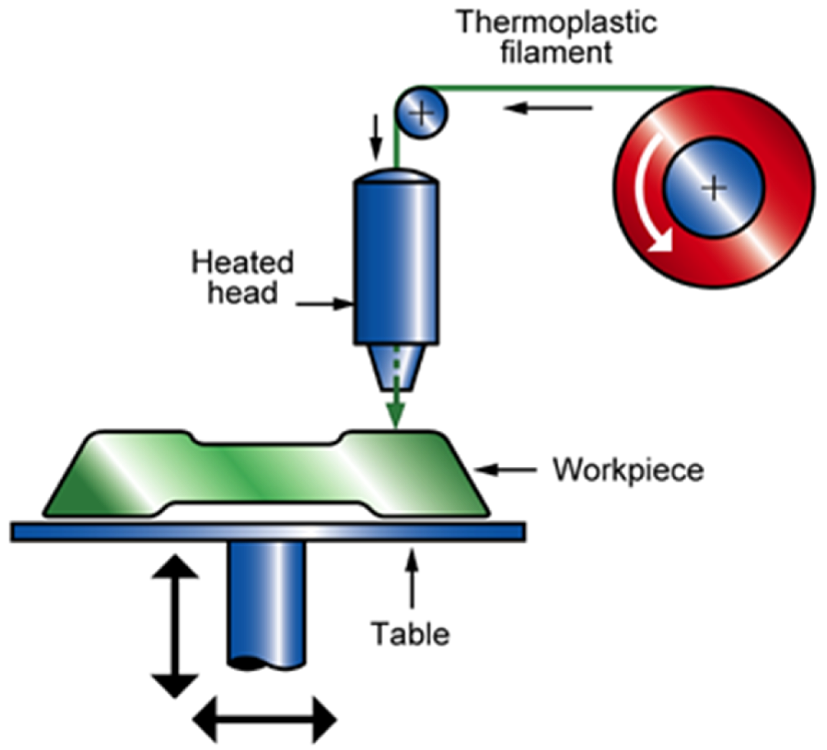
\includegraphics[width=2.08333in,height=\textheight]{figures/FFF-00.png}

}

}

\subcaption{\label{fig-fff}Fused filament fabrication -FFF- principle}
\end{minipage}%
%
\begin{minipage}[t]{0.33\linewidth}

{\centering 

\raisebox{-\height}{

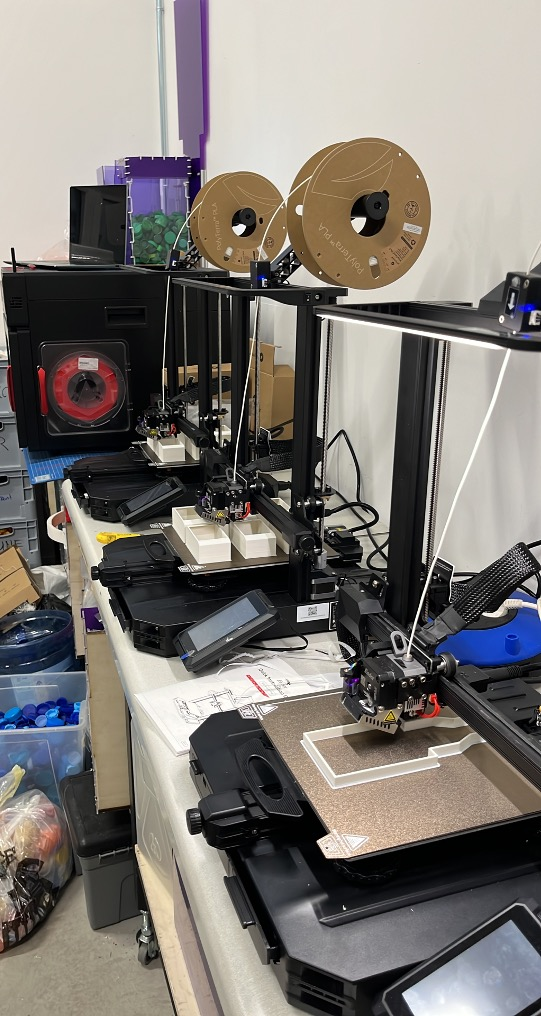
\includegraphics[width=1.04167in,height=\textheight]{figures/printing/FFF.jpg}

}

}

\subcaption{\label{fig-fff}3D printinter machines}
\end{minipage}%

\caption{\label{fig-fff}Fused filament fabrication machines}

\end{figure}

The principle of the filament fabrication was developed and patented in
1989 by Scott Crump as \emph{Fused Deposition Modeling}, and since 2009,
the technology became open source, known as Fused Filament Fabrication,
to establish the difference between the registered mark. A schematic
representation of this technology is presented in Figure~\ref{fig-fff}.
This process usually uses thermoplastic polymer filaments that are
heated until a temperature slightly higher than the melting temperature
at the nozzle of the machine, reaching a semi-liquid state. At this
point, the polymer is extruded on the platform to create the first layer
of the object and after that, the polymer continues to be printed on top
of the previous layer, so that, filament fuses with the previous layer
and then is solidified at room temperature after printing
(\protect\hyperlink{ref-CruzSanchez2017}{Cruz Sanchez et al., 2017};
\protect\hyperlink{ref-Ngo2018}{Ngo et al., 2018}).

On the other hand, Fused granular fabrication --FGF- is a polymeric
additive manufacturing process which make use of pellets rather than
traditional filaments as feedstock material The FGF is a new key
additive manufacturing process and it is a key technical advancement to
facilitate the use of recycled material in the printing process.
Figure~\ref{fig-gigabot} presents the Gigabot X XL machine used in the
experimentation.

\begin{figure}

\begin{minipage}[t]{0.67\linewidth}

{\centering 

\raisebox{-\height}{

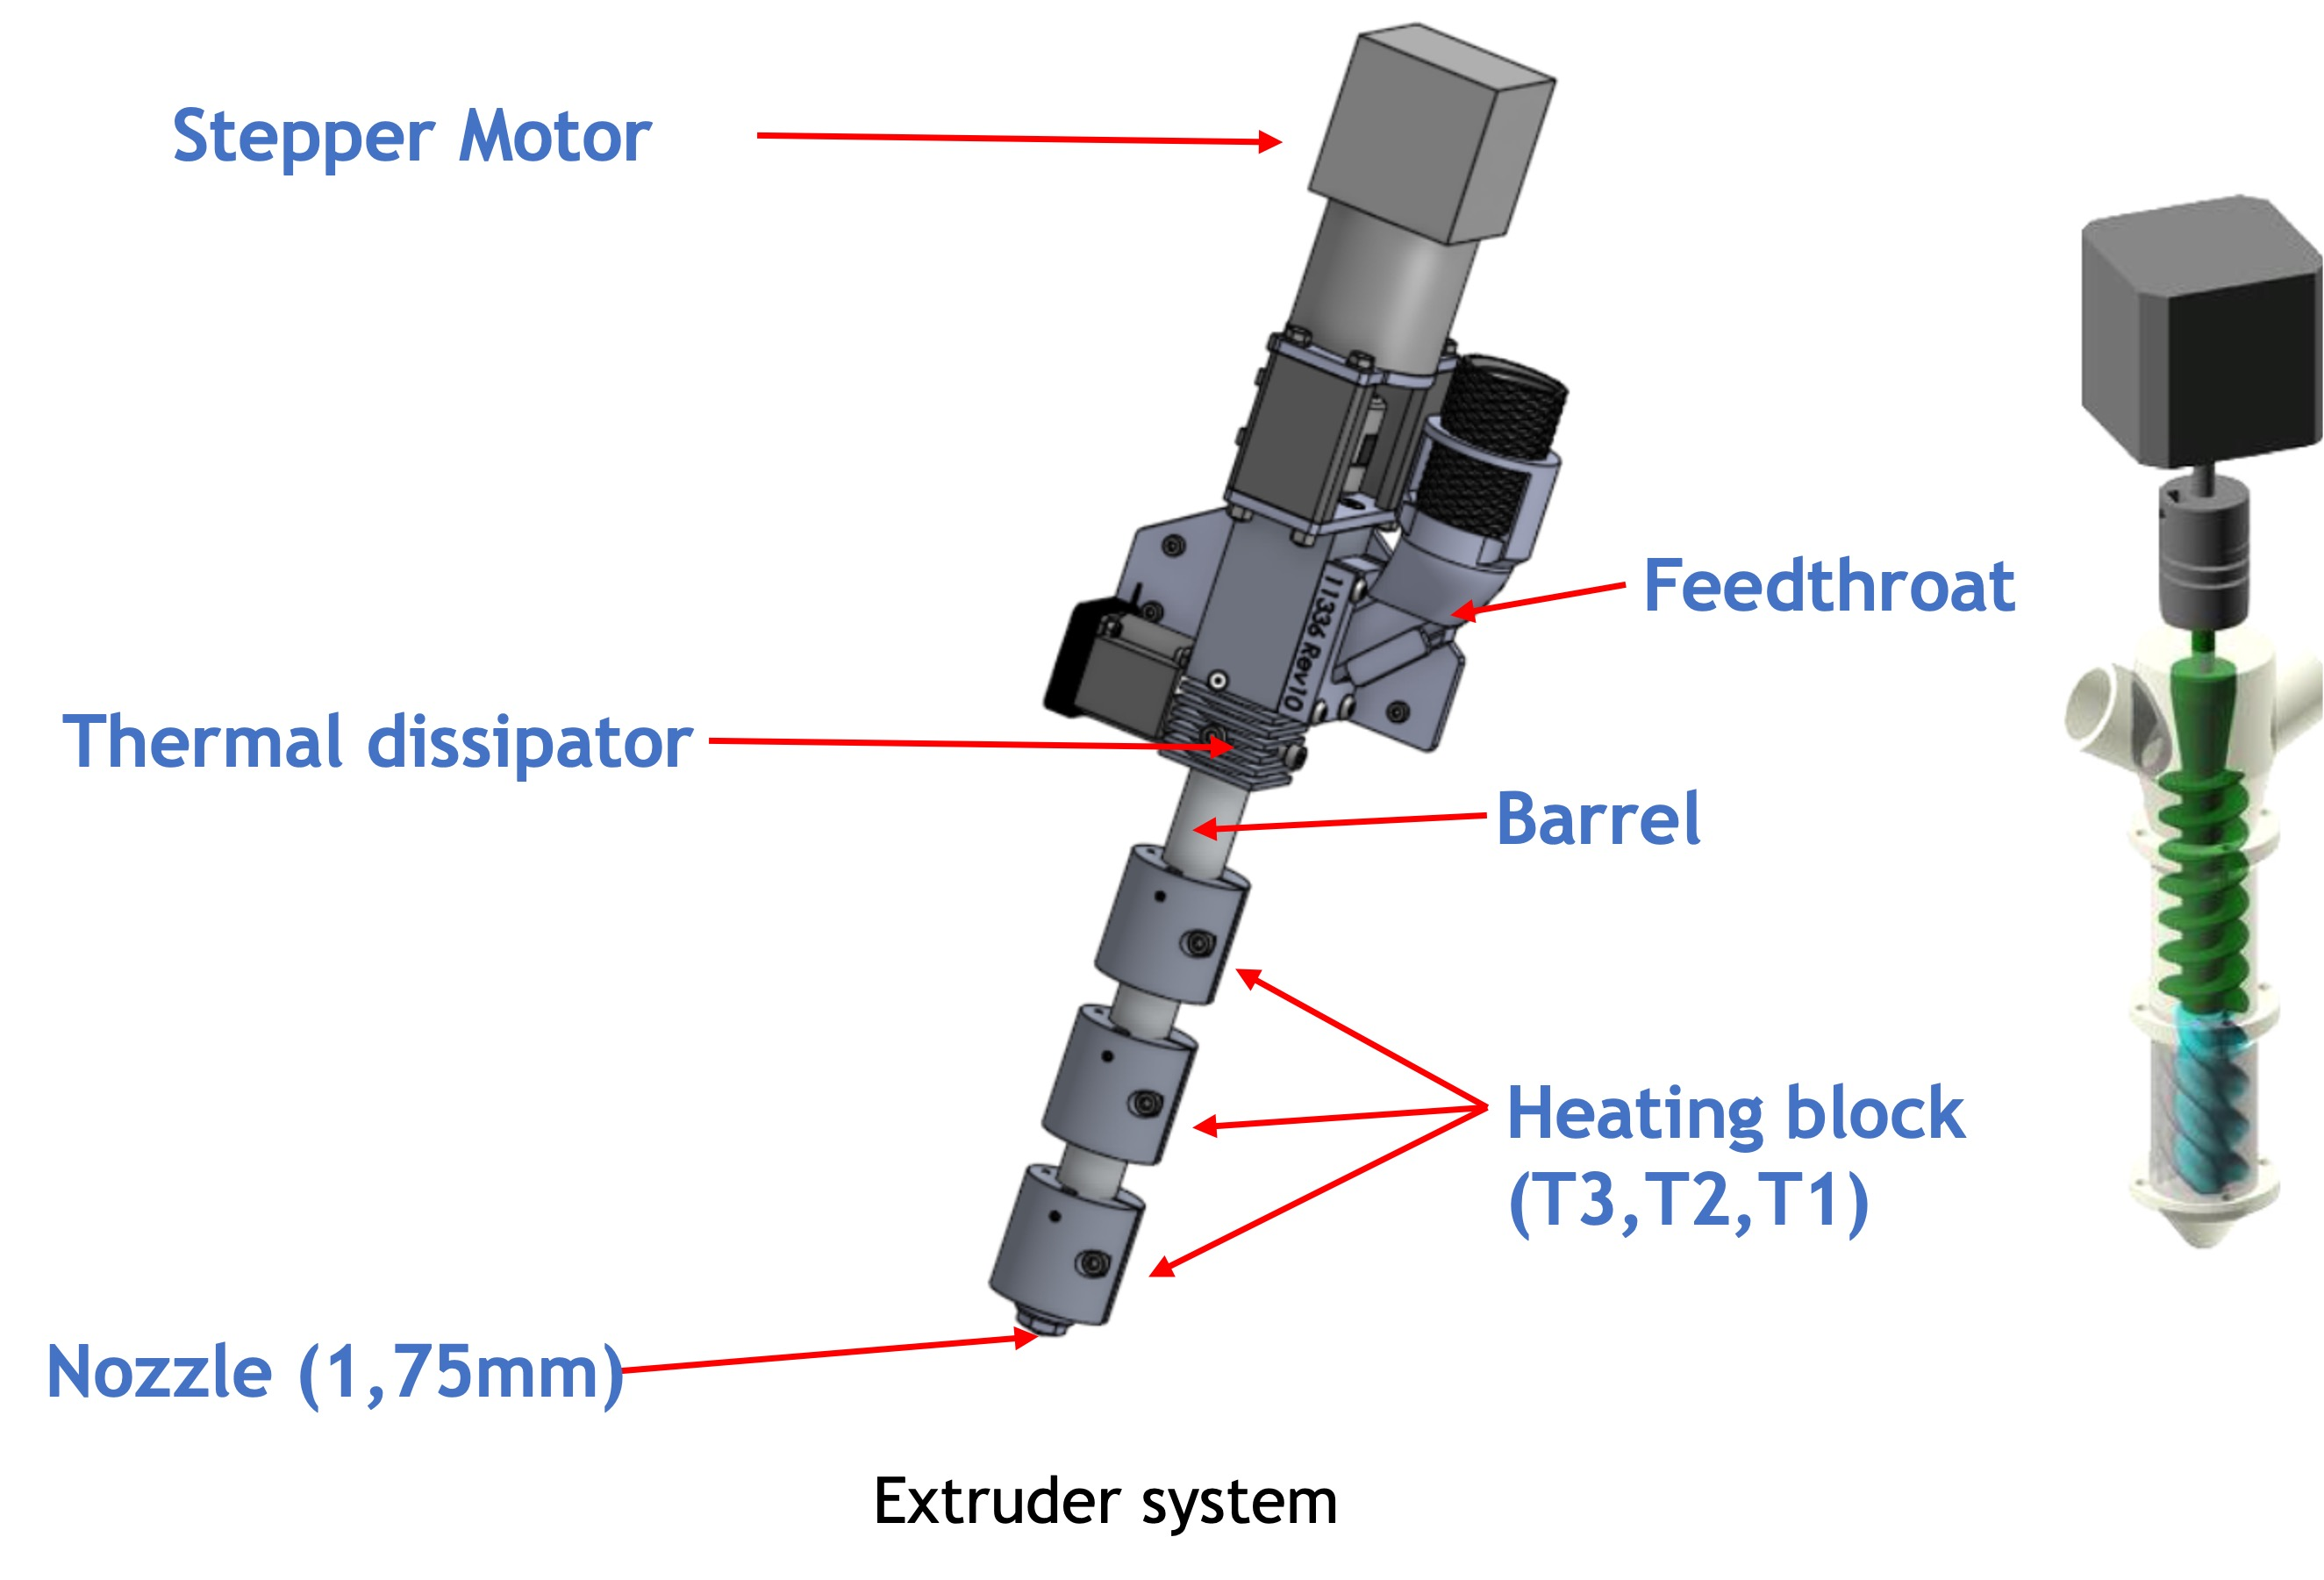
\includegraphics[width=3.125in,height=\textheight]{figures/printing/gigabot-concept.jpg}

}

}

\subcaption{\label{fig-fff}Fused Granular fabrication -FFF- principle}
\end{minipage}%
%
\begin{minipage}[t]{0.33\linewidth}

{\centering 

\raisebox{-\height}{

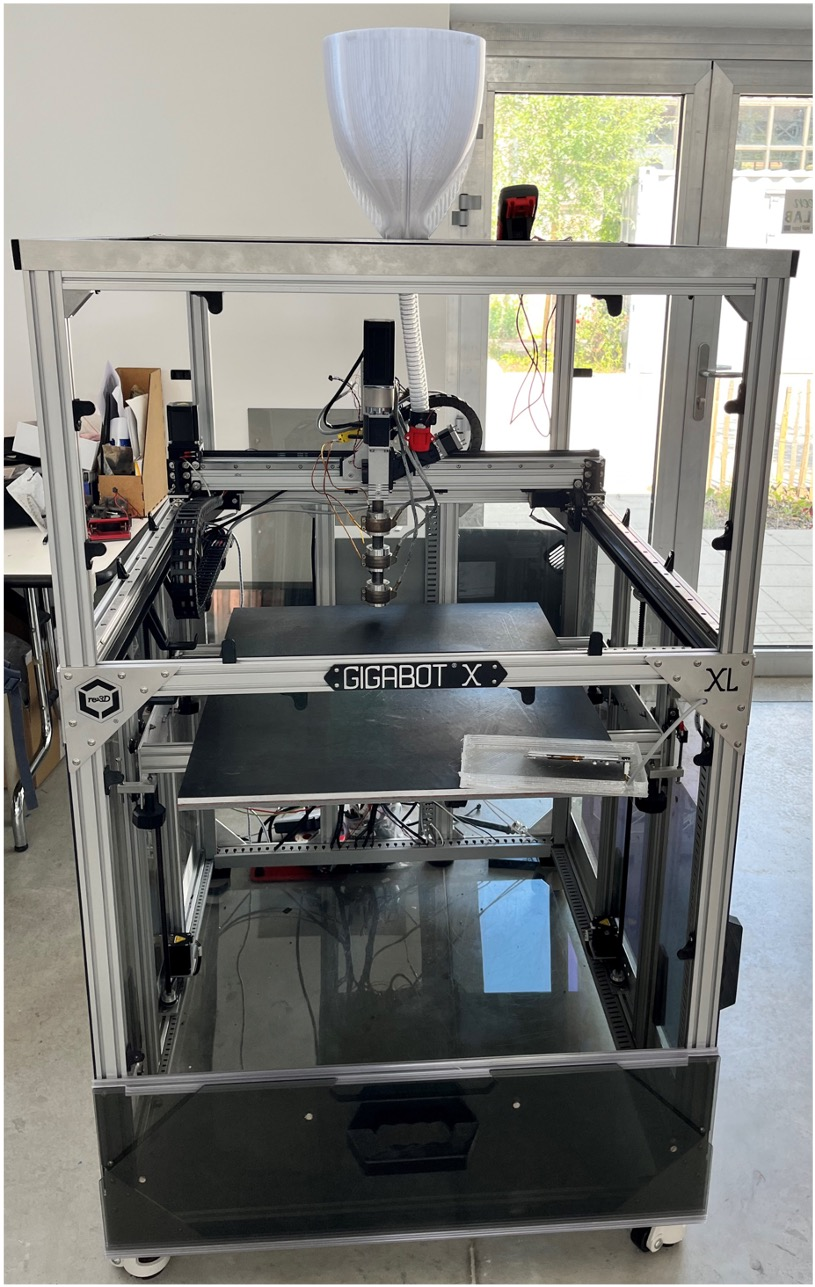
\includegraphics[width=1.5625in,height=\textheight]{figures/printing/Gigabot-2.jpg}

}

}

\subcaption{\label{fig-fff}Gigaboot X XL printer}
\end{minipage}%

\caption{\label{fig-gigabot}Fused Granular Fabrication fabrication}

\end{figure}

Heating blocks provide sufficient heat energy to change the pellets from
solid stated to liquid state and the compression screw helps in
providing enough pressure to push the liquefied thermoplastic. This
machine has a long barrel with 3 heating elements or zones which helps
in the melting of the thermoplastic. There are three main temperatures
T1 being the heating block near the nozzle while T2 being in the middle
of T1 and T3. Gigabot X XL is equipped with a nozzle of 1.75mm diameter
that influences the deposition rate.

The design of compression screw is also important for efficient melting
of the material and to create back pressure to remove the trapped air
inside the barrel. Convectional extruder screw has 3 section -- feeding
section, melting section, and metering section.

The quality of the extruded material or print quality depends on process
parameters of the machine. The print quality is distinguished into two
parts visual inspection and quantitative measurements. Visual inspection
is the direct inspection of the 3D printed part however quantitative
inspection is the measurements of the dimension of the 3D printed part.
The resolution of 3D printer is causally related to the size of the
nozzle. Small sized nozzles produce small details accurately as the
smallest feature size is reduced to the diameter of the nozzle. The
smallest nozzle size diameter ranges from 0.15 -- 0.7 mm. While small
nozzle size provides good print resolution big nozzle diameters increase
mass flowrate which reduce the production time. Large nozzle diameter
ranges (from 5 -- 7.62 mm) provides a decent print resolution and good
mass flowrate. A detailed description is presented in the annex A to
present the technology.

In the following section, we present how was the operationalization of
the DIT for the 3D printing of recycled Plastic demonstrator.

\newpage

\hypertarget{sec-dit}{%
\section{Operationalization of DIT process for the Use
Case}\label{sec-dit}}

\hypertarget{integration-of-the-3d-printing-recycled-plastic}{%
\subsection{Integration of the 3D Printing Recycled
Plastic}\label{integration-of-the-3d-printing-recycled-plastic}}

The following table presents an explanation of the implementation steps
for the use case. In the next subsections each step will be detailed.

\begin{table}[H]
\centering\begingroup\fontsize{10}{12}\selectfont

\begin{tabular}[t]{>{\raggedright\arraybackslash}p{4cm}>{\raggedright\arraybackslash}p{12cm}}
\toprule
Steps ID  & Steps Description \\
\midrule
\cellcolor{gray!6}{STEP 1 - RECEIVE DESIGN AND SPECIFICATION } & \cellcolor{gray!6}{Information about materials, finish, colour, texture, etc. from the INEDIT platform are sent to the manufacturing centre chosen by the ERP module and the Sustainability Driven Orchestrator (SDO). The expected files to be imported are: CAD file of the object, colour and texture, technical requirements identified in the design phase. }\\
STEP 2 - VALIDATION OF THE TECHNICAL SPECIFICATIONS OF MODEL TO FABRICATE  & Furniture producers or FabLab with the support of 3D printing technical experts evaluate the printability (if the part can be printed with the available technology) as well as validate the design. \\
\cellcolor{gray!6}{STEP 3 - IDENTIFY LOCAL SOURCES OF PLASTIC WASTE } & \cellcolor{gray!6}{This step starts identifying local sources of plastic waste at least 2 km far from the production site. Designers and technicians will evaluate the quantity and quality of possible plastic wastes that could be used as secondary raw material. }\\
STEP 4 – PUT IN PLACE SMART COLLECTOR  & By using the Smart Collector developed by UL in the local areas (< 2 km) it is enabled to collect plastic waste from the sources identified before. \\
\cellcolor{gray!6}{STEP 5 - TRANSPORT WASTE MATERIAL TO THE RECYCLING FACILITIES } & \cellcolor{gray!6}{All the recycled plastic waste is collected and transported to the recycling facilities }\\
\addlinespace
STEP 6 - ADEQUATION AND PREPARATION OF THE MATERIAL, MATERIAL PRINTABILITY VERIFICATION  & The collected material has to be adequate in order to be utilised as recycled feedstock (sorting of usable material, cleaning, etc). The treated material needs to be tested and validated (evaluation on usage and printability). \\
\cellcolor{gray!6}{STEP 7 - PATH PLANNING–3D PRINTING } & \cellcolor{gray!6}{Path planning software generates the best printing strategy to reduce the material used and time. The high-tech solution developed by UL manufactures using at least 30\% of recycled plastic the product in the previously chosen manufacturing centre. }\\
STEP 8 – POST PROCESSING  & If needed, a post-processing phase refines the product in terms of aesthetic quality in order to meet customer requirements. Some parts need to be assembled in the manufacturing site before shipping to the customer. \\
STEP 9 – Implementation Examples & The DIT innovation space enables the designer to test the just realized prototype, to ensure proper functioning in real conditions. 
\cellcolor{gray!6}{If the test by use of the prototype fails, the failure is improved and corrected, repeating the process (re-involving the necessary stakeholders and the technologies used). }\\
Validation & The use case ends validating the product printed, first by the manufacturer and the designer, second by a responsible entity for verification of design feasibility that provides safety and environmental certification and lastly by the customer use (feedback). \\
\bottomrule
\end{tabular}
\endgroup{}
\end{table}

\hypertarget{step-1-receive-design-and-specification}{%
\subsection{Step 1 -- Receive Design and
Specification}\label{step-1-receive-design-and-specification}}

The first step in the reception of the design models and specifications
from the INEDIT platform. The starting point of this activity is
downloading the respective documents that contain the 3D model to be
manufactured by the use case as presented in the Figure~\ref{fig-step1}.

\begin{figure}[H]

{\centering 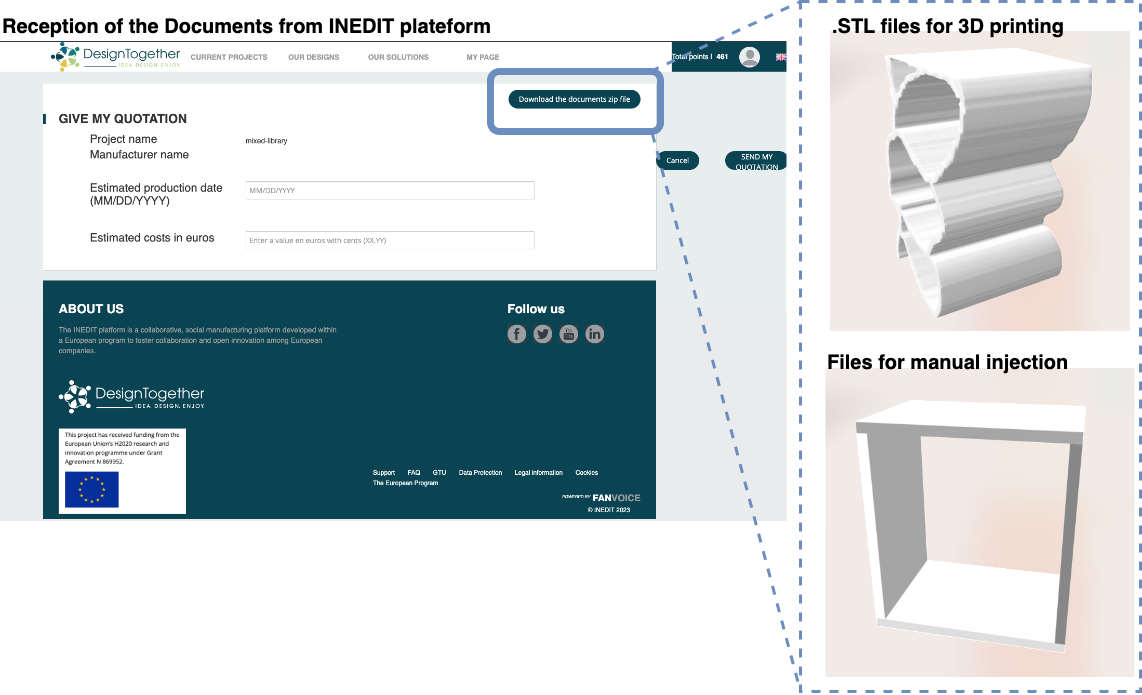
\includegraphics[width=0.8\textwidth,height=\textheight]{figures/Step-1.png}

}

\caption{\label{fig-step1}Reception of the exploitable documents for the
fabrication process}

\end{figure}

One of the outputs of the co-creation phase of INEDIT platform is the
creation of a first initial model that can be exploitable in the open
manufacturing process. In that way, the model is received taking into
account the specific requirements of the customer, and the required
inputs to determine if the technologies available in the demonstration
have the capacity to produce the product. In the case that it cannot be
produced, it is necessary to notify immediately together with the
arguments why it cannot be produced and offer ways of improvement.

\hypertarget{step-2-validation-of-the-technical-specifications-of-model-to-fabricate}{%
\subsection{Step 2 -- Validation of the technical specifications of
model to
fabricate}\label{step-2-validation-of-the-technical-specifications-of-model-to-fabricate}}

The main purpose of the second step is to establish the criteria for the
validation specifications of the model to fabricate. In the case of the
Green FabLab, three main criteria were established concerning:

\begin{figure}[H]

{\centering 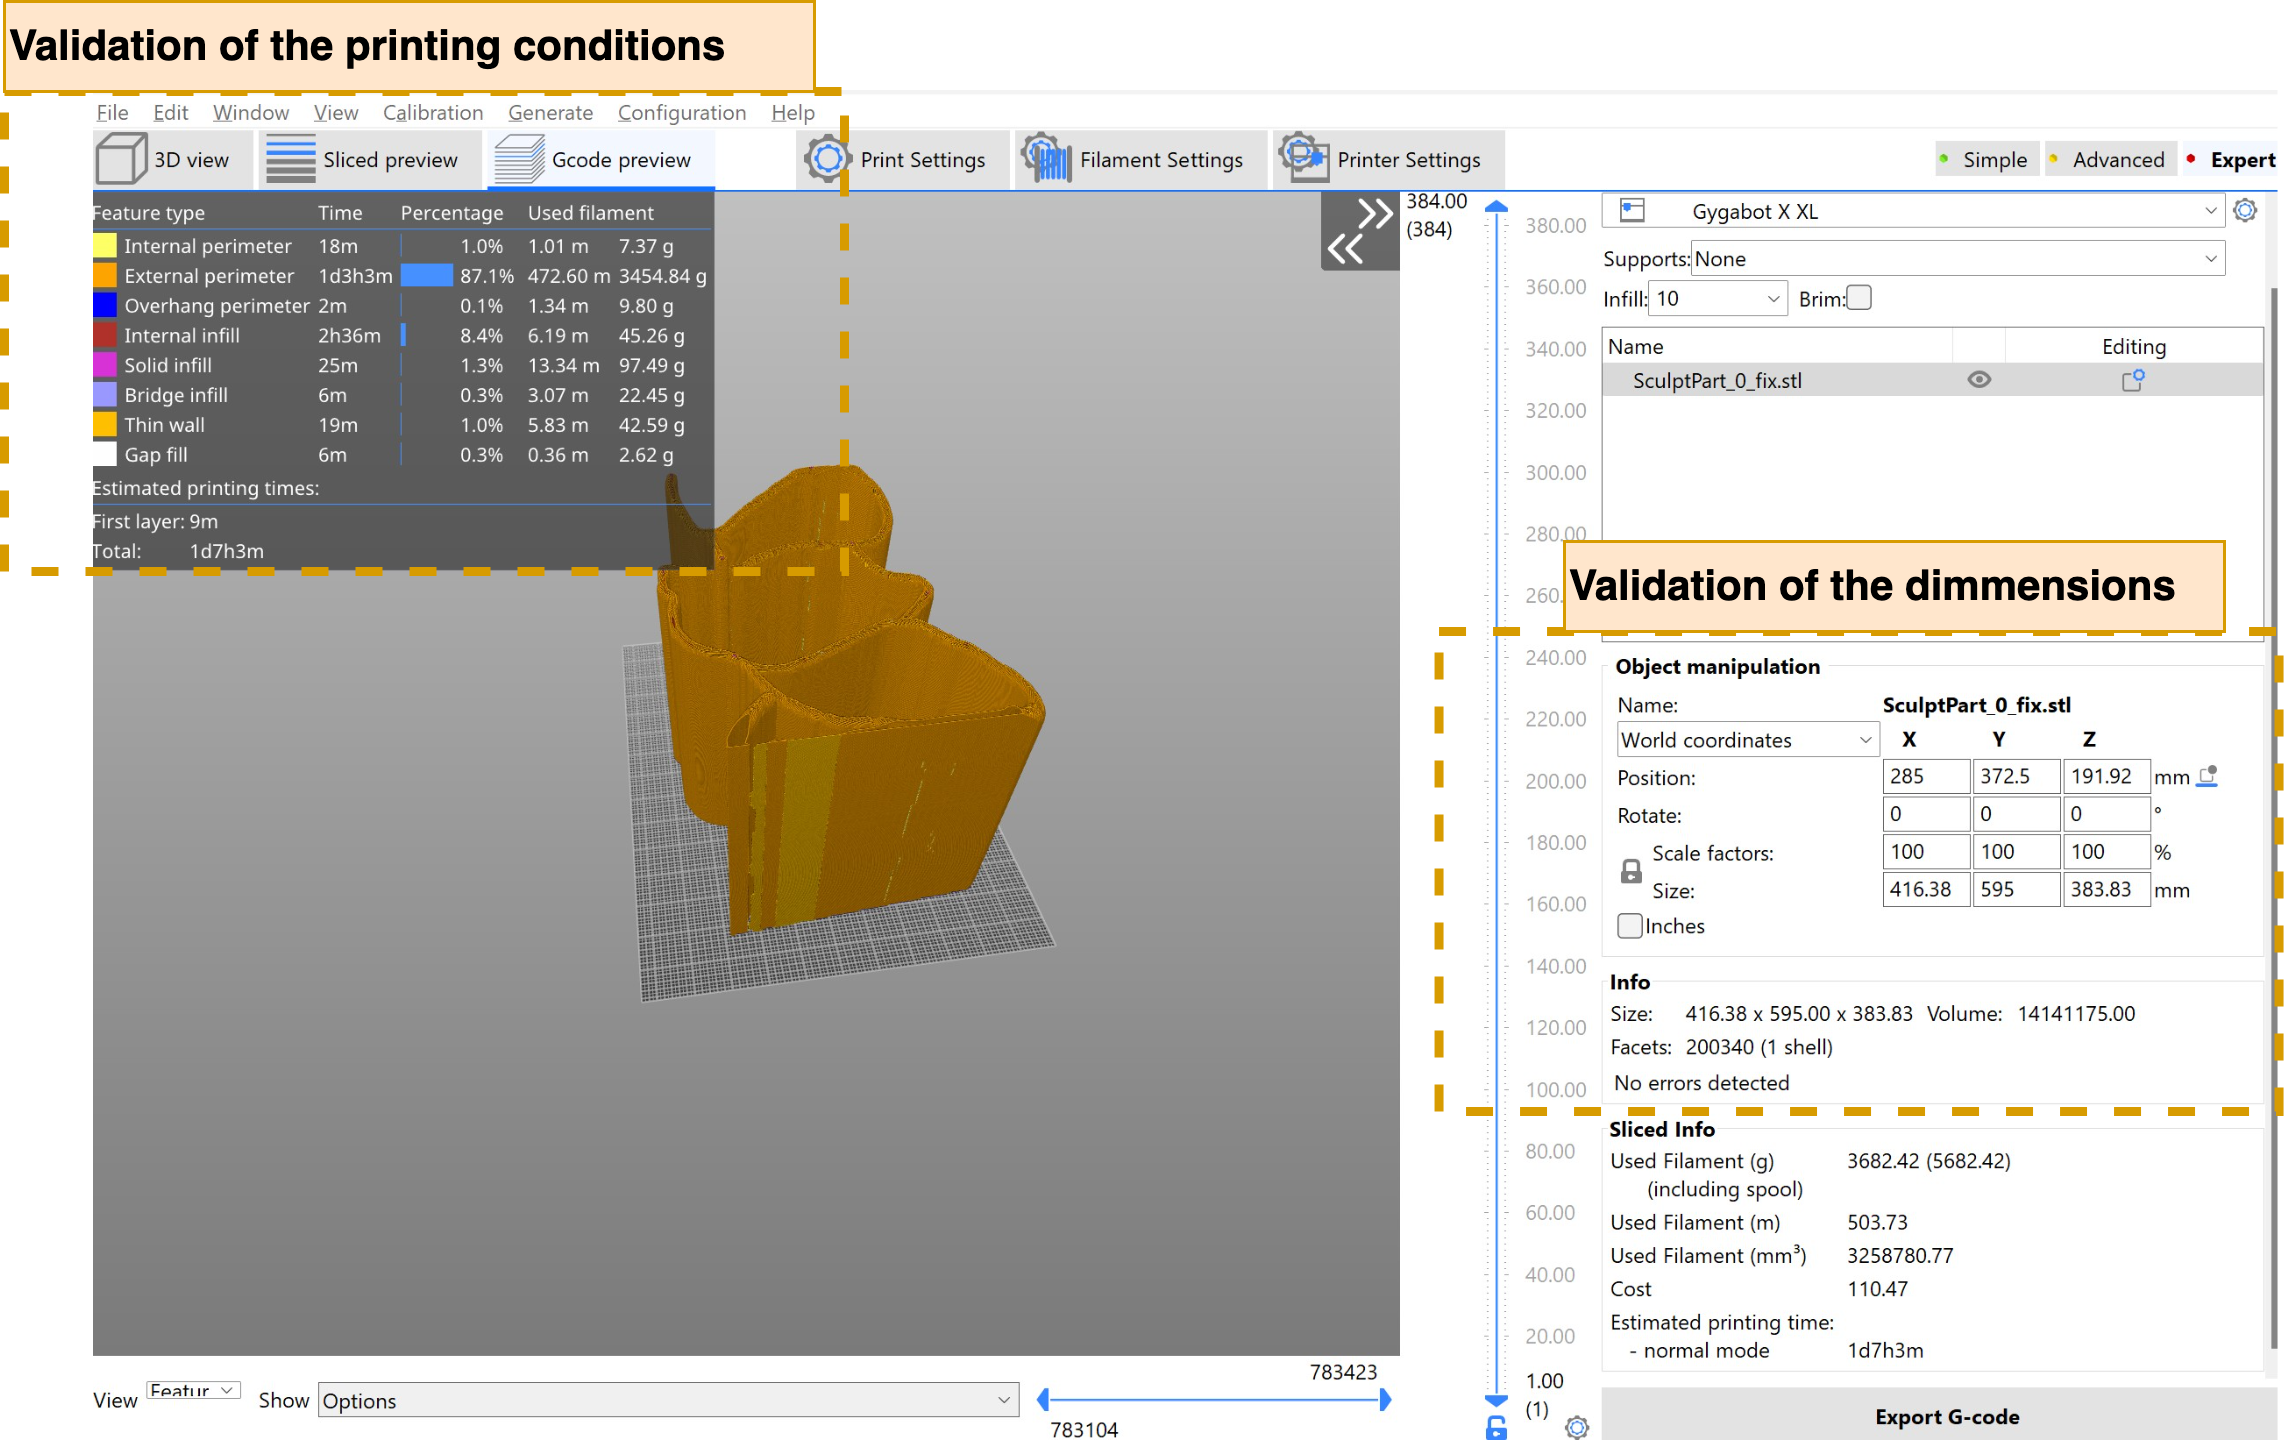
\includegraphics[width=0.9\textwidth,height=\textheight]{figures/Step-2.png}

}

\caption{\label{fig-step2}Validation of the printing conditions}

\end{figure}

\begin{enumerate}
\def\labelenumi{\arabic{enumi}.}
\tightlist
\item
  the dimensions of the part
\item
  the orientation and quality of the STL
\item
  the printability of the material
\end{enumerate}

Using the software SuperSlicer and the machine-specific configuration
(e.g.~for FGF or FFF printer), it is validated that the global
dimensions of the proposed part are coherent. This needs to be in the
range of the maximal working dimensions of the 3D printers.

Lastly, the printability tests are based on the characteristics of the
material and the variables of the machine (namely, the temperatures of
the barrel, the rotation of the stepper motors and the diameter of the
nozzle). Different tests of printability were made in order to have a
baseline of usable printed part as illustrated in the
Figure~\ref{fig-printability}.

\begin{figure}[H]

{\centering 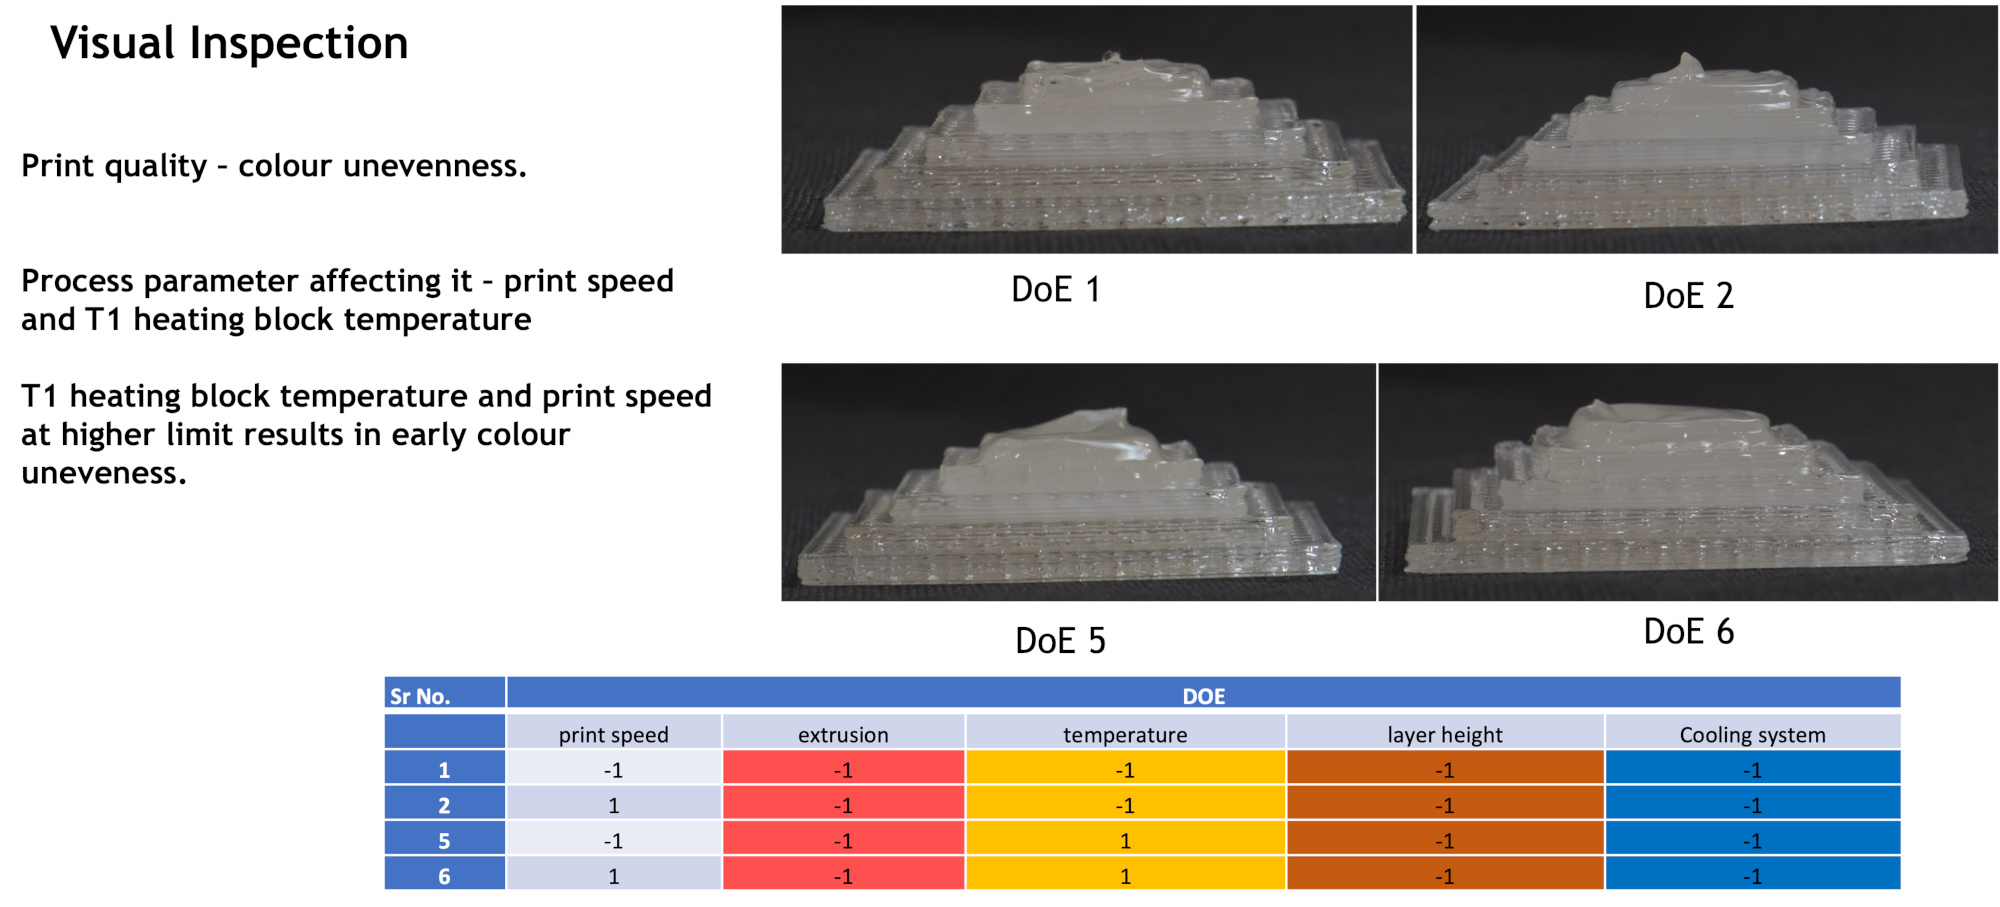
\includegraphics[width=4.6875in,height=\textheight]{figures/Swapnil-Results-02.jpg}

}

\caption{\label{fig-printability}Experimental protocol to validate the
printability tests}

\end{figure}

he test of printability consists in the selection of the technical
parameters of the machine (e.g.~print speed, extrusion factor,
temperature, layer height) using a Design of Experiments (DoE) approach.
Then, with a basic benchmarking model (e.g.~lines, cubes, pyramides), it
is possible to identify the errors in the printing process using
statistical approaches such as ANOVA and measures of standard error.

A technical paper to describe in more detail the results of this
printability approach is being prepared at the time of writing this
final rapport.

\hypertarget{step-3-identify-local-source-of-plastic-waste}{%
\subsection{Step 3 -- Identify local source of plastic
waste}\label{step-3-identify-local-source-of-plastic-waste}}

This step seeks to establish a first network of plastic wastes source
from the local ecosystem. The task of the identification of local
sources of plastic wastes is fundamental as the first stage in the
recovery process. Therefore, an exchange with local key actors was
necessary in order to achieve this task.

The first step was to identify relevant stakeholders in the local
ecosystems to inquire on the issue of plastic wastes sources. Firstly,
they needed to belong to a geographical range perimeter (less than 2km
around the facilities) following the observations of
(\protect\hyperlink{ref-CruzSanchez2020}{Cruz Sanchez et al., 2020};
\protect\hyperlink{ref-Santander2020}{Santander et al., 2020}). Limiting
the geographical perimeter of collection helps in the reduction of
environmental impact because of the reduction of transport impact.
Secondly, it was necessary to consider the diversification of the
profile of actors that can be sensitized to the participation of the
collection (general public, employees, students) and/or the status of
the actors (Public, Private, Associative) where our smart collector can
be deployed. These two elements were essential to consider because the
experimentation seeks to establish a baseline of the recovery process
given the uncertainties of participation of the local context and
awareness of plastic management by the general public.

\begin{figure}

\begin{minipage}[b]{0.50\linewidth}

{\centering 

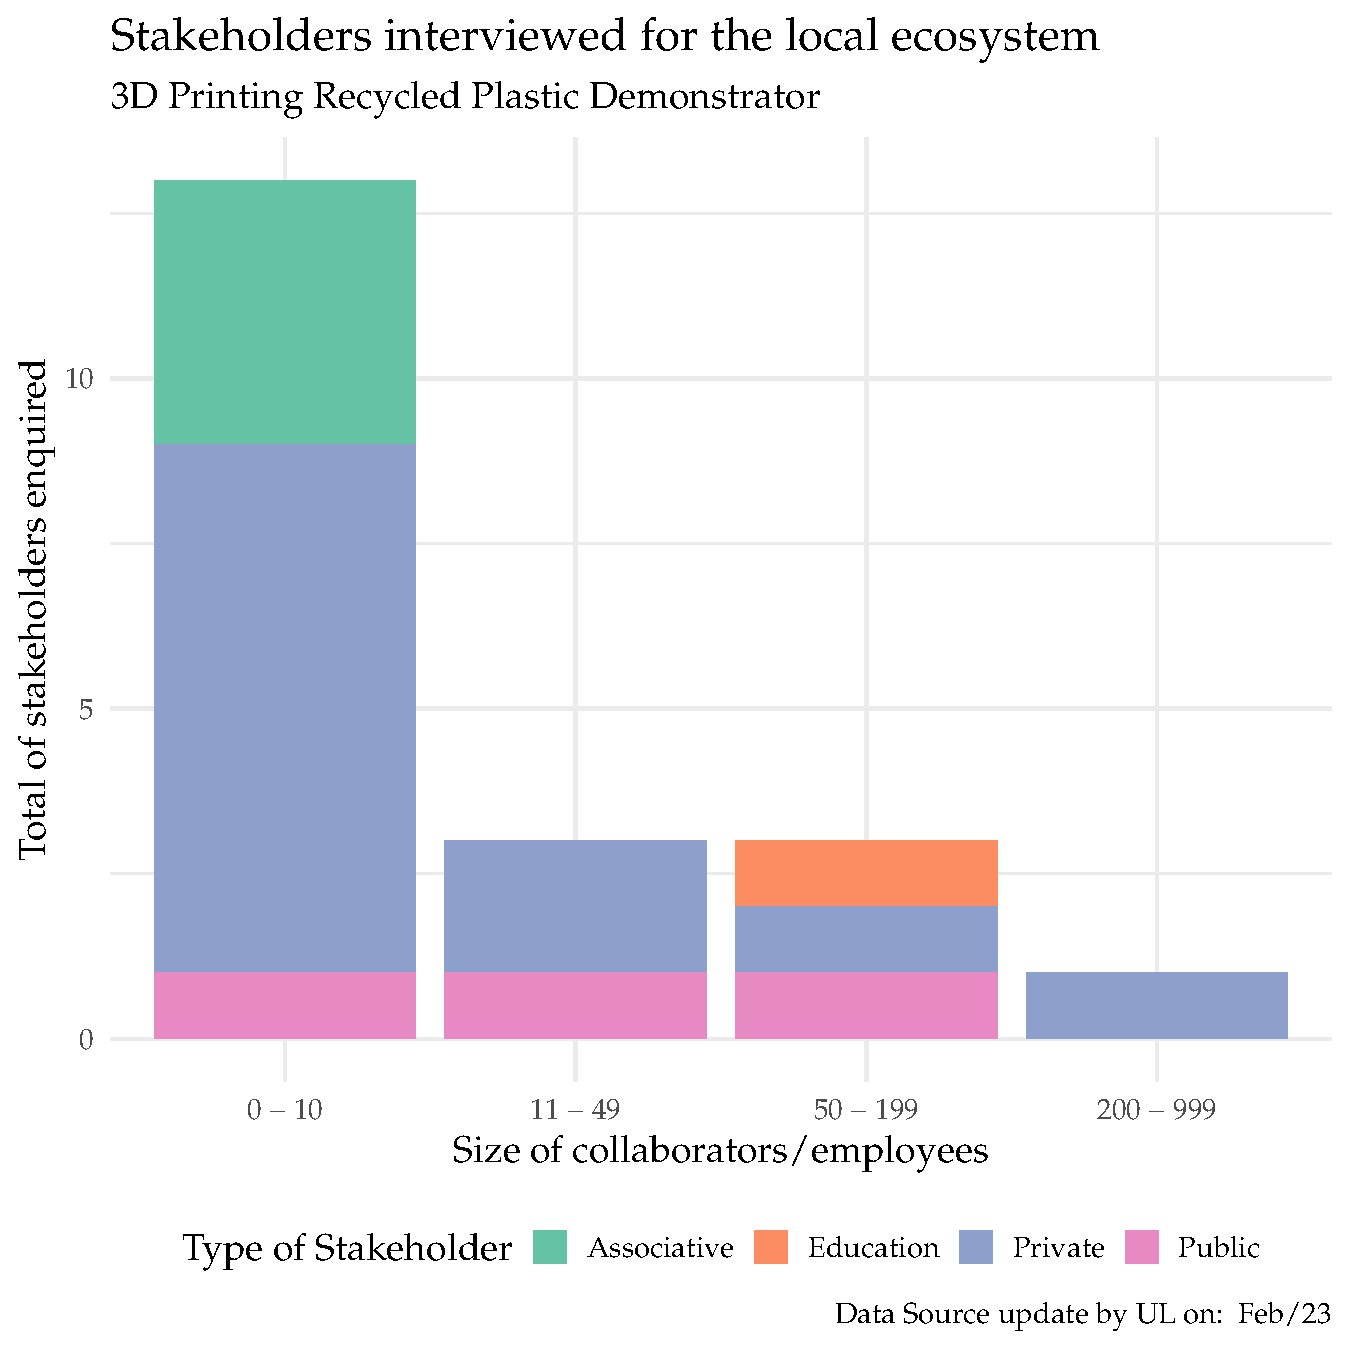
\includegraphics{figures/fedoua/Ecosystem-01.pdf}

}

\subcaption{\label{fig-ecosystem-00}Total of stakeholders}
\end{minipage}%
%
\begin{minipage}[b]{0.50\linewidth}

{\centering 

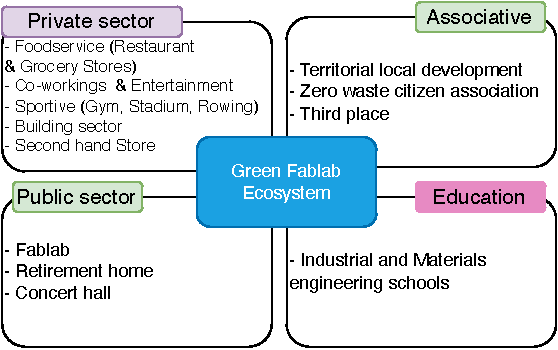
\includegraphics{figures/fedoua/Ecosystem-00.pdf}

}

\subcaption{\label{fig-ecosystem-01}Type of stakeholders addressed}
\end{minipage}%

\caption{\label{fig-ecosystem}Local ecosystem interviewed about the
implementation of 3D printing recycled demonstrator}

\end{figure}

A total of 23 actors were interviewed, of which 21 by physical or
telephone interview and 2 by electronic questionnaire. They were mainly
companies (47\% small and 26\% medium size), associative entities, and
the academic sector as displayed in the
Figure~\ref{fig-acceptability-01}. The diversity of the public was an
interesting criterion for the study. Participants in the economic,
cultural and social dynamics of the district through their membership in
the local association of economic actors of the territory were paped in
the Figure~\ref{fig-acceptability-02}

The scope of activity of most of the respondents is local (at the level
of the neighborhood or city) which may reflect a strong territorial
anchoring and a commitment to local concerns and issues (waste
management, social welfare, local job creation). The majority of their
business decisions are made locally, which reduces the risk of depending
on the interests of entities outside the territory.

\begin{figure}

\begin{minipage}[b]{0.50\linewidth}

{\centering 

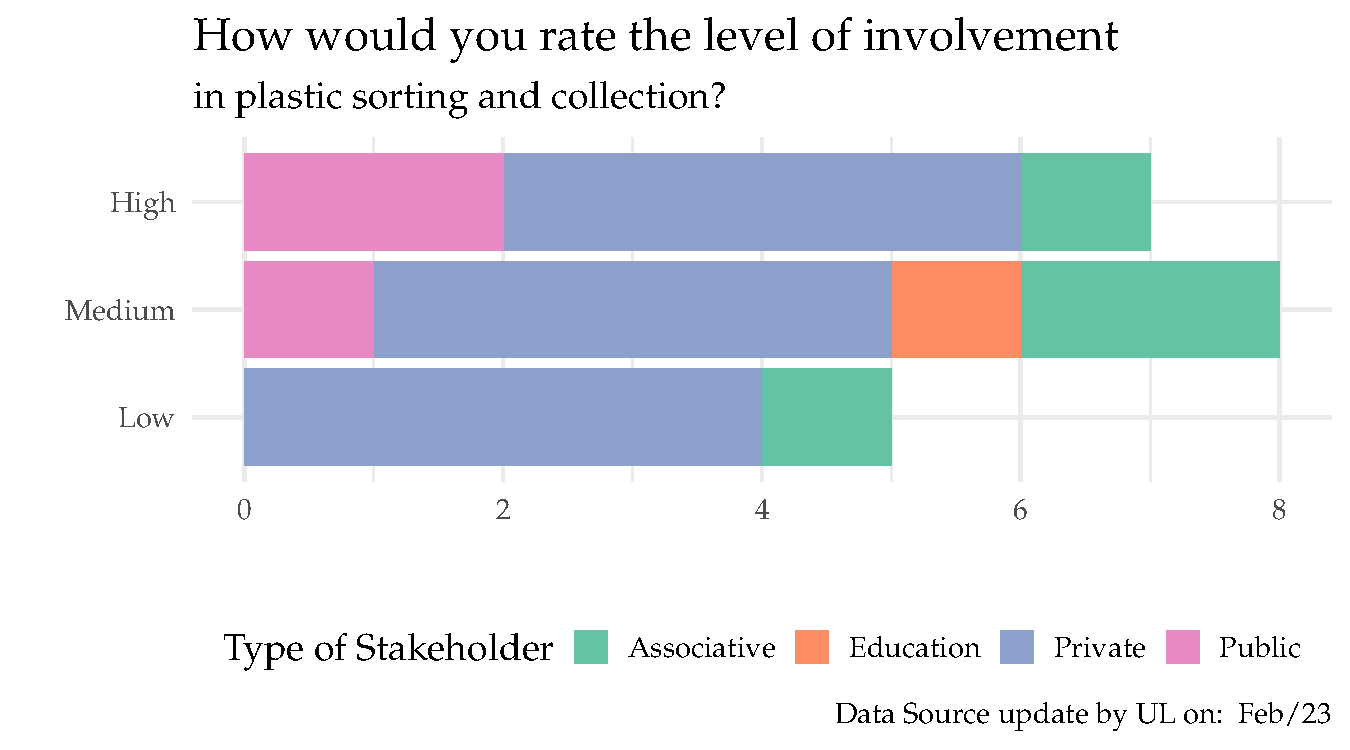
\includegraphics{figures/fedoua/Acceptability-01.pdf}

}

\subcaption{\label{fig-acceptability-01}Local ecosystem interviewed
about the implementation ofa 3D printing recycled demostrator}
\end{minipage}%
%
\begin{minipage}[b]{0.50\linewidth}

{\centering 

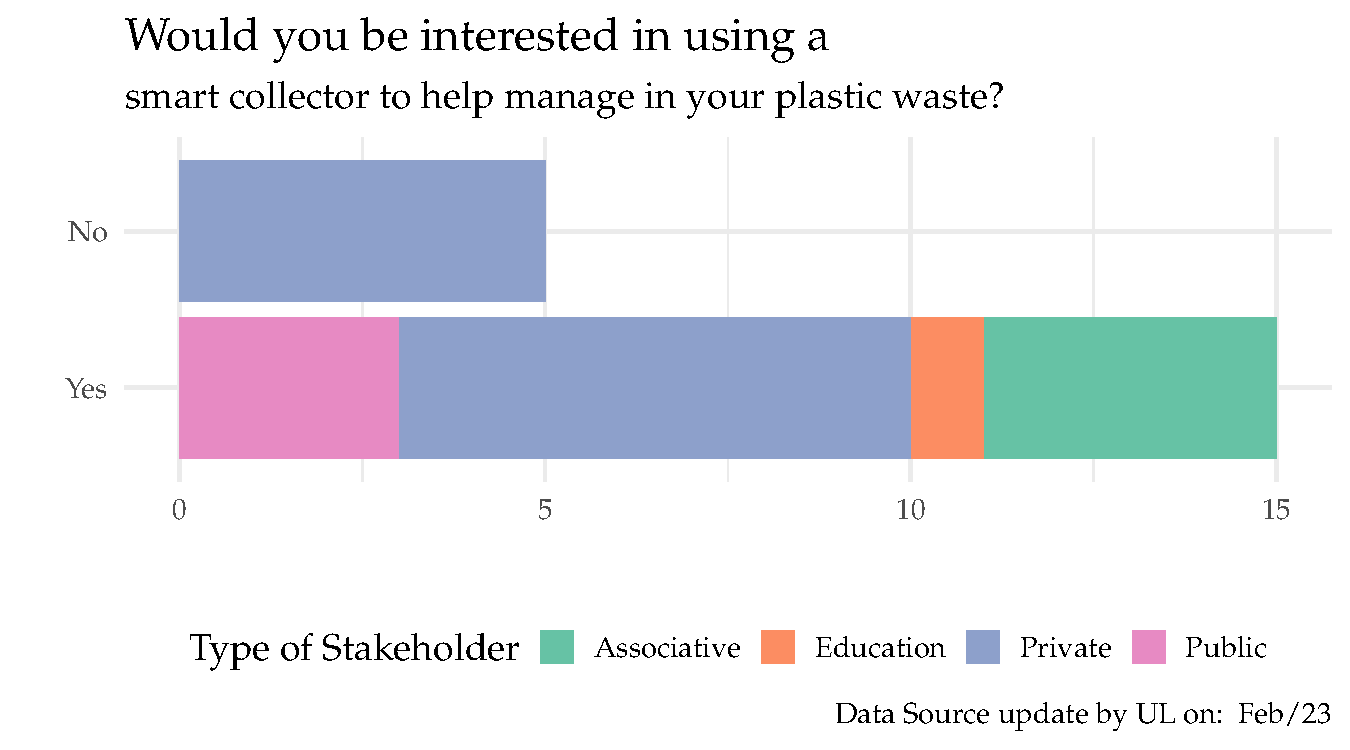
\includegraphics{figures/fedoua/Acceptability-02.pdf}

}

\subcaption{\label{fig-acceptability-02}Acceptability of the possible
use of `smart collector' for the}
\end{minipage}%

\caption{\label{fig-acceptability}Answers of the local ecosystem
enquired about the implementation of a through the smart collector
prototype}

\end{figure}

First, an inventory of their plastic waste practices was carried out.\\
The majority of the establishments surveyed generate plastic waste which
is mainly food waste (bottles and packaging). However, they do not all
have a specific system for the management of this waste, but above all
they sort glass and cardboard/paper. This can be explained by a lack of
internal resources, such as the absence of suitable materials for
sorting plastic, or the lack of dedicated skills (only 5 establishments
have staff in charge of waste management). In some cases, the sorting
process is not complete, as the sorted waste is mixed with other types
of waste at the time of collection due to a lack of awareness. Other
establishments depend on the system of public or private collection
companies, which limits their involvement in the management of this
plastic, and sometimes leads to a lack of information on what happens to
this waste after collection. The majority of respondents confirm that
they were favorable to participate in civic initiatives, to commit to
environmental protection and to participate in the dissemination of
these good practices to their local ecosystem.

When mentioning a smart collector to the interviewees, this means for
them a collector ``\emph{that does the sorting by itself}'' or a
technology that allows to ``\emph{count plastic waste on a territory
scale}''. These terms reflect a need for such equipment to help these
facilities manage their waste more easily, especially when most of them
do not have plastic-specific sorting equipment. Most of the interviewees
were motivated to receive one or more smart collectors: ``\emph{a large
quantity of plastic caps and bottles are available at our place}'',
``\emph{very good, we'll go for it!}'', ``\emph{why not all that goes in
the direction of the improvement of daily life\ldots{}}''. However,
these comments are accompanied by some fears such as the difficulty in
managing the external public to respect the material, that other waste
is mixed with plastic, or the need to take the time to explain the
approach to the internal and external people of the institutions. The
minority refused to receive a smart collector or to participate in the
experimentation. The stated reasons and constraints such as the low
frequentation of the building, the lack of time to manage such an
approach, the need to have a consensus at the level of all the occupants
decision-makers of the building, lack of visibility on the technique, or
by personal conviction (e.g.~``\emph{I am not too electronic and
assisted, I like it when people manage by themselves}'').

Based on these insights, we could make a mapping of the role of each
actor that could have in the recovery process. Secondly, we identified
the sources of plastic waste collection, and then identified the sources
of 3D printing and potential synergies with the Green Fablab.

\hypertarget{step-4-put-in-place-smart-collectors}{%
\subsection{Step 4: Put in place smart
collectors}\label{step-4-put-in-place-smart-collectors}}

Thanks to the step 3, we have identified the collection sites at the
local territory for the deployment of the smart collector. In this step
the main purpose was the deployment of a set of \emph{smart collectors}
around the neighborhood. Figure~\ref{fig-sc-deployment} presents the
selected points around the Green FabLab for the installation of the
prototype. The smart collector is produced and mounted manually at Green
FabLab facilities. The specific details and step-by-step assemble
process can be found in the technical paper
(\protect\hyperlink{ref-gabriel2023}{Gabriel and Cruz, 2023}).

\begin{figure}[H]

{\centering 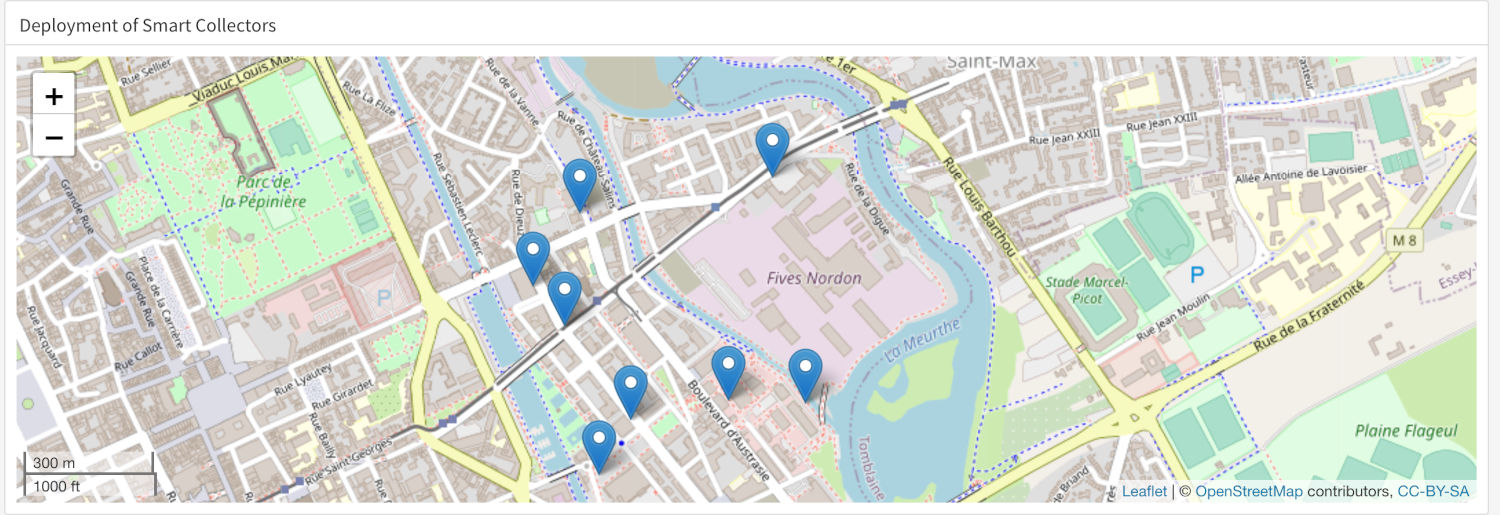
\includegraphics[width=6.25in,height=\textheight]{figures/SC/Deployment.jpg}

}

\caption{\label{fig-sc-deployment}Deployment of the Smart Collectors.}

\end{figure}

The selection of the places were based on the steps 3. For the
experimentation, eight sites were selected for the deployment as listed
in the Table~\ref{tbl-deployment}.

\hypertarget{tbl-deployment}{}
\begin{table}[H]
\caption{\label{tbl-deployment}Selected points of deployment of the smart collector in the
neighboorhood of Rives de Meurthe, Nancy - France. }\tabularnewline

\centering\begingroup\fontsize{10}{12}\selectfont

\begin{tabular}[t]{r>{\raggedright\arraybackslash}p{3cm}l>{\raggedright\arraybackslash}p{5cm}}
\toprule
ID & Type​ & Potential public​ & Main activity\\
\midrule
\cellcolor{gray!6}{1} & \cellcolor{gray!6}{Association​ } & \cellcolor{gray!6}{+300​ } & \cellcolor{gray!6}{Cultural/leisure activities}\\
2 & Association ​  & +1000​  & Third place, Co-working space\\
\cellcolor{gray!6}{3} & \cellcolor{gray!6}{Private Entreprise​ } & \cellcolor{gray!6}{+100​ } & \cellcolor{gray!6}{Sport Gym}\\
4 & University  & 300​  & Engineering school\\
\cellcolor{gray!6}{5} & \cellcolor{gray!6}{Private Enterprise} & \cellcolor{gray!6}{50​ } & \cellcolor{gray!6}{Mutual Insurance}\\
\addlinespace
6 & University  & 500​  & Engineering school\\
\cellcolor{gray!6}{7} & \cellcolor{gray!6}{Public Entreprise​ } & \cellcolor{gray!6}{50​ } & \cellcolor{gray!6}{Management of waterrways network}\\
8 & Association​  & +100​  & Sports club (Rowing)\\
\bottomrule
\end{tabular}
\endgroup{}
\end{table}

First, face-to-face meetings with the local actors were made to obtain
the agreement for the installation of the prototype. As a relevant
criteria, the installation needed to be in a location were the
visitors/employees/customers of the selected point are able to see the
device. We designed an appropriate communication that enables to explain
the purpose of the device and connect to the information of INEDIT
projet (see Figure~\ref{fig-smart})

\begin{figure}

\begin{minipage}[b]{0.50\linewidth}

{\centering 

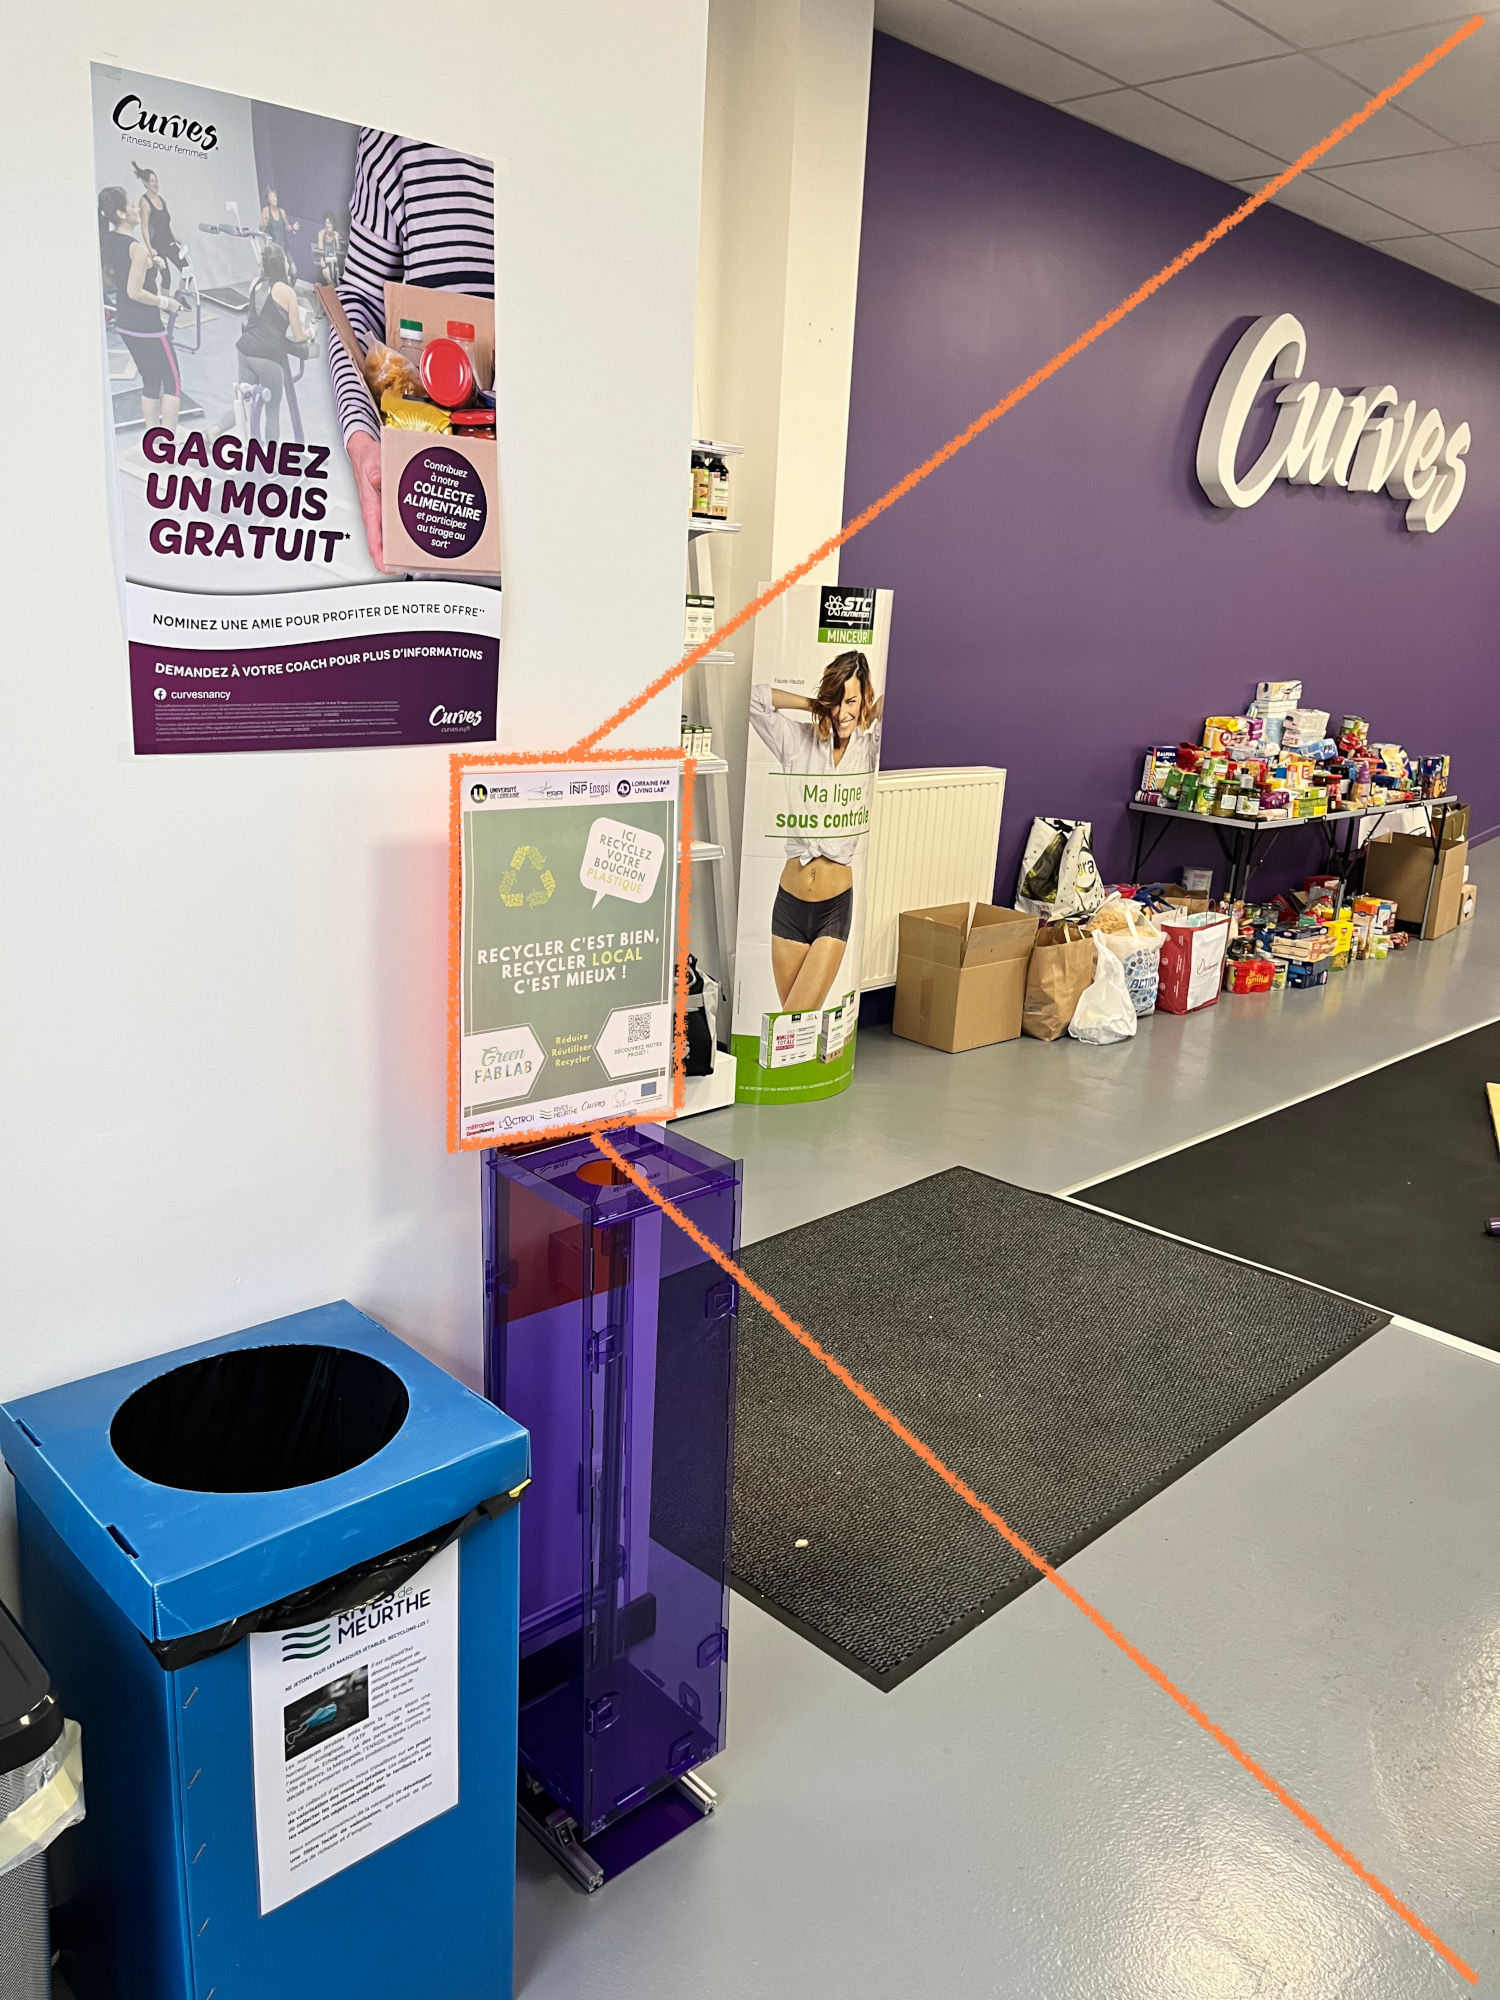
\includegraphics[width=2.5in,height=\textheight]{figures/SC/curves-00.jpeg}

}

\subcaption{\label{fig-sc-curves}Smart collector at the collection
point}
\end{minipage}%
%
\begin{minipage}[b]{0.50\linewidth}

{\centering 

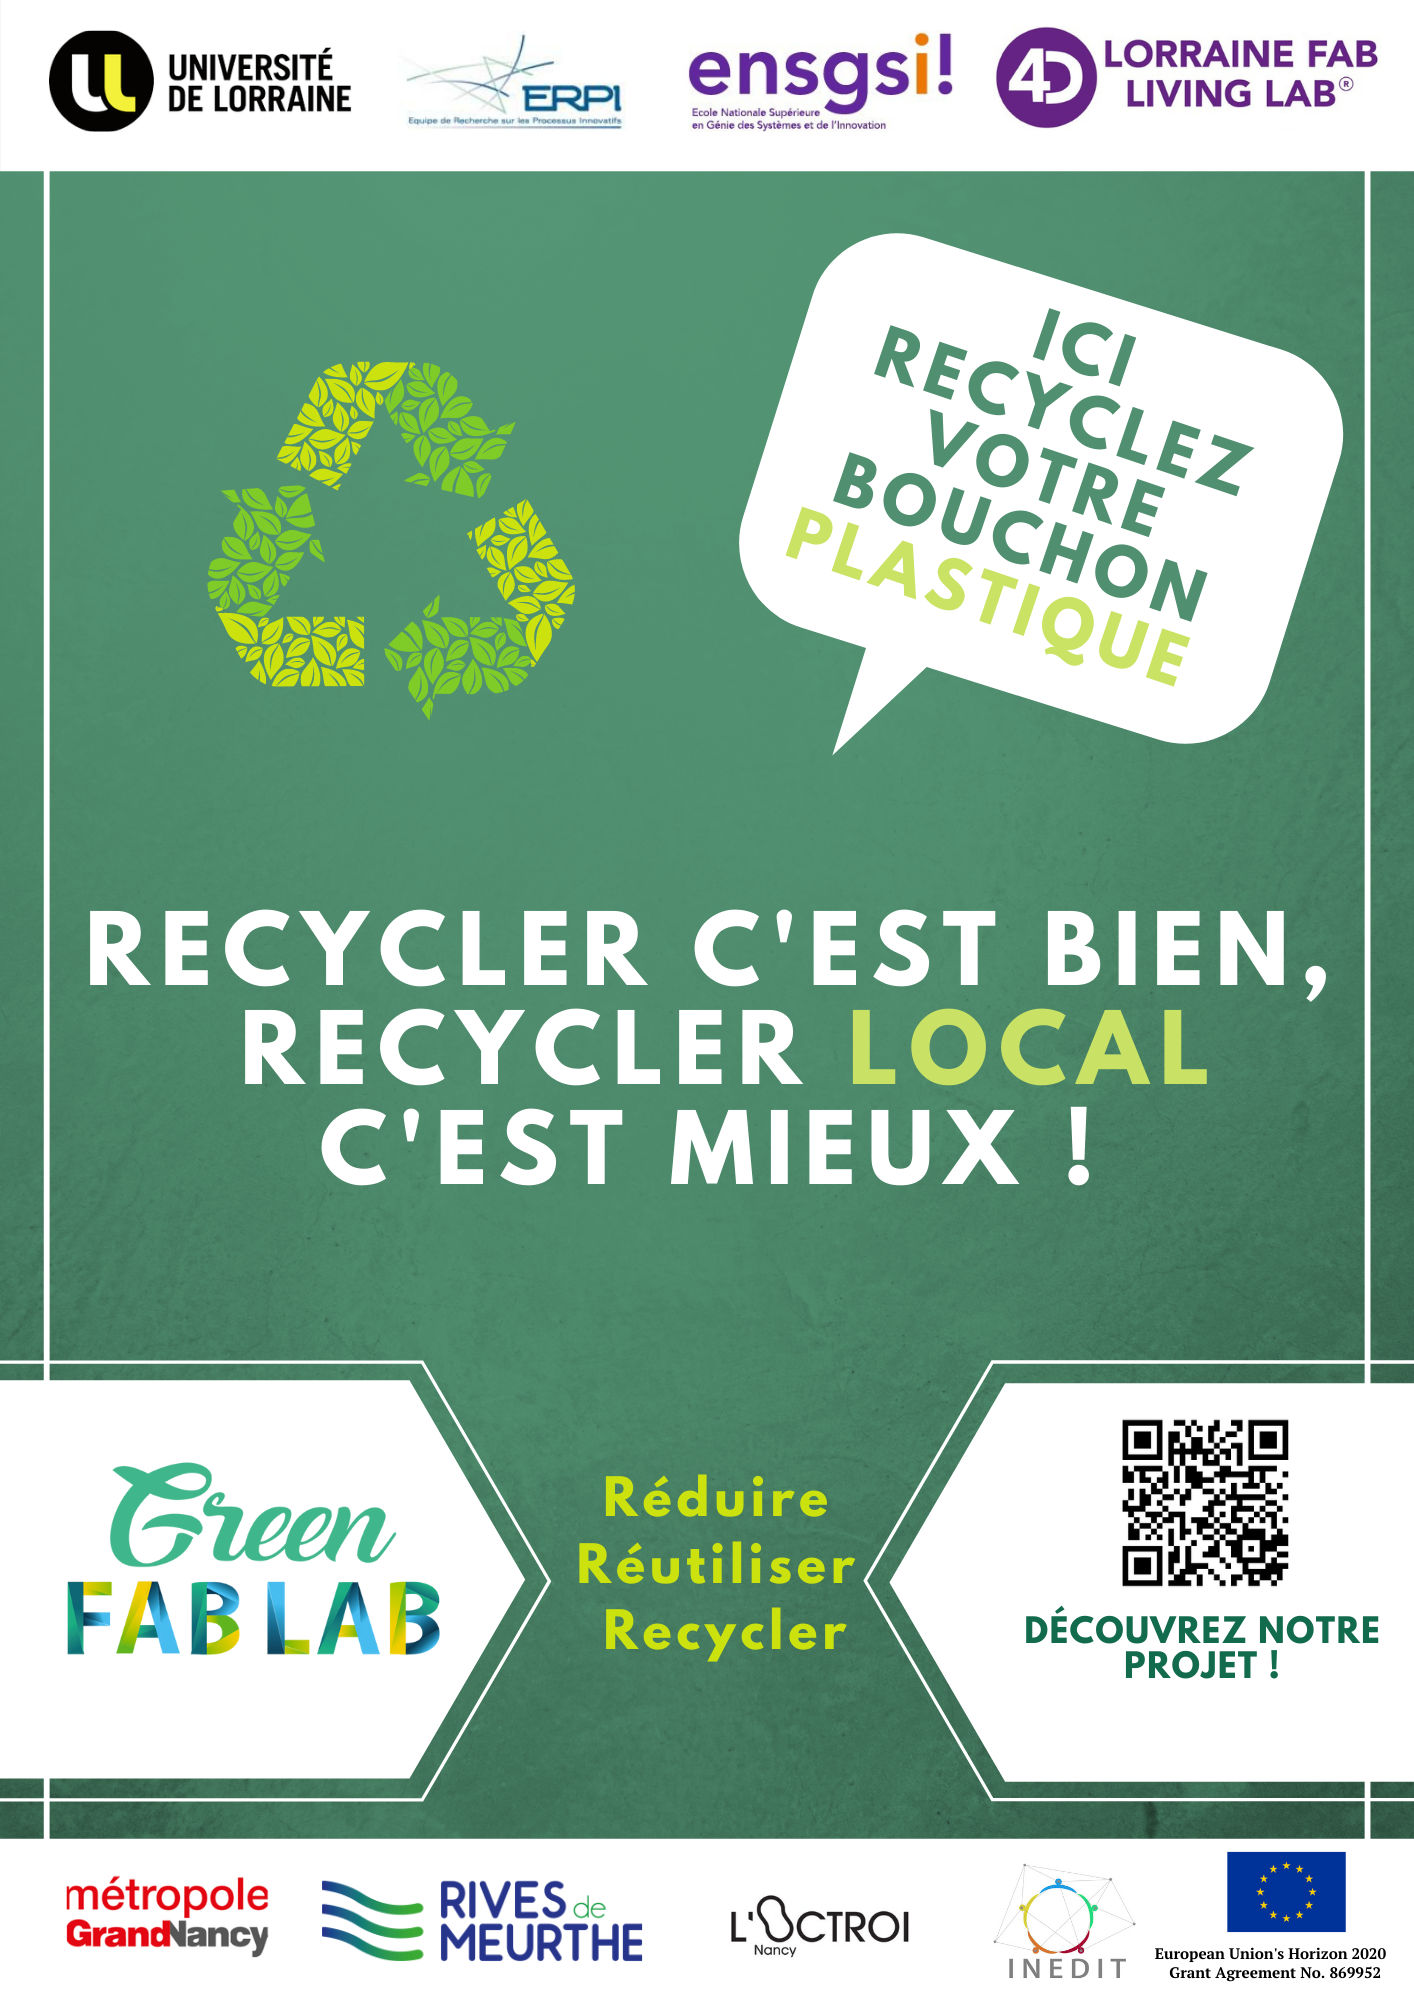
\includegraphics[width=2.5in,height=\textheight]{figures/SC/comm.jpg}

}

\subcaption{\label{fig-sc-flyer}Communication strategy of the device}
\end{minipage}%

\caption{\label{fig-smart}Deployment example of the smart collector at
the collection point}

\end{figure}

Then, a system activation is putted in place to begin the collection
gate. Once the smart collector is online, it is necessary to survey the
online dashboard to control the waste plastic quantity. In the moment
that the dashboard present a weight more than 3 kg, we mapped the
collection point in the stage of \emph{`to collect'} and we plan the
recovery. The distance of the collection place is less than \(2~km\) so
is carried out by bicycle or on foot to avoid the possible impact
produced for a combustion or electric vehicle.

\begin{figure}[H]

{\centering 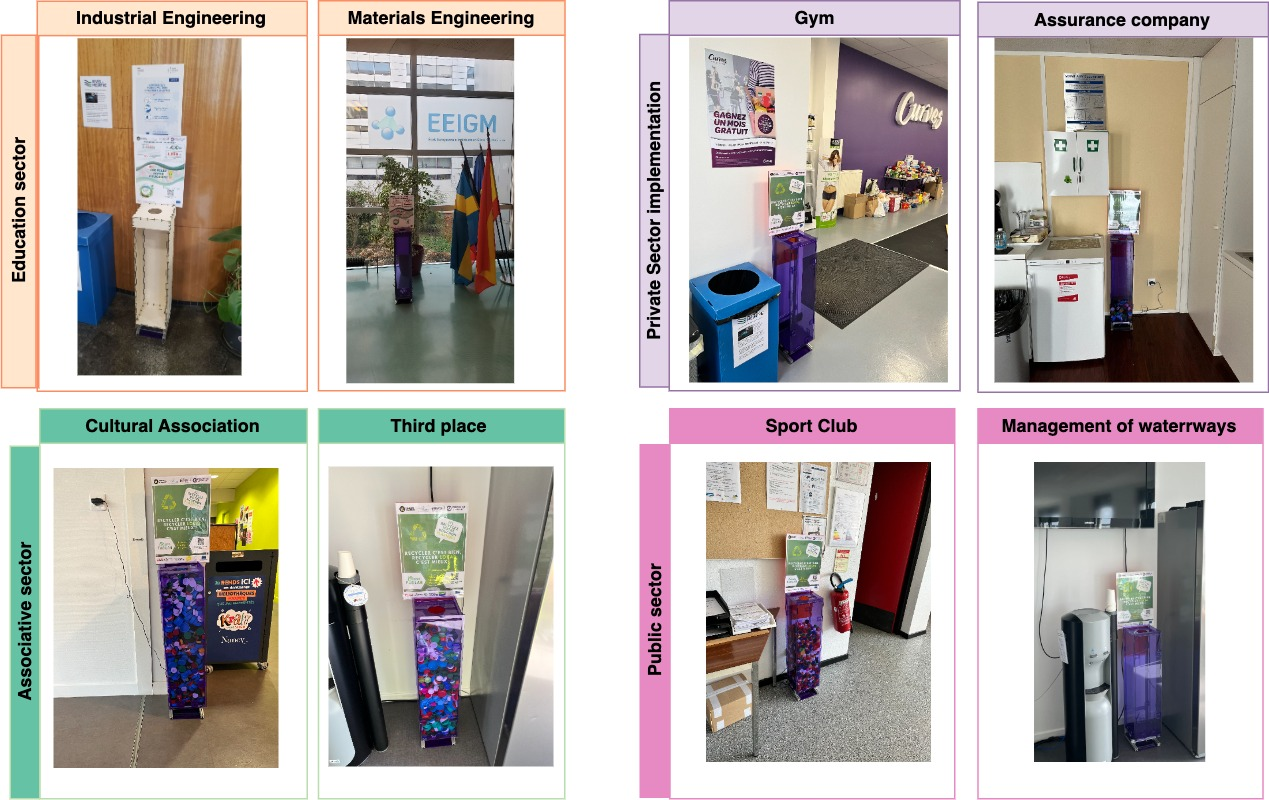
\includegraphics[width=0.9\textwidth,height=\textheight]{figures/SC/Smart-Collectors.jpg}

}

\caption{\label{fig-sc-flyer}Smart collectors deployed in the territory}

\end{figure}

\hypertarget{step-5-transport-waste-material-to-the-recycling-facilities}{%
\subsection{Step 5: Transport waste material to the recycling
facilities}\label{step-5-transport-waste-material-to-the-recycling-facilities}}

The recovery process took place once a week on average. When the waste
plastic is collected, it is stored at the facilities of the Green
FabaLab before posterior treatment and adequation.\\
We have build a central collector as illustrated by the figure
Figure~\ref{fig-sc-recovery} where the material is stored before it is
treated.

\begin{figure}

\begin{minipage}[b]{0.50\linewidth}

{\centering 

\includegraphics[width=2in,height=\textheight]{figures/SC/Collector-bouchons-00.jpeg}

}

\subcaption{\label{fig-sc-collector-00}Central storage of plastic waste}
\end{minipage}%
%
\begin{minipage}[b]{0.50\linewidth}

{\centering 

\includegraphics[width=2in,height=\textheight]{figures/SC/Collector-bouchons-01.jpeg}

}

\subcaption{\label{fig-sc-collector-01}Communication flyer for the smart
collector}
\end{minipage}%

\caption{\label{fig-sc-collector}Central storage of the collected
plastic waste.}

\end{figure}

Throughout the experimentation of the deployment, we have mapped the
quantity of collected material. Figure~\ref{fig-sc-recovery} corresponds
to the profile of quantity collection per month. In average, we have
collected 3kg per week.

\begin{figure}[H]

{\centering 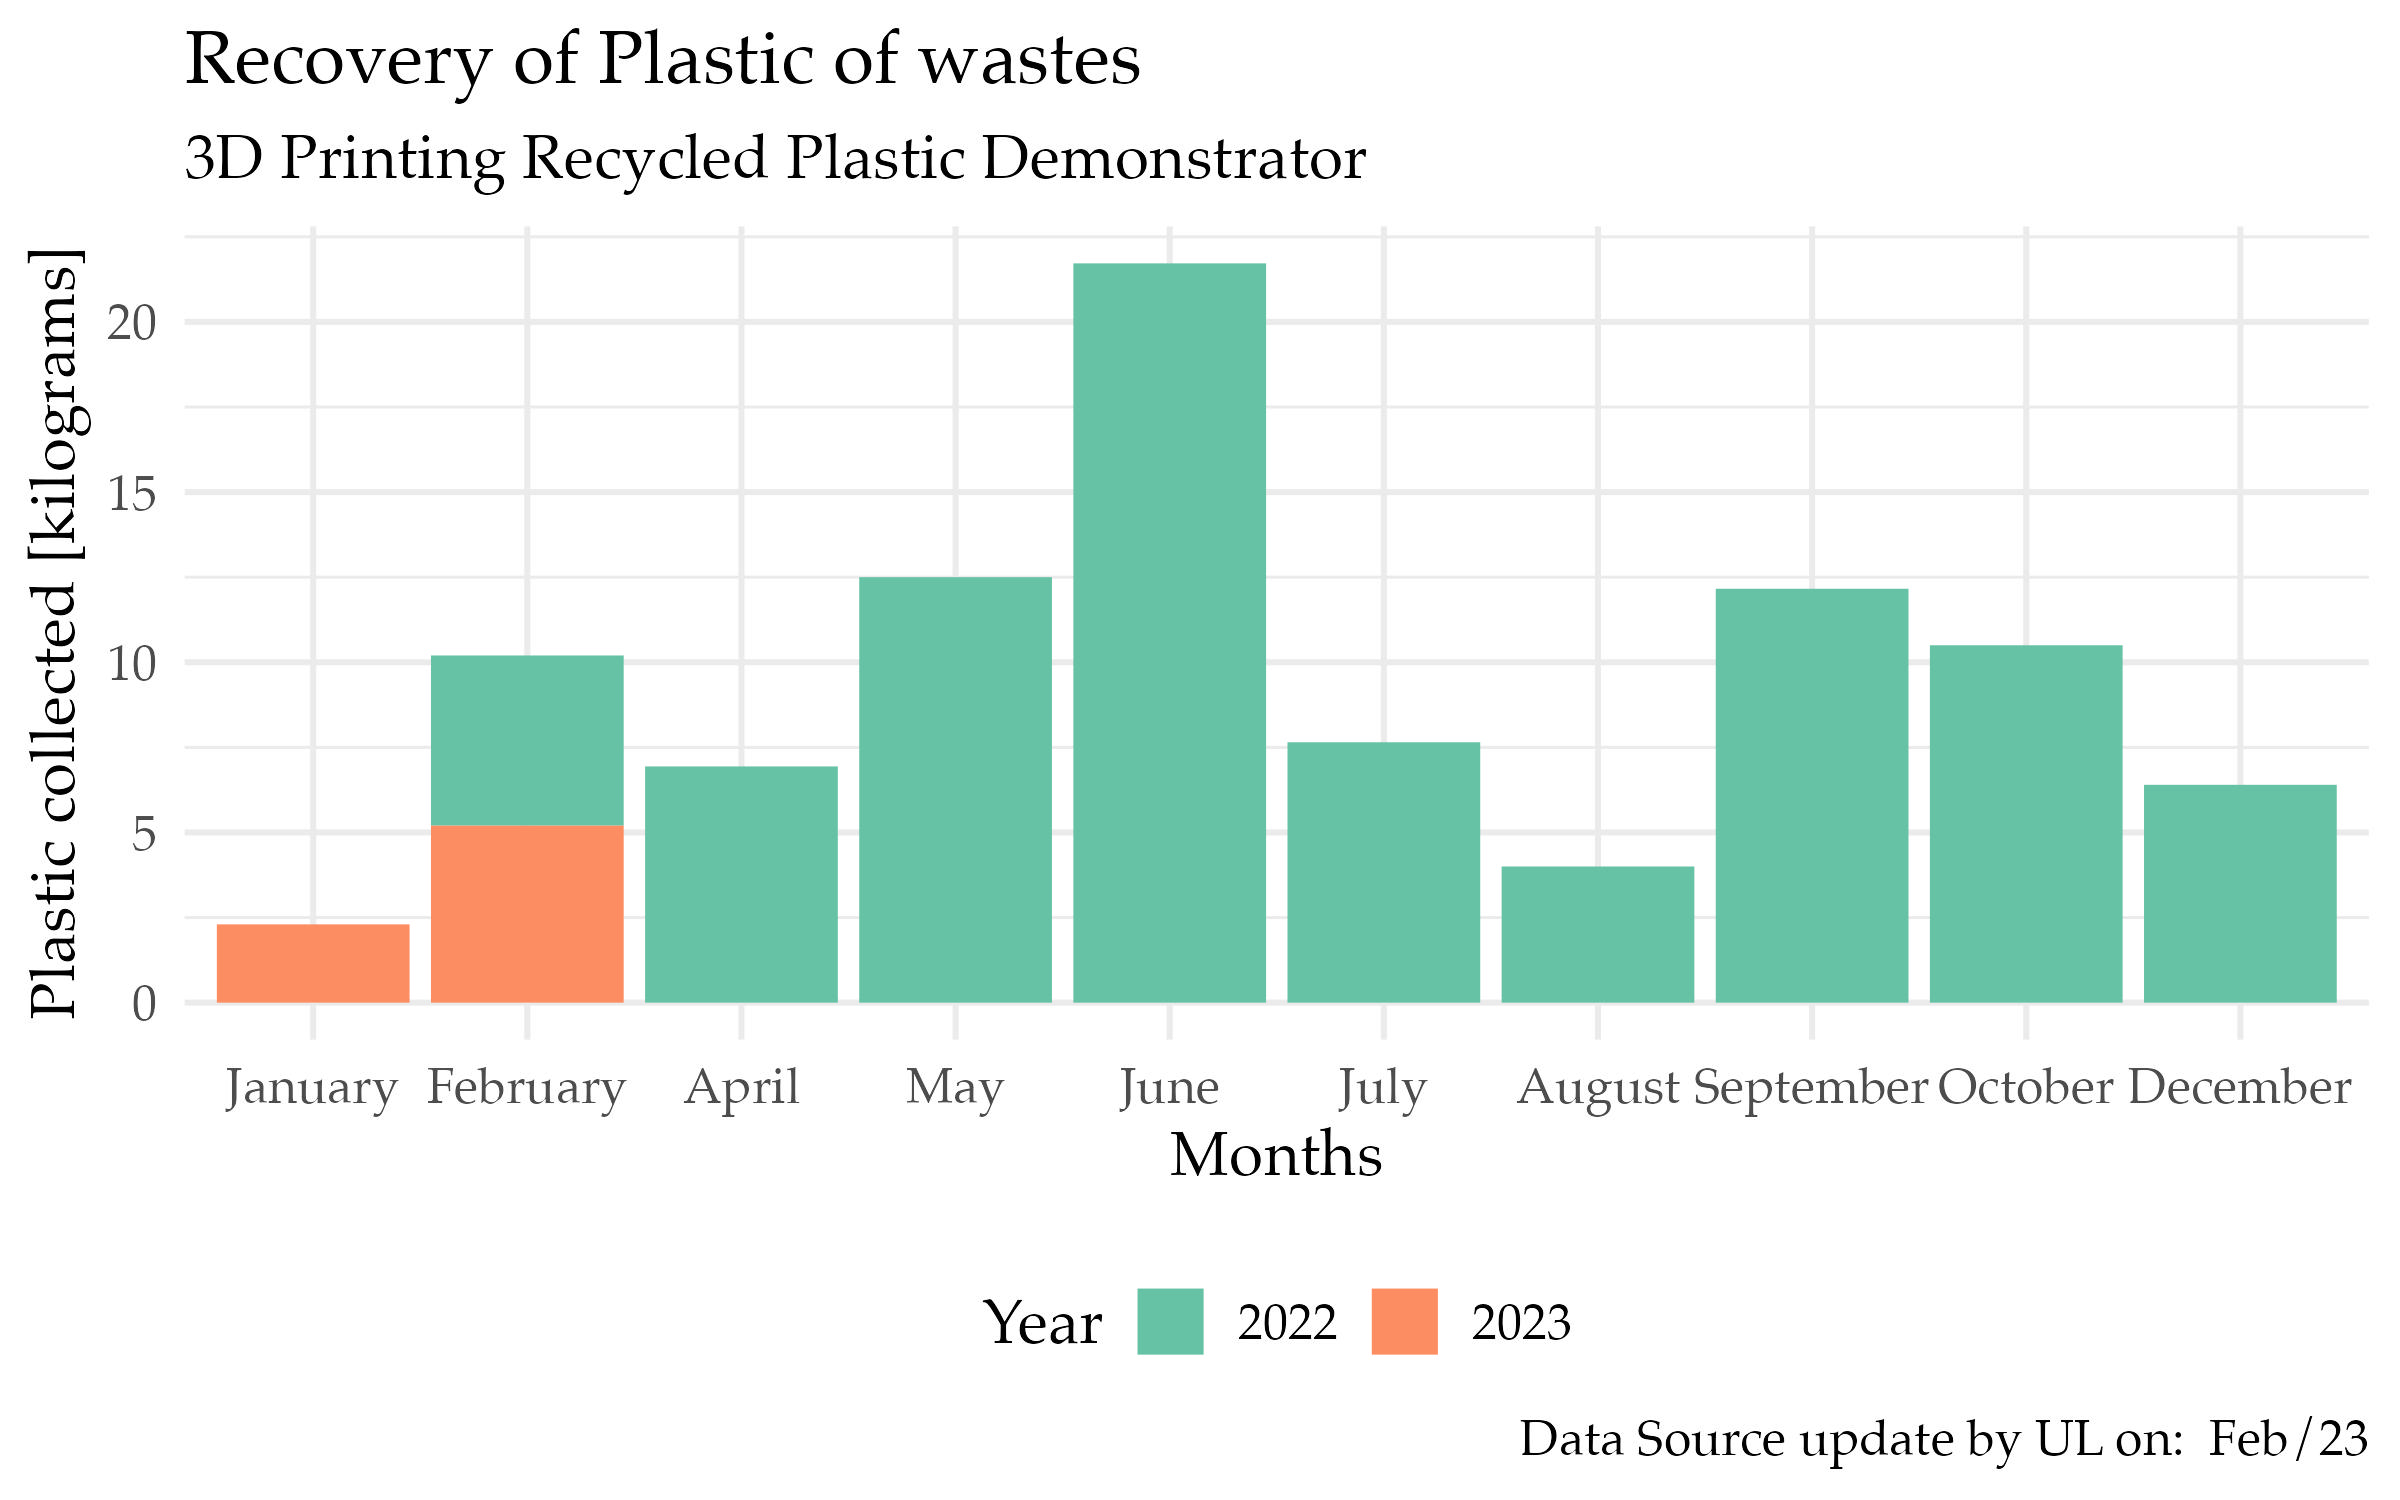
\includegraphics[width=0.7\textwidth,height=\textheight]{figures/SC/Recovery.jpg}

}

\caption{\label{fig-sc-recovery}Recovery profile of plastic}

\end{figure}

\begin{tcolorbox}[enhanced jigsaw, rightrule=.15mm, coltitle=black, breakable, bottomtitle=1mm, title=\textcolor{quarto-callout-note-color}{\faInfo}\hspace{0.5em}{Key Performance Indicator of the Recovery process}, titlerule=0mm, opacitybacktitle=0.6, opacityback=0, colframe=quarto-callout-note-color-frame, arc=.35mm, toprule=.15mm, leftrule=.75mm, colbacktitle=quarto-callout-note-color!10!white, toptitle=1mm, left=2mm, colback=white, bottomrule=.15mm]

In terms of \emph{KPI} of the recovery, from February 2022 to February
2023, we have collected a total of \(94.37~kg\) of plastic waste using 8
collectors in the territory of Rives de Meurthe, Nancy-France.

\end{tcolorbox}

\hypertarget{step-6-adequation-and-preparation-of-the-material}{%
\subsection{Step 6: Adequation and preparation of the
material}\label{step-6-adequation-and-preparation-of-the-material}}

This is the first stage carried out inside the Green Fablab. This stage
corresponds to the set of activities required for the plastic waste to
be adapted for further use. The Green Fablab works mainly with 4 types
of plastic at the moment. The most common are high density polyethylene
(HDPE) and polypropylene (PP), which are the main plastics used in the
production of bottle caps and they are collected in the smart collector.
The plastic waste from unused/damaged 3D printing parts mainly of
polylactic acid (PLA) are collected mainly from the Lorraine Fab Living
Lab. And finally, the plastic bottles also are collected which are
polyethylene terephthalate (PET).

The preparation process begins with the separation and identification of
each plastic collected. As already mentioned, the plastics used in the
Green FabLab are 4 (HDPE, PP, PET and PLA) and are separated by type of
plastic and color. This process is carried out manually.

\begin{figure}[H]

{\centering 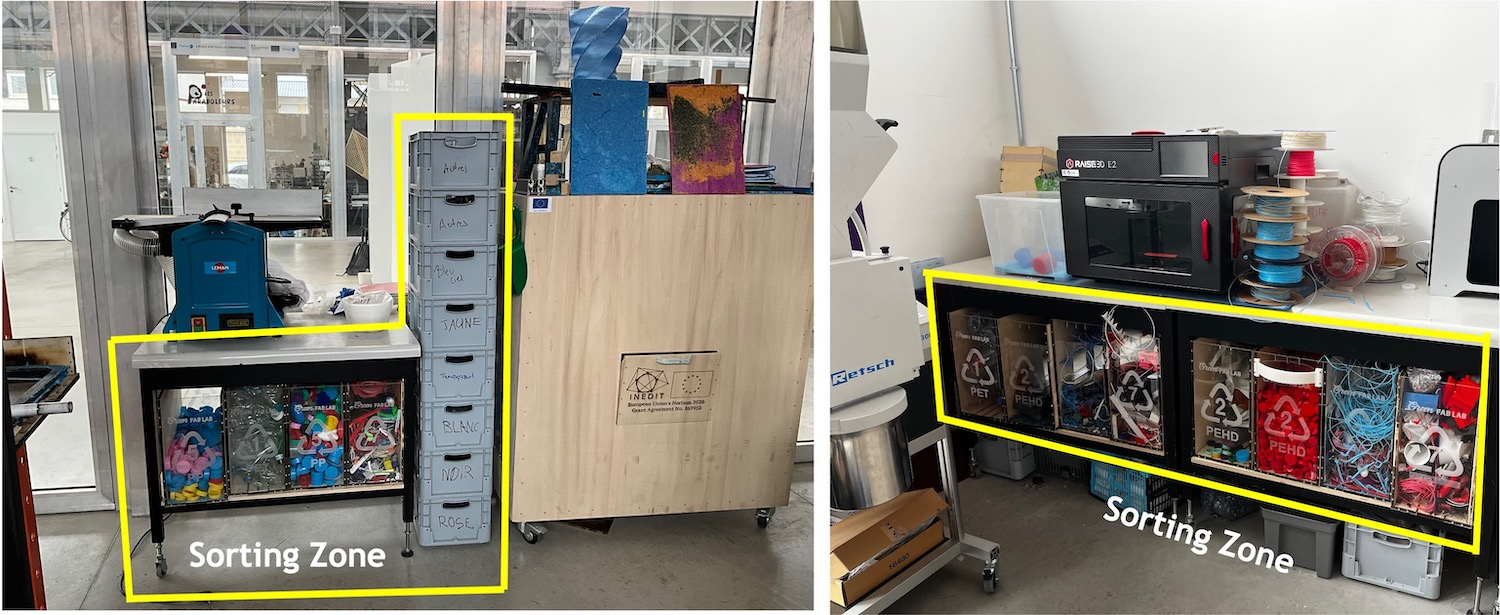
\includegraphics[width=0.9\textwidth,height=\textheight]{figures/preparation/sorting-2.jpg}

}

\caption{Sorting process of the plastic cups in function of the type of
plastic accordig to the standard identification}

\end{figure}

The second step is the cleaning phase. Cleaning and washing plastic cups
and bottles is a crucial step for effective recycling. Plastics are
mainly post-consumer waste, thus they are not in an adequate state of
cleanliness to be introduced in the technical machines. It is required
to ensure the plastic is as clean as possible because dirty material can
affect the quality of the extrusion / printing process, which at the end
affects the recycled product. Therefore, we aim to remove adhesives,
leftover waste, and labels. HDPE and PP are mainly used in the plastic
injection molding process, while PLA and PET (Mixed with 9\% HDPE) are
used in 3D printing.

\begin{figure}[H]

{\centering 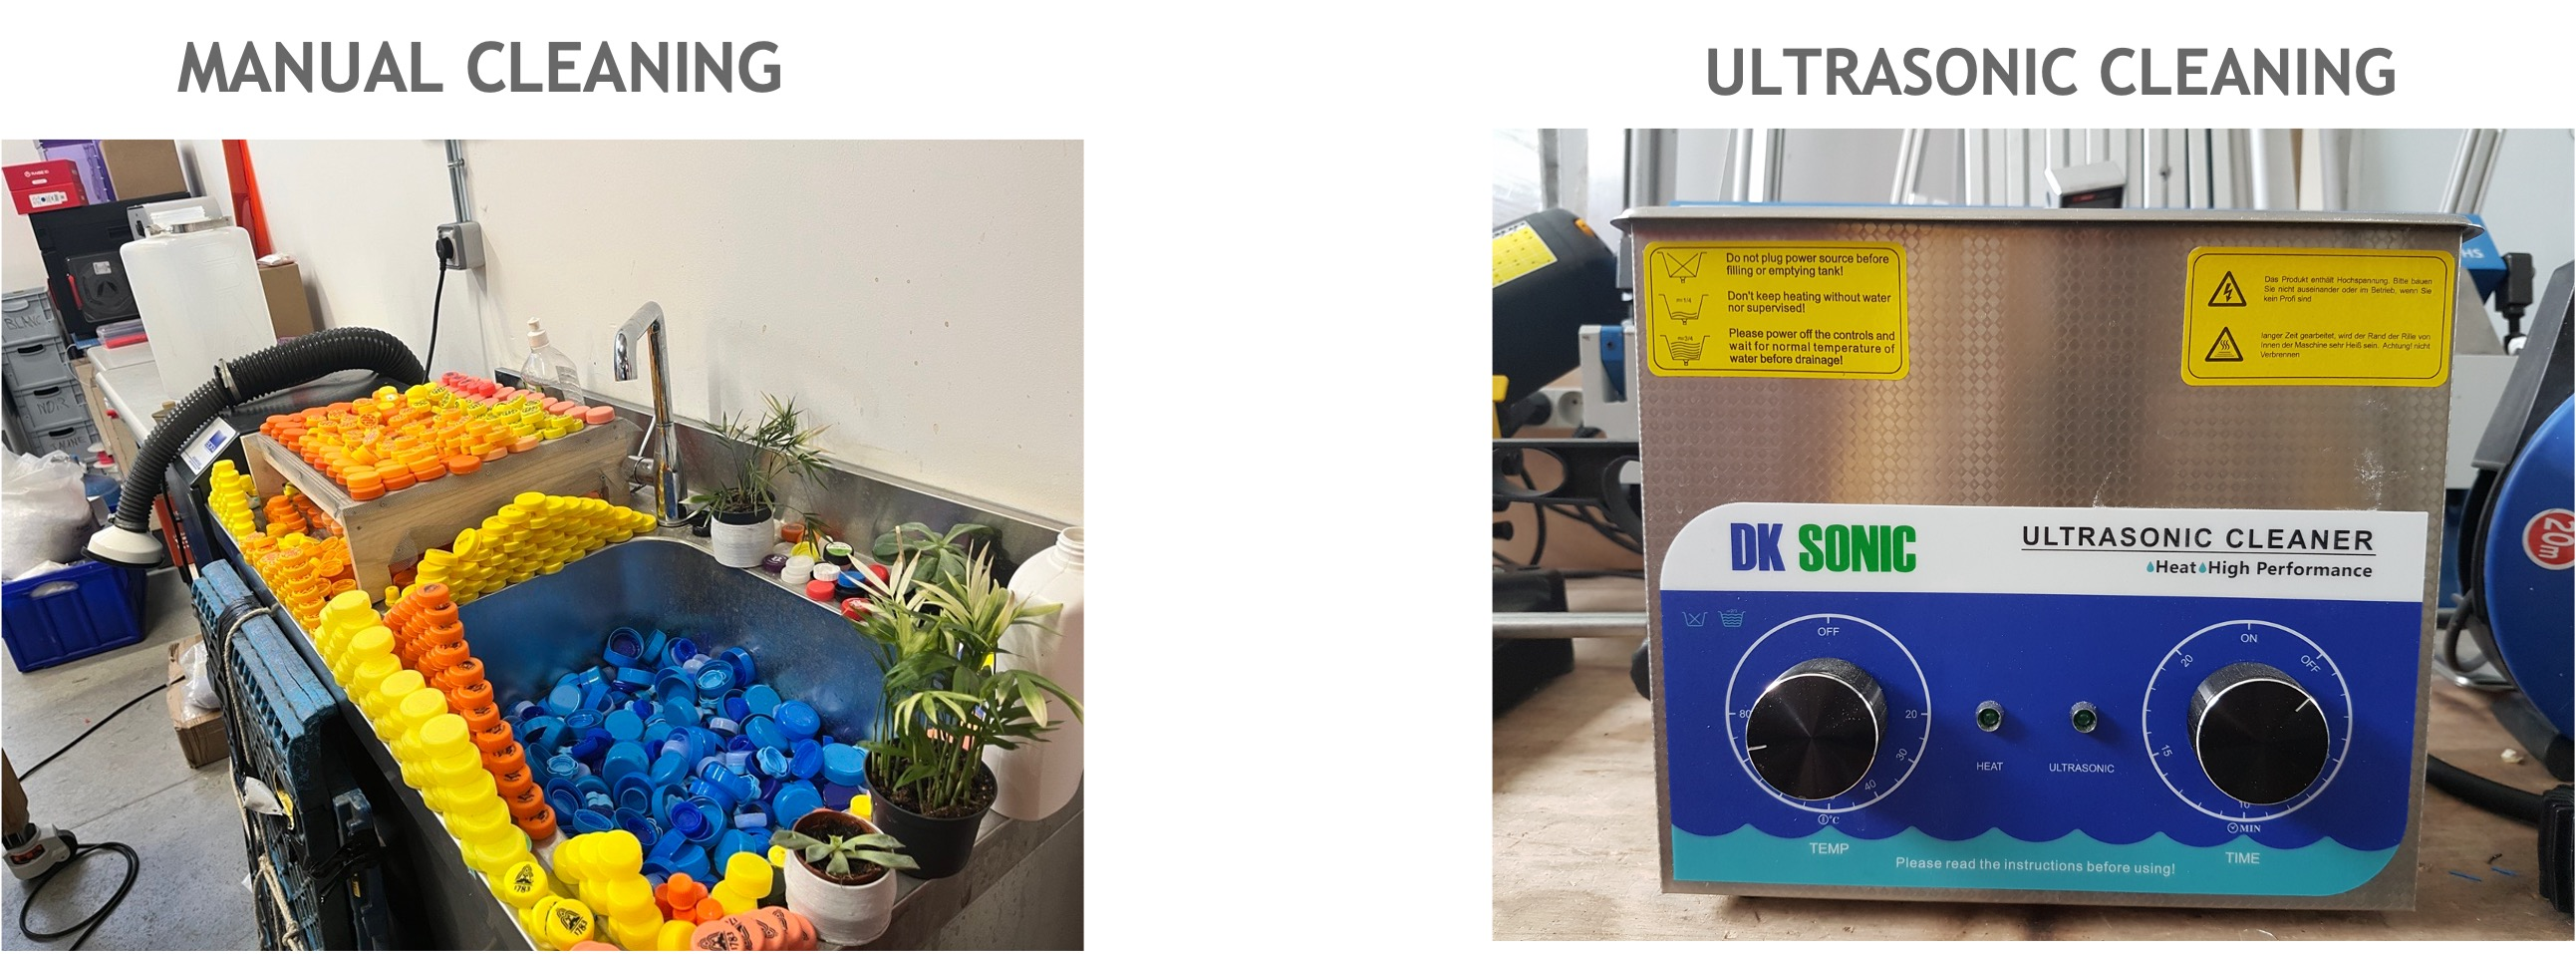
\includegraphics[width=0.7\textwidth,height=\textheight]{figures/cleaning/cleanning.jpg}

}

\caption{Manual and ultrasonic cleaning processes}

\end{figure}

In the first moment, the manual cleaning is used to remove most of the
major contaminants present in the material. For plastic injection
molding, where mainly PP and HDPE are used, the plastic is washed in a
sink with hot water.\\
The water consumption per gram is approximately 4 liters per kilogram.
The drying of the plastic is done by natural convection in the open air.

For additive manufacturing, where mainly PLA, HDPE and PET blends are
used, the cleaning process is much more controlled. The process is
carried out in a small ultrasonic cleaning machine, to ensure that
impurities are removed. The cleaner ultrasonic machine washes 200 gr of
plastic with 1 L of water.. This process takes 20 mins with a
consumption of 2kWh.

The second step in the preparation of the waste material is the size
reduction process. In this step, the washed and sorted plastic is sent
through a shredding machine where it is grounded into smaller pieces of
plastic. A critical parameter in the control of the granulometry. The
purpose of the size reduction is to obtain plastic waste where the
granulometry corresponds to the extrusion / printing. The plastic waste
needs to be reduced from a range of between 25-50 mm to 3-5mm
approximately after grinding. A cutting mill machine SM 300
Retsch\textsuperscript{\textregistered} with a selectable speed range
from 700 to 3,000 \(rpm\) was used. The selected speed was \(1500~rpm\).
Normally we use a rotational speed of 1500 which produces an energy
consumption of 0.7 kWh. The process takes 15 minutes per kilogram of
material with a loss of approximately 10\%. Therefore, after shredding
it is necessary to sieve to identify the optimum size.

\begin{figure}[H]

{\centering 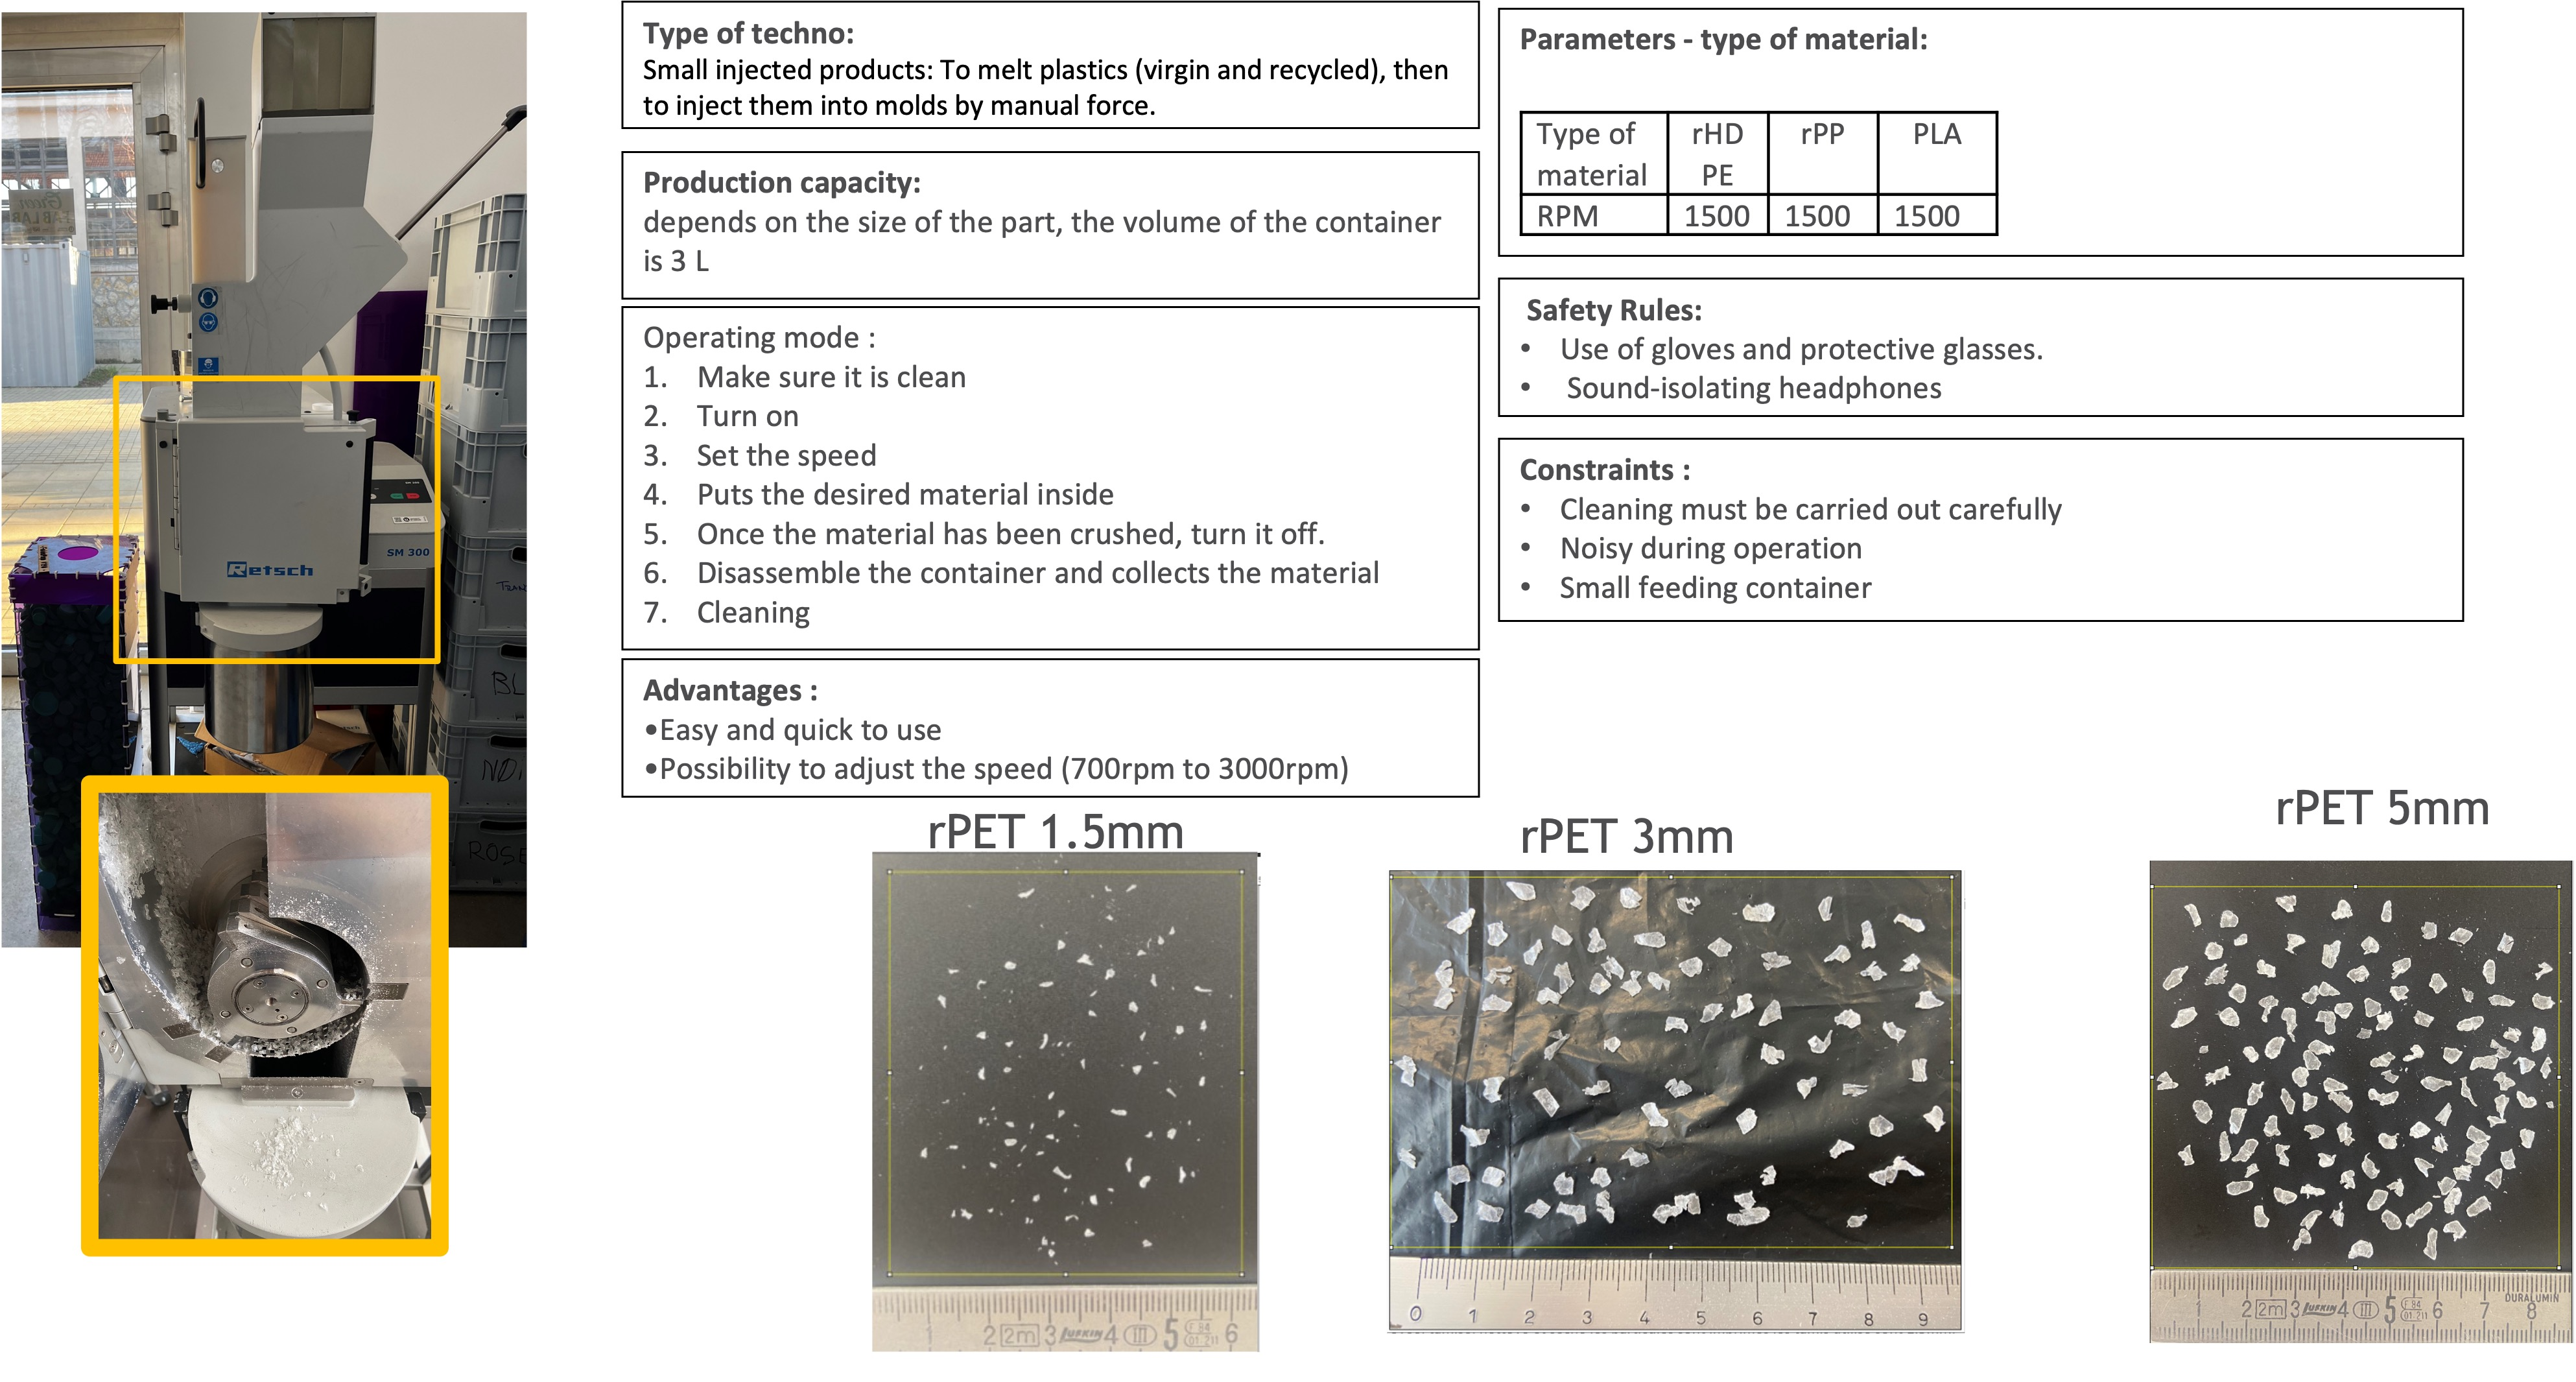
\includegraphics[width=6.25in,height=\textheight]{figures/shredding/shreeding.jpg}

}

\caption{Photo of the Shredding process}

\end{figure}

\begin{tcolorbox}[enhanced jigsaw, rightrule=.15mm, coltitle=black, breakable, bottomtitle=1mm, title=\textcolor{quarto-callout-note-color}{\faInfo}\hspace{0.5em}{Key Performance Indicator of the FGF}, titlerule=0mm, opacitybacktitle=0.6, opacityback=0, colframe=quarto-callout-note-color-frame, arc=.35mm, toprule=.15mm, leftrule=.75mm, colbacktitle=quarto-callout-note-color!10!white, toptitle=1mm, left=2mm, colback=white, bottomrule=.15mm]

For fused granular fabrication technology, the optimum size for the
granulometry for printing is between 3 and 5mm. In terms of plastic
injection molding, the plastic flakes can be slightly larger than those
required for 3D printing.

\end{tcolorbox}

Finally, the drying process is the last step to prepare the material. To
remove all the moisture from the plastic it is necessary to carry out a
drying process in a conventional oven. In the drying phase, the plastic
is put in the oven at 60°C during 15h with a consumption of 0,061 Kwh.

\hypertarget{step-7-path-planning---3d-printing}{%
\subsection{Step 7: Path planning - 3D
Printing}\label{step-7-path-planning---3d-printing}}

In this step, the main purpose is to use the open source SuperSlicer
software, to establish the printing parameters considered for the
pieces. An experimental work needs to be made in order to adapt the
adequate configuration of the slicer with hardware of the Gigabot X and
FFF machines. Figure~\ref{fig-gcode} gives an overview of the
characteristics and basic parameters configurations considered in the
process.

\begin{figure}

\begin{minipage}[t]{0.40\linewidth}

{\centering 

\raisebox{-\height}{

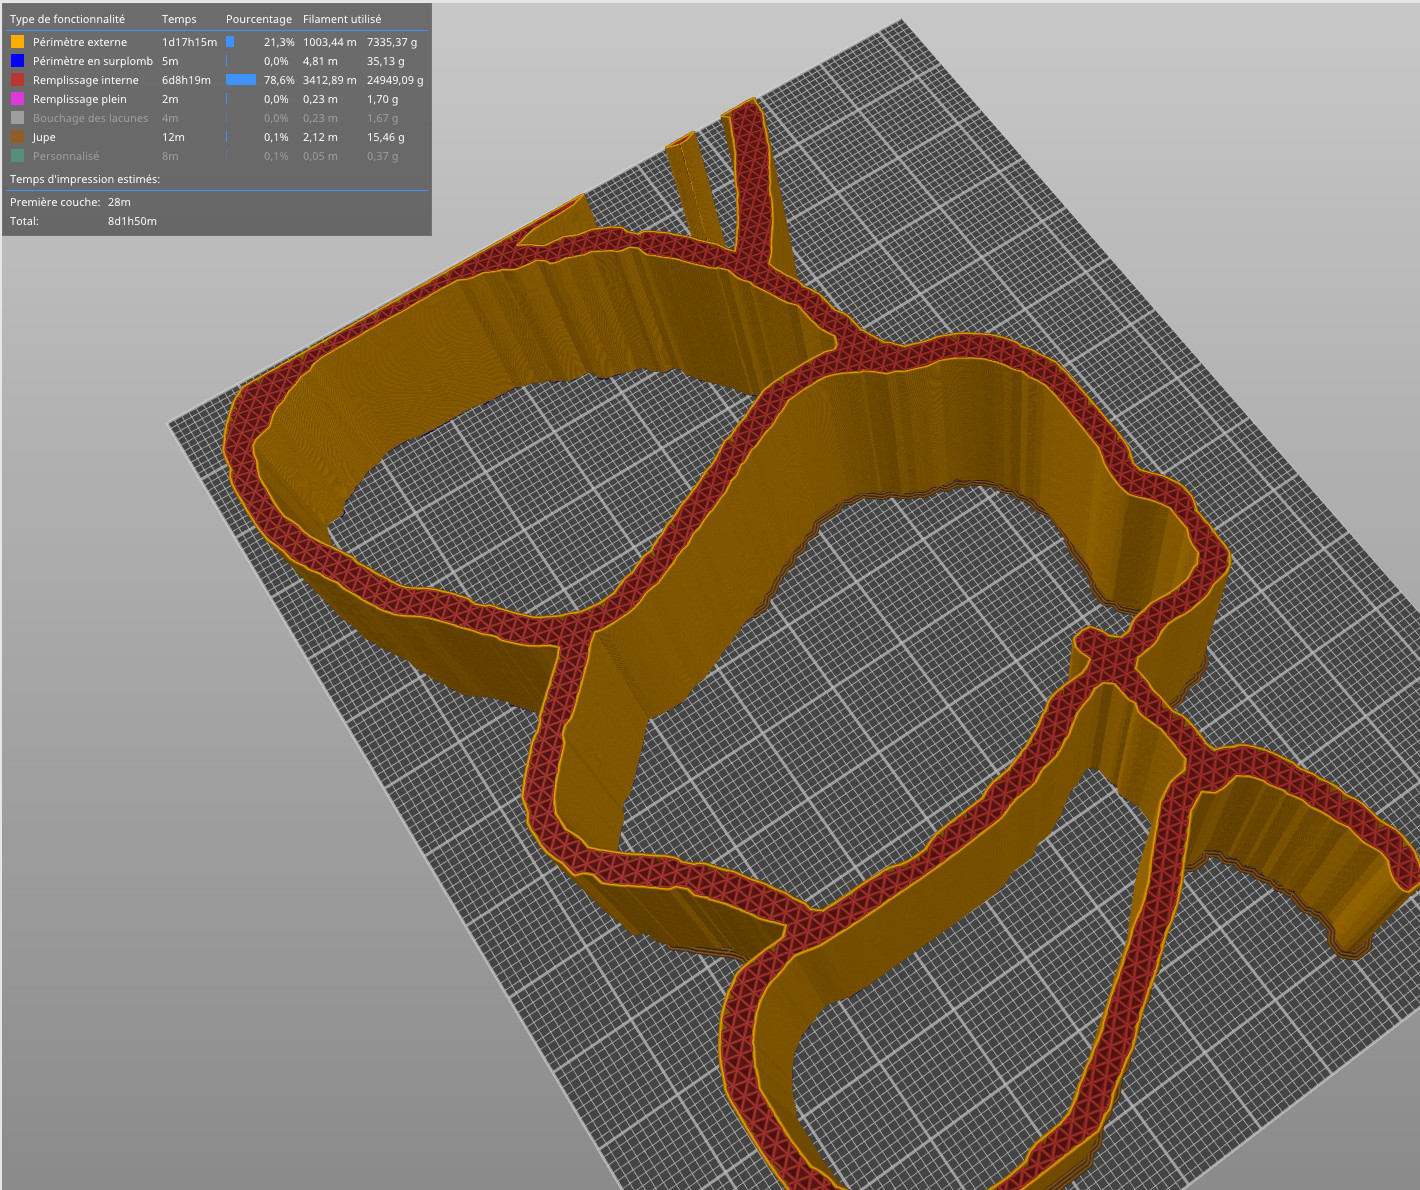
\includegraphics{figures/printing/Slicer.jpg}

}

\caption{\label{fig-gcode}Programmation of the printing process using
the OS SuperSlicer software}

}

\end{minipage}%
%
\begin{minipage}[t]{0.05\linewidth}

{\centering 

~

}

\end{minipage}%
%
\begin{minipage}[t]{0.55\linewidth}

{\centering 

\begin{longtable}[]{@{}ll@{}}
\toprule()
Main parameters & Value \\
\midrule()
\endhead
Material & PET recycled \\
Bed temperature & 84 °C \\
Extrusion factor & 1.32 \\
Nozzle temperature & 264 °C \\
Number of perimeters & 2 \\
Top solid layers & 2 \\
Bottom solid layers & 2 \\
Fill density & 30\% \\
Travel speed & 20 mm/S \\
Nozzle Diameter & 1.75 mm \\
Support & No \\
\bottomrule()
\end{longtable}

}

\end{minipage}%

\end{figure}

\hypertarget{step-8-post-processing}{%
\subsection{Step 8 : Post-processing}\label{step-8-post-processing}}

Post-processing relies on the treatment of the injected and/or printed
part. Regarding the injection part, the post-processing refers to the
surface treatment of the injected part

\begin{figure}[H]

{\centering 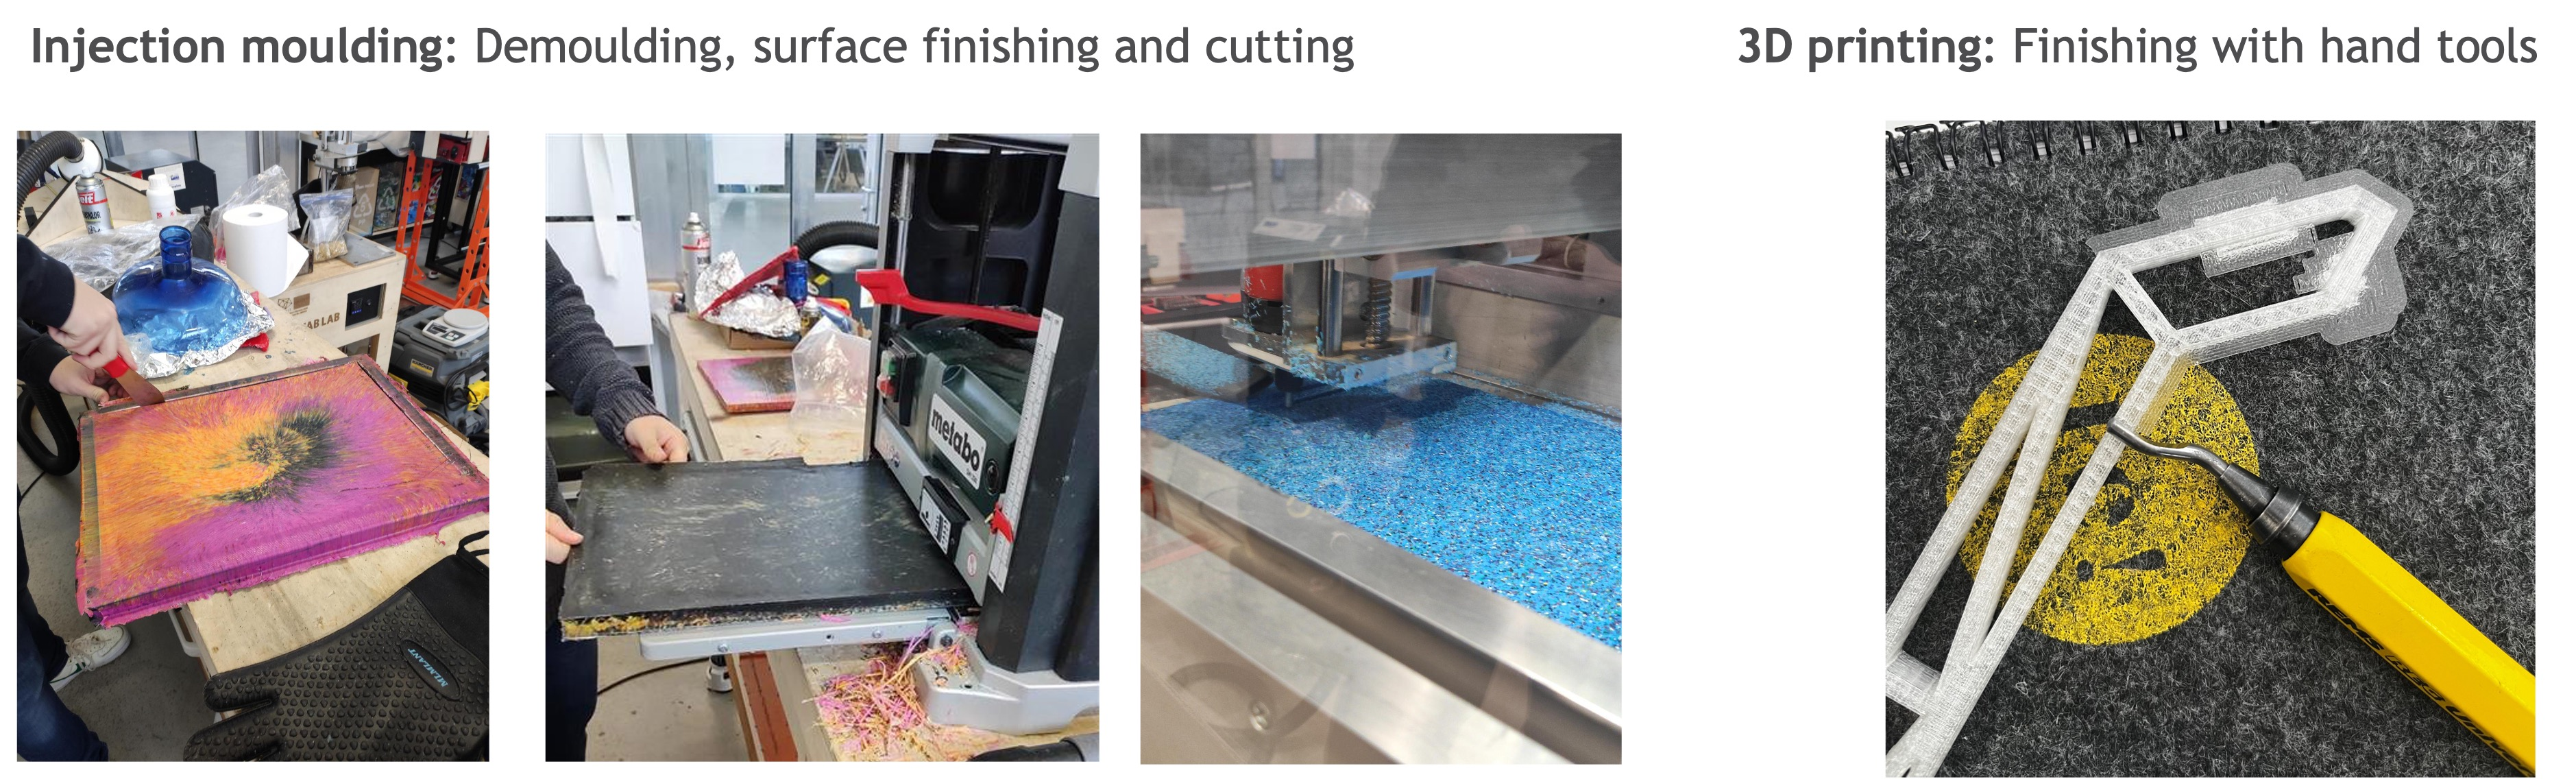
\includegraphics{figures/post-processing.jpg}

}

\caption{Post-processing activities for the injection molding and 3D
printing processes}

\end{figure}

On the other hand, post-processing on the printing part is related to
the removal of excess backing material and the support material used.
These two activities are made manually.

\hypertarget{step-9-implementation-examples}{%
\subsection{Step 9: Implementation
Examples}\label{step-9-implementation-examples}}

The different examples of implementation of the use case are presented
in the following sections. Each example aims to tackle step by step the
complexity of the implementation of the DIT process at a TRL6 level. We
specified in each example the step of the DIT process that aims to test.

\hypertarget{personalization-of-existing-furniture}{%
\subsubsection{Personalization of existing
furniture}\label{personalization-of-existing-furniture}}

This first experimentation aimed to prove the design of a customized
product. Based on the printability tests, the initial model was
developed using the CAD software Onshape to validate the technical
printability of PLA virgin assets. Using the case of a personalization
of a commercial furniture-arranging tool as displayed in
Figure~\ref{fig-demo1}, several printed parts were manufactured to
evaluate the technical pertinence of the results as part of existing
furniture.

\begin{figure}[H]

{\centering 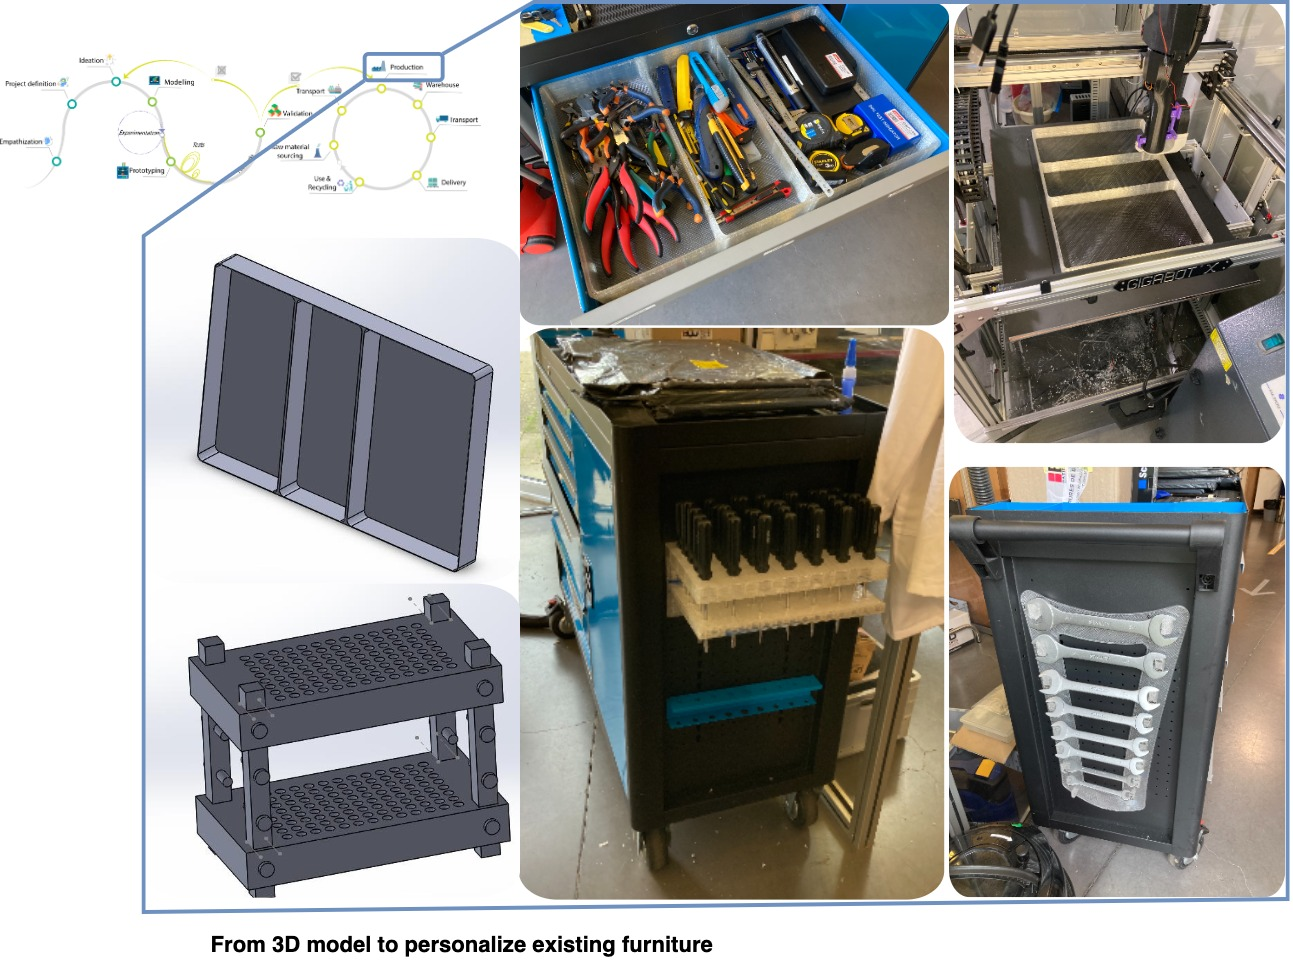
\includegraphics[width=0.8\textwidth,height=\textheight]{figures/Demo-01.jpg}

}

\caption{\label{fig-demo1}Personalizing a existing furniture}

\end{figure}

In this case, only the 3D printer Gigabot was used to validate the
robustness and the quality of the printed part.

\hypertarget{refurbishing-of-the-an-old-furniture}{%
\subsubsection{Refurbishing of the an old
furniture}\label{refurbishing-of-the-an-old-furniture}}

In this case, the experimentation was a step further. The main idea was
to refurbish an old wood workbench, connecting the tools of INEDIT.
Therefore, the idea was to use the scanner and the sketch features of
the DesignTogether tool developed by the colleges of INEDIT. Based on
those inputs, the manufacturing tools at the Green fablab including the
3D printing were mobilized.

\begin{figure}[H]

{\centering 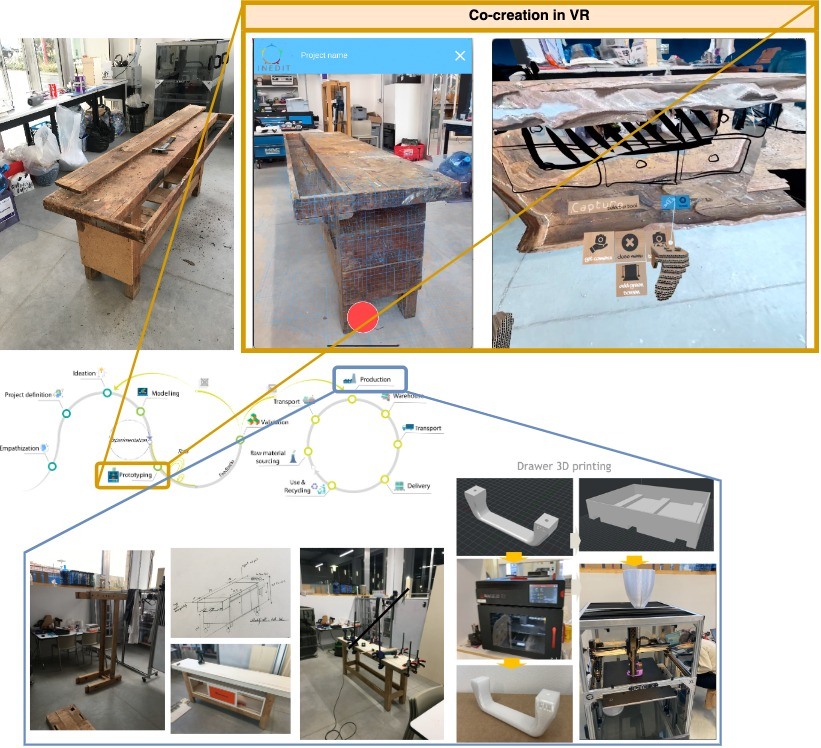
\includegraphics[width=5.20833in,height=\textheight]{figures/Demo-02.jpg}

}

\caption{\label{fig-workbench}Refurbishing an old wood workbench using
the INEDIT technologies}

\end{figure}

Figure~\ref{fig-workbench} presents the processes entailed in the
experimentation. First, once the workbench was dismantled, it was
scanned using an Ipad Pro considering the technical characteristics
needed for the application. Then, the model was uploaded in the
DesignTogether application in order to brainstorm ideas of features that
are required to consider for the refurbishing. This was in input in the
co-creation aspect of the process.

\begin{figure}

\begin{minipage}[t]{0.35\linewidth}

{\centering 

\raisebox{-\height}{

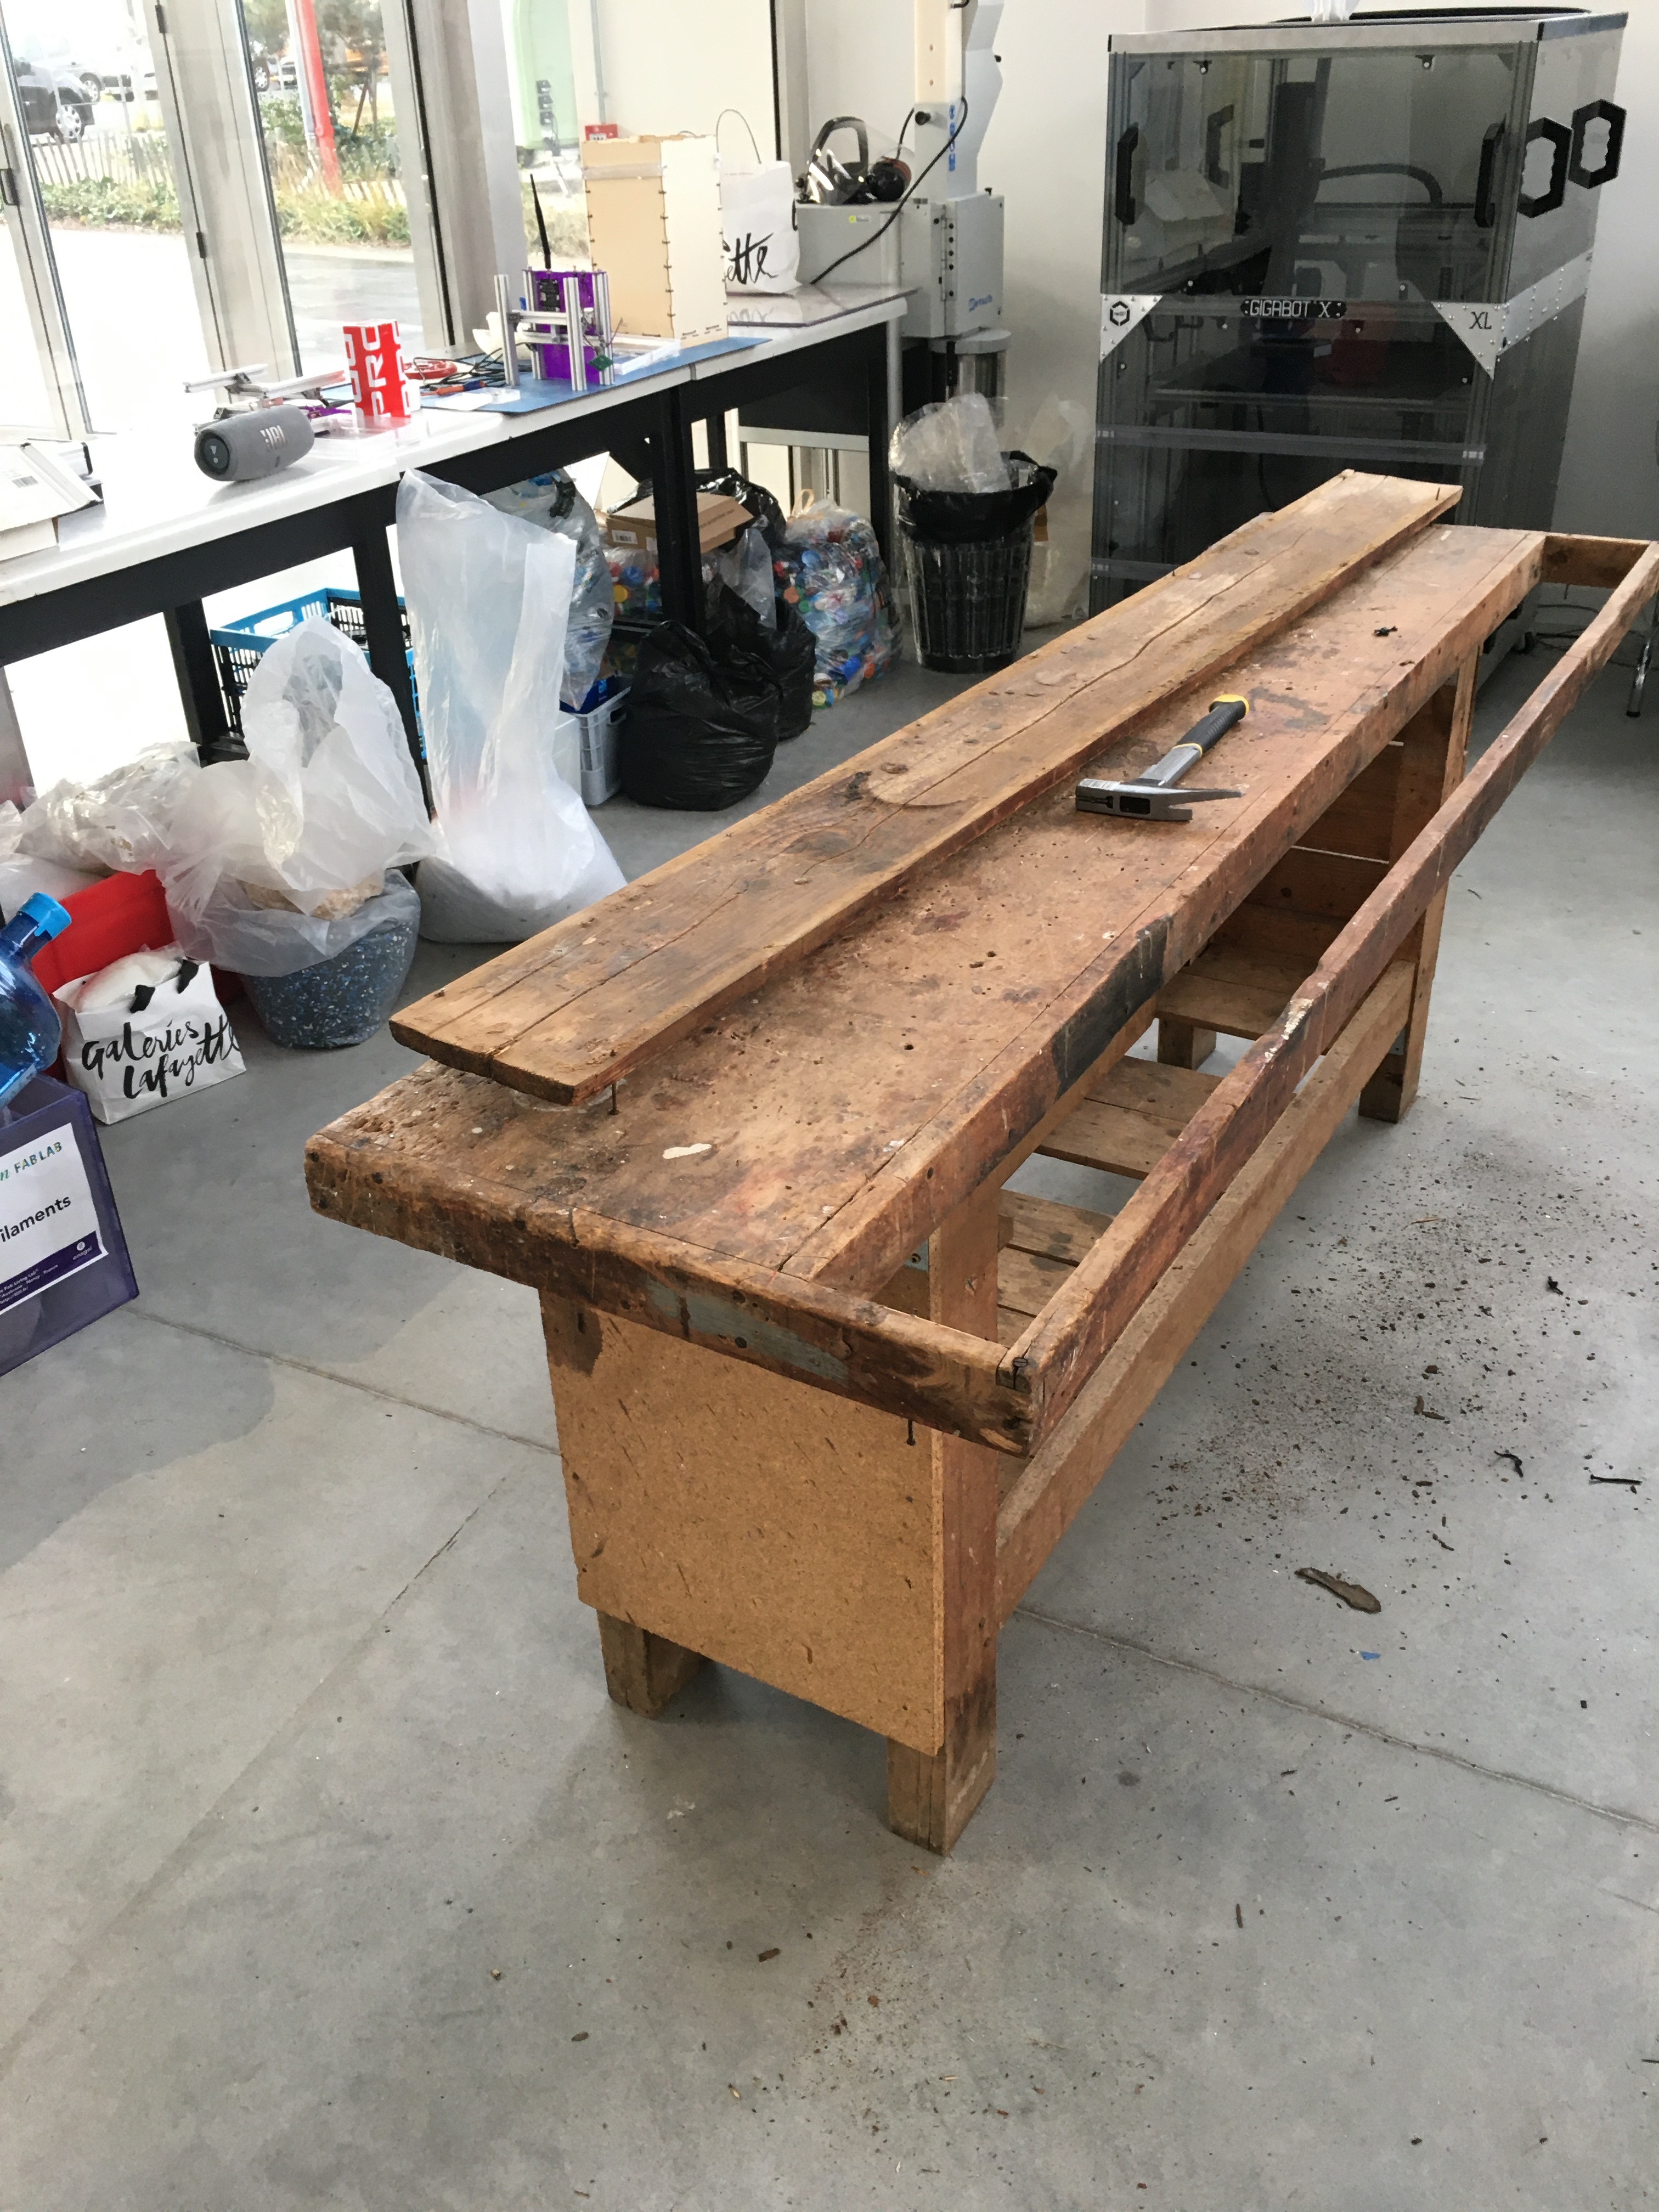
\includegraphics{figures/demos/workbench/Initial.jpg}

}

}

\subcaption{\label{fig-demo2.1}Initial recovered workbench}
\end{minipage}%
%
\begin{minipage}[t]{0.05\linewidth}

{\centering 

~

}

\end{minipage}%
%
\begin{minipage}[t]{0.60\linewidth}

{\centering 

\raisebox{-\height}{

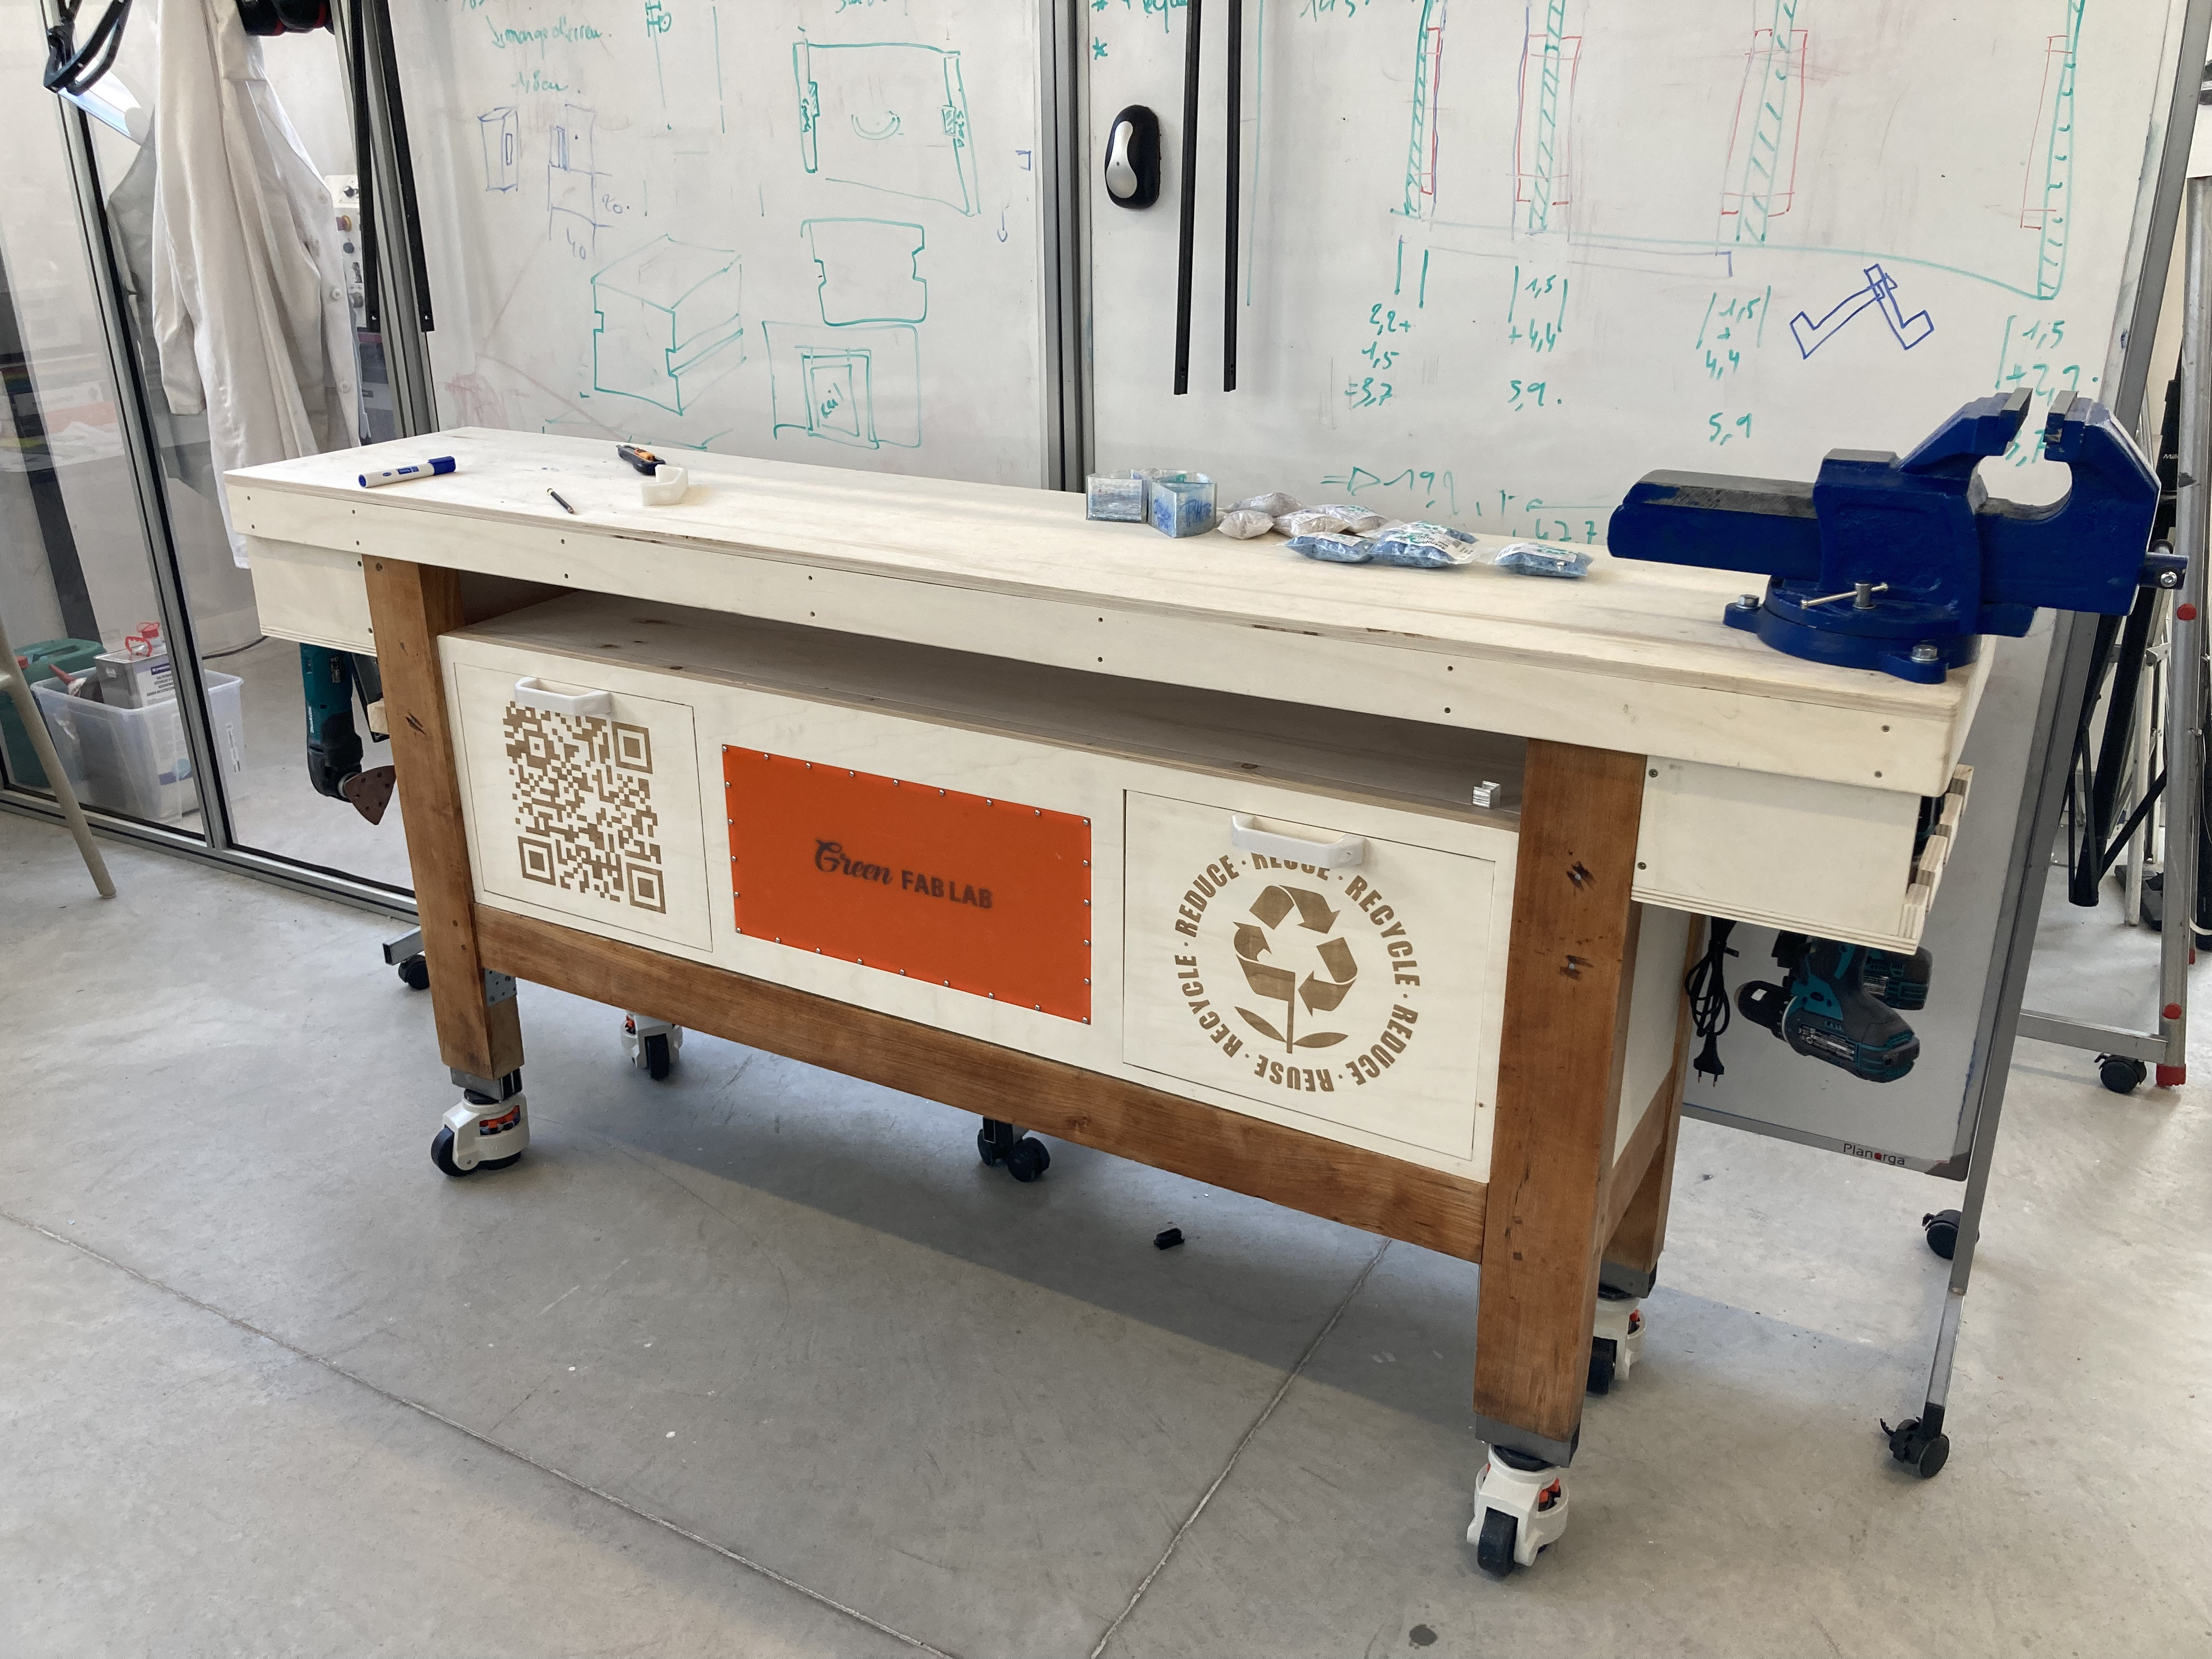
\includegraphics{figures/demos/workbench/Final.jpeg}

}

}

\subcaption{\label{fig-demo2.2}Refurbished workbench}
\end{minipage}%

\caption{\label{fig-demo2}Experimentation on refurbishing a wood
workbench model}

\end{figure}

Afterwards, the model enables a first materialization of the proposition
that could be made. So, the different manual task started in function

\hypertarget{connecting-the-recycling-part-and-the-smartification}{%
\subsubsection{Connecting the Recycling part and the
Smartification}\label{connecting-the-recycling-part-and-the-smartification}}

In this experimentation, the idea was to connect the smartification
process developed by the Uninova partners with the capabilities of our
use case manufacturing. The purpose was to build a piece of furniture to
test the integration of the plastic and smartification technologies. In
this case, Figure~\ref{fig-uninova} illustrates the manufacturing of a
recycled plastic bar specifically made to be part of the entire
furniture.

\begin{figure}[H]

{\centering 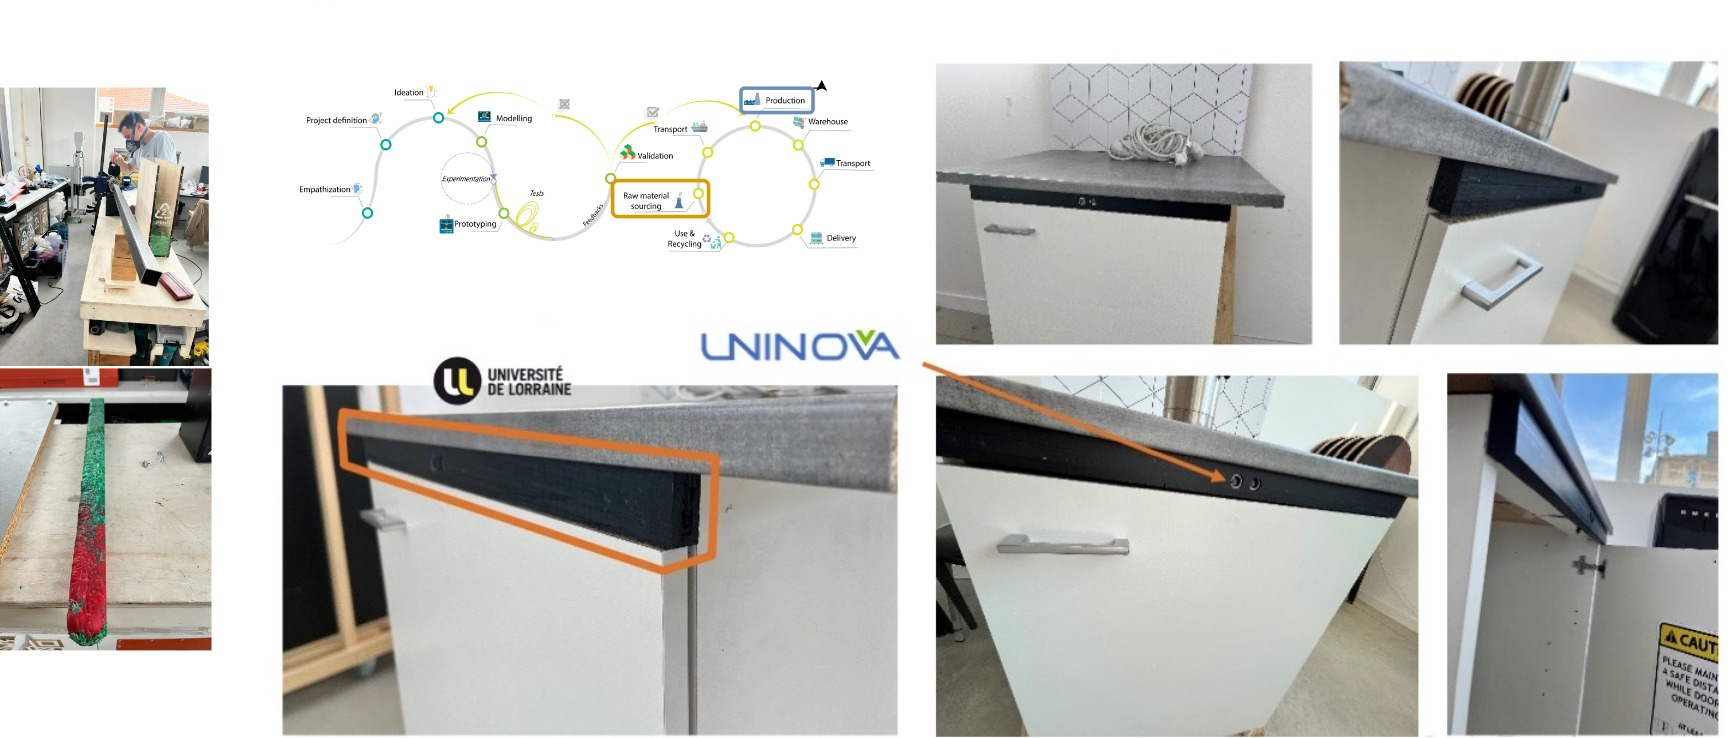
\includegraphics[width=0.9\textwidth,height=\textheight]{figures/demos/Uninova/Uninova-01.jpg}

}

\caption{\label{fig-uninova}Fabrication of a prototype kitchen at the
ICE-IAMOT Conference at Nancy June 2022}

\end{figure}

Therefore, as a part of the ICE-IAMOT conference demonstrator that took
place on June 2022 at Nancy, We have built the complete wood structure
of a kitchen furniture as presented in the Figure~\ref{fig-uninova-00}.
The colleges of Uninova installed the electrical components in order to
adjust the kitchen to the smart options. Here, the recycled plastic bar
was used as sensor protection and masking of the sensor needed in the
electrical mounting. Moreover, the value of the recycled material added
a personalisation finishing of the final prototype.

\begin{figure}[H]

{\centering 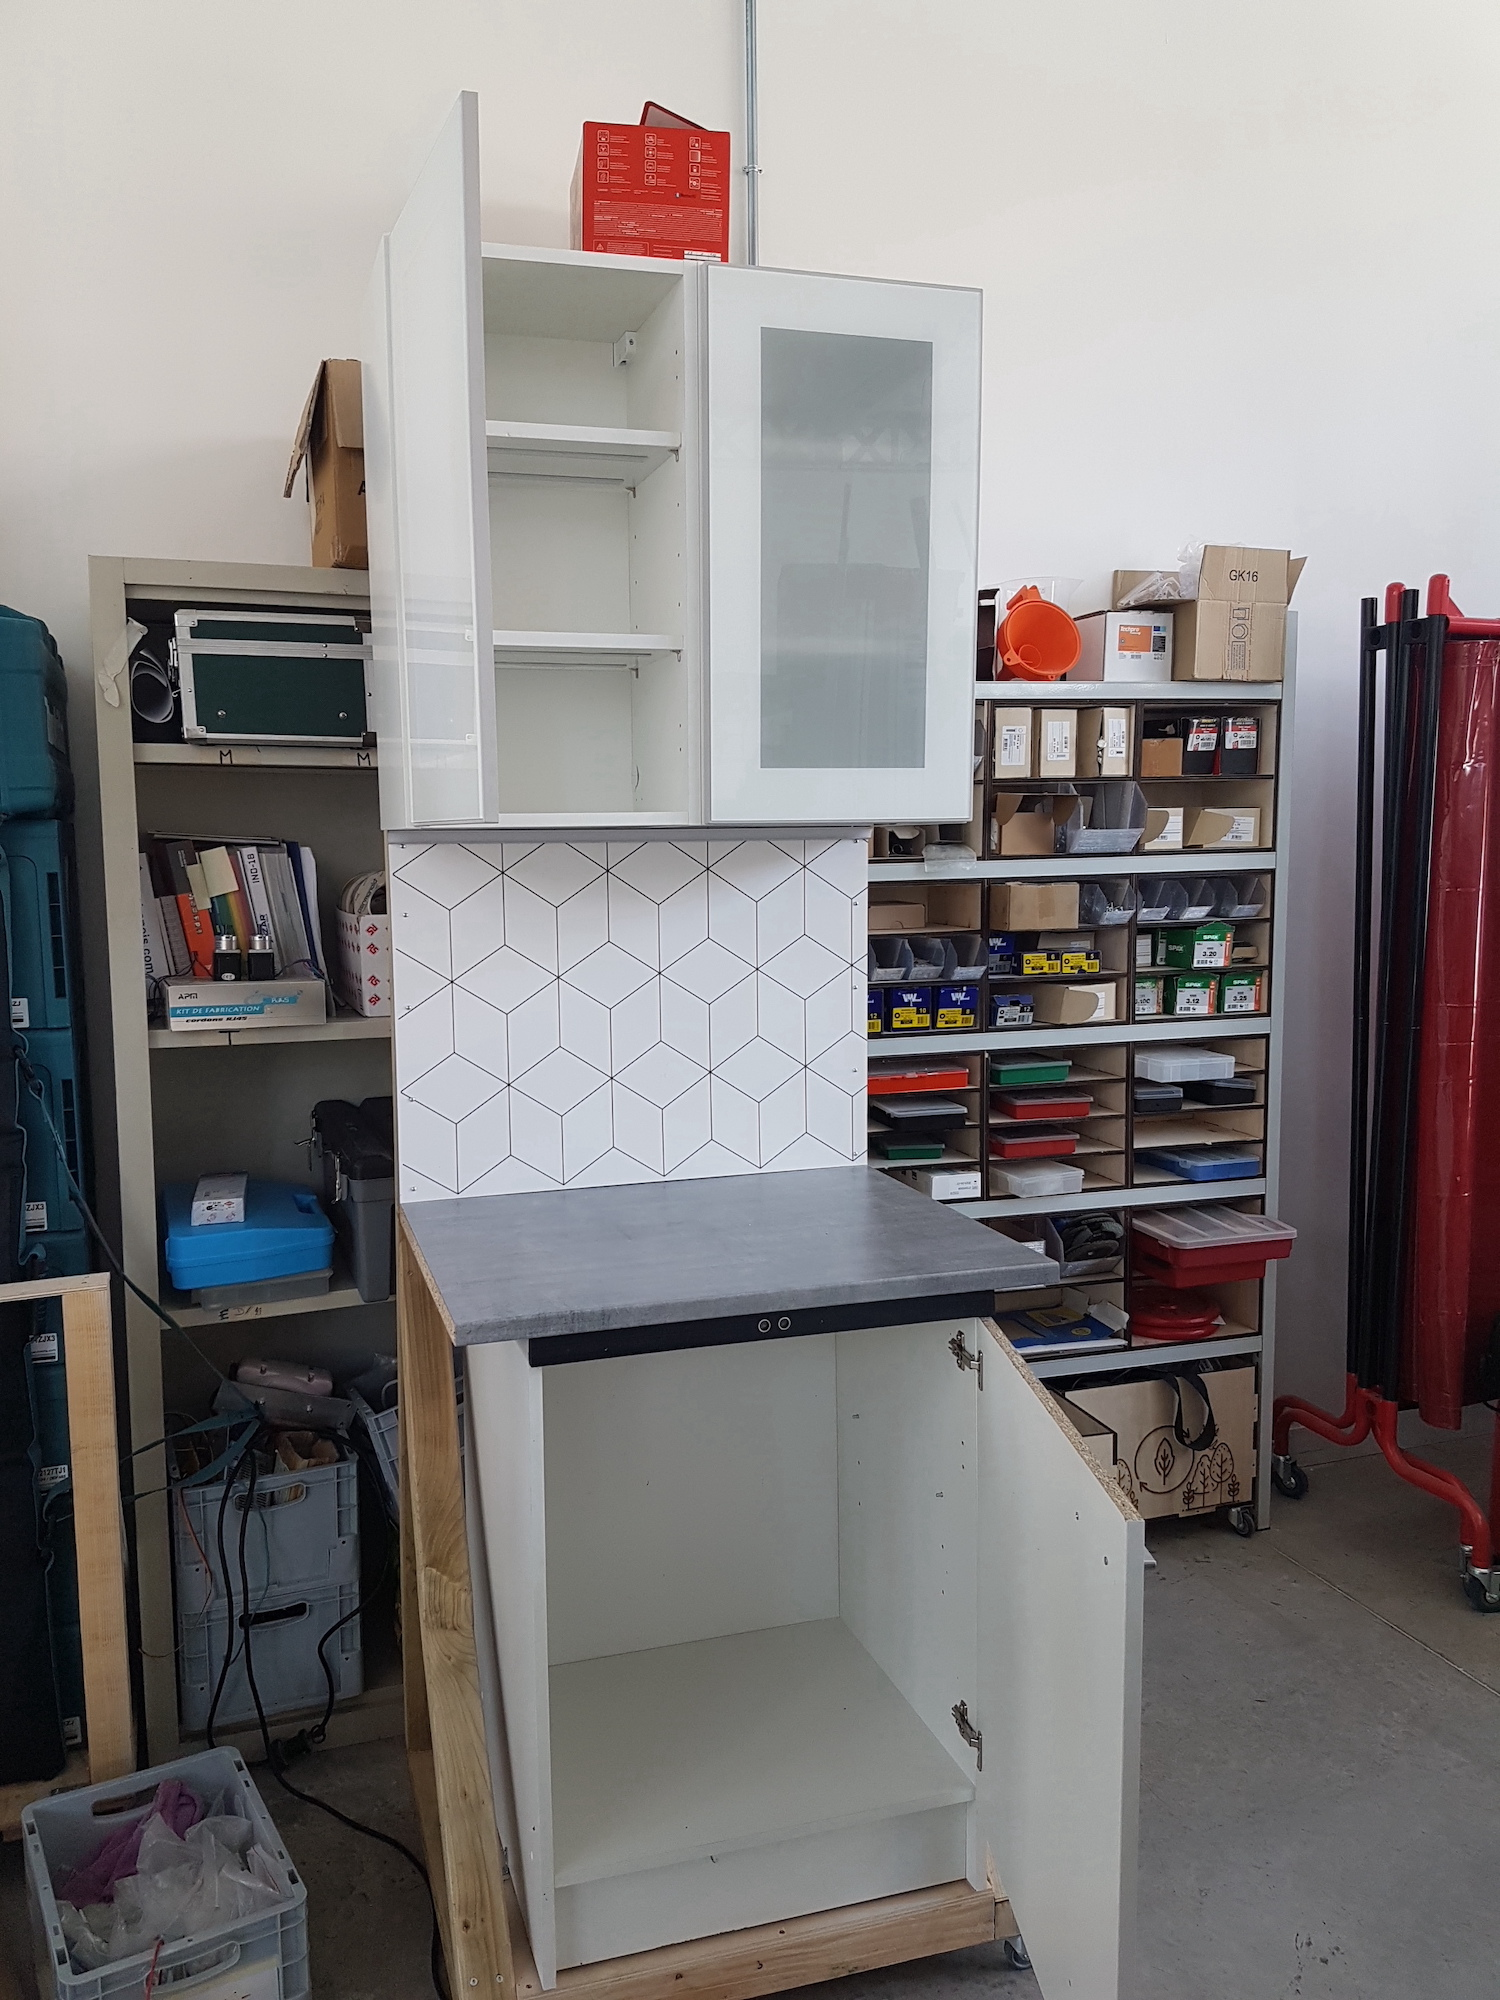
\includegraphics[width=3.125in,height=\textheight]{figures/demos/Uninova/uninova-00.jpg}

}

\caption{\label{fig-uninova-00}Smartification of a kitchen}

\end{figure}

\hypertarget{collaborative-desk-and-bookshelf}{%
\subsubsection{Collaborative Desk and
Bookshelf}\label{collaborative-desk-and-bookshelf}}

At the INEDIT consortium, it was decided to build a collaborative desk
and a bookshelf. The challenge in this experimentation was to connect
all the different competences that are present in the different use
cases. Regarding our use case, we supported the creation of the
prototype of this desk in a reduced scale using recycled filament.
Additionally, it was also the opportunity to make recycled production
from printing and injection processes for the customization pieces.

Firstly, Figure~\ref{fig-desk-00} illustrates several attempts made
using the DesignTogether tool for ideas of personalization of the
furniture. A workshop with 20 students of the National National School
of Industrial Systems Engineering (ENSGSI) was organized to create
several ideas on the same object.

\begin{figure}[H]

{\centering 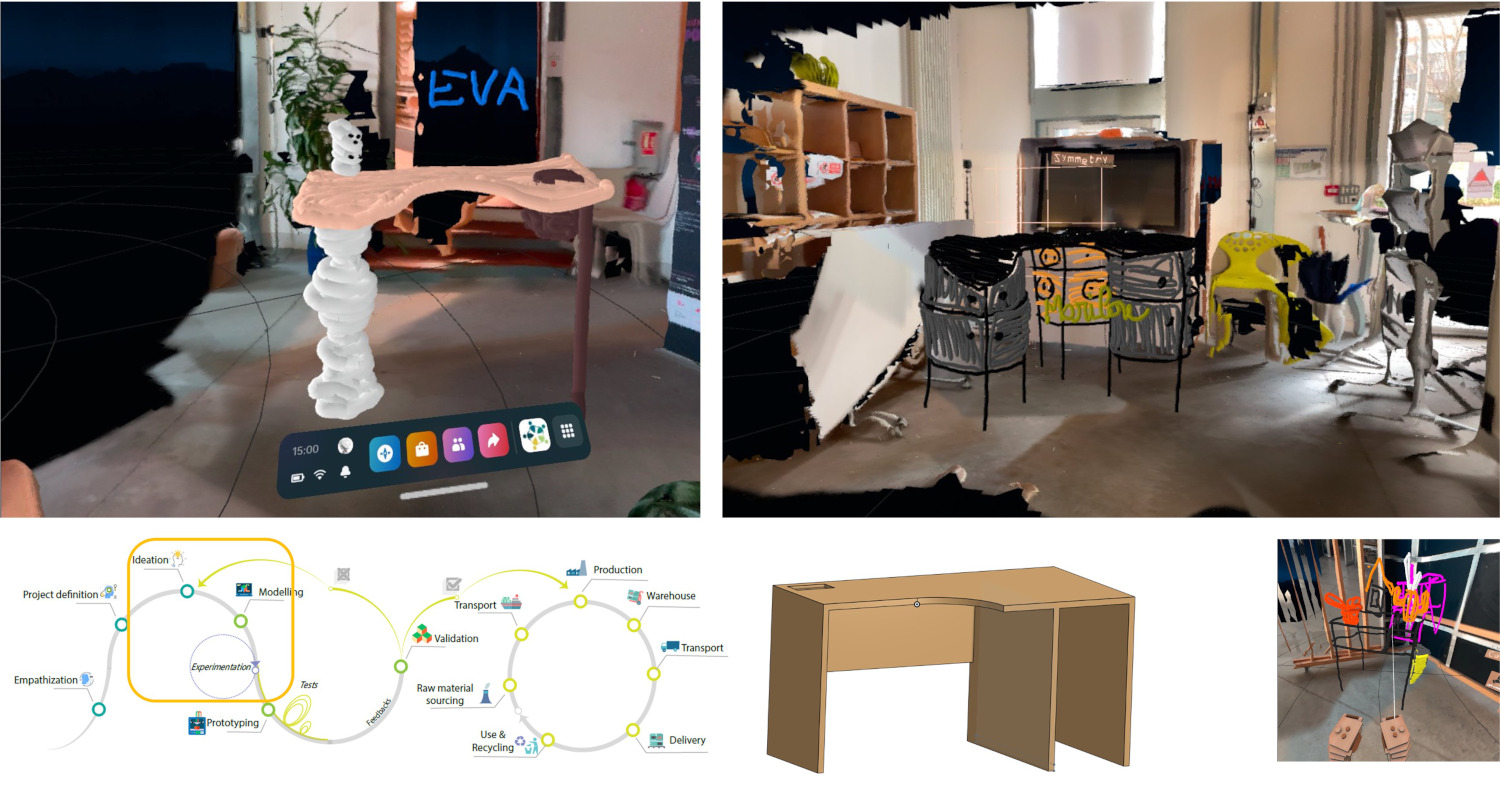
\includegraphics[width=0.95\textwidth,height=\textheight]{figures/demos/desk/desk-00.jpg}

}

\caption{\label{fig-desk-00}Co-creation stage on the personalization for
the}

\end{figure}

Once the ideation phase was made, a second step was focused on the
manufacturing of a small prototype of the desk using plastic assets as
presented in figure Figure~\ref{fig-desk-01}. This made it possible to
define the components that were manufactured at real scale.

\begin{figure}[H]

{\centering 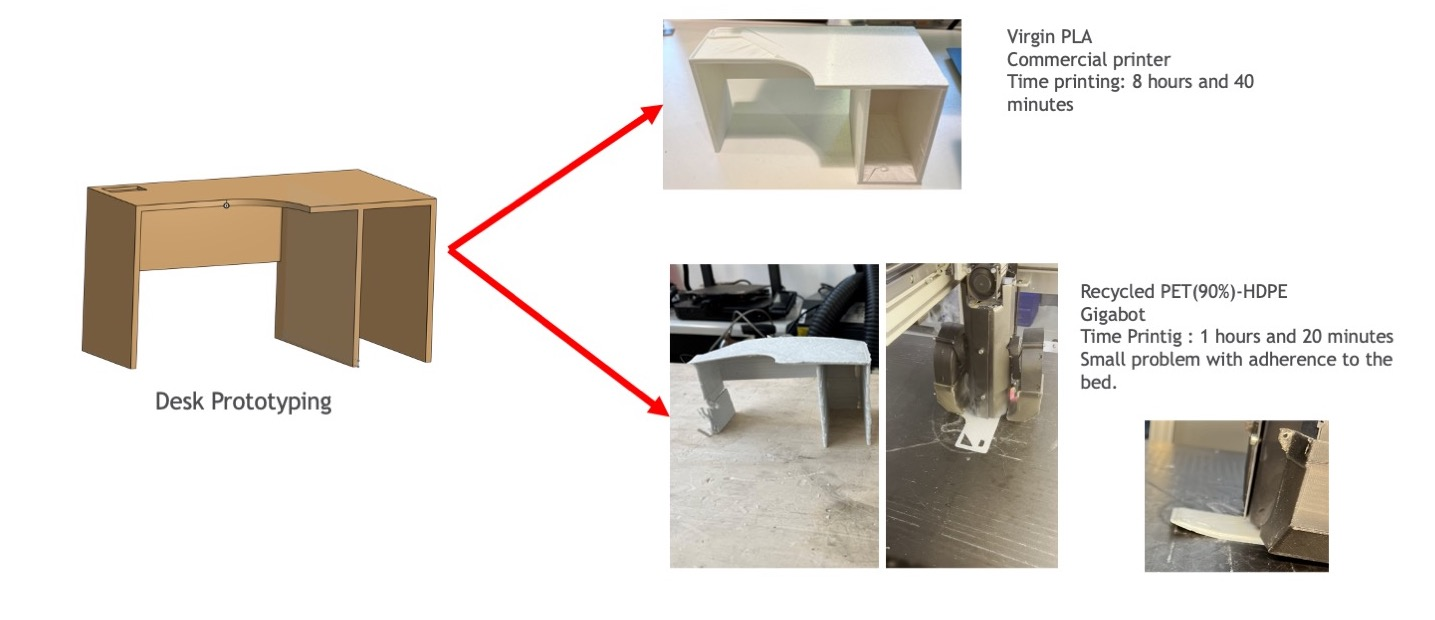
\includegraphics[width=0.95\textwidth,height=\textheight]{figures/demos/desk/desk-01.jpg}

}

\caption{\label{fig-desk-01}Prototype of the desk}

\end{figure}

The prototype enabled to identify three main customization object,
namely 1) PC monitor support, 2) an adjustable folder separation and 3)
the drawer handler. as displayed in the Figure~\ref{fig-desk-01}. The PC
monitor support was built entirely using the manual injection molding.
The drawer handler was completely 3D printed. Finally, the adjustable
folder was a combination of injection and 3D printed processes

\begin{figure}[H]

{\centering 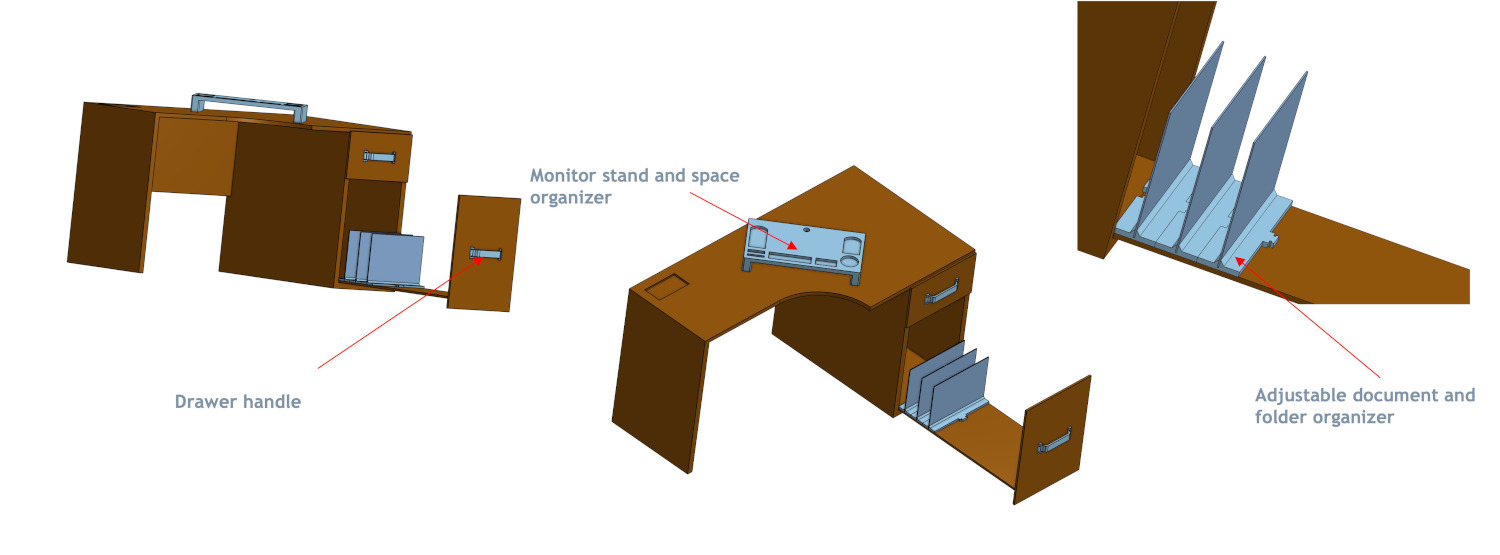
\includegraphics{figures/demos/desk/desk-02.jpg}

}

\caption{\label{fig-desk-01}3D model of the recycled pieces to be made}

\end{figure}

\begin{figure}[H]

{\centering 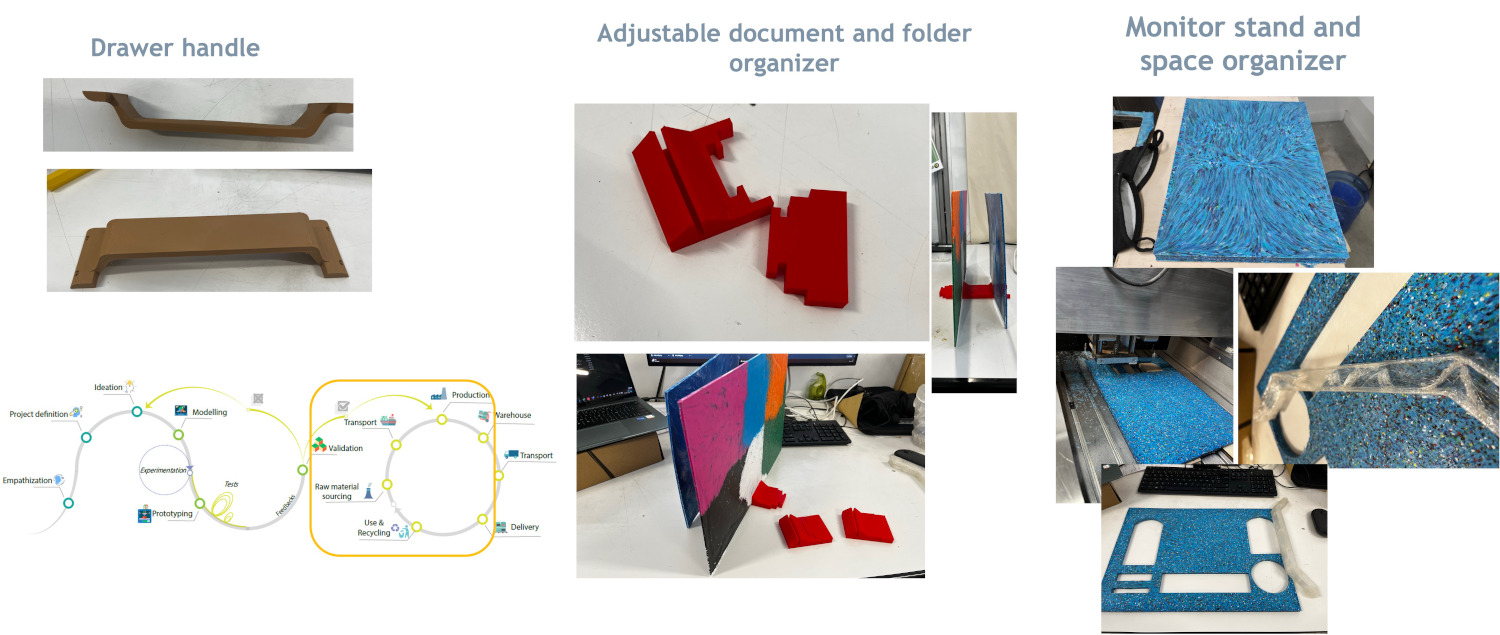
\includegraphics{figures/demos/desk/desk-03.jpg}

}

\caption{\label{fig-uninova-01}Manufacturing of the recycled parts (PC
support, adjustable folder separation and drawer handler)}

\end{figure}

This experimentation was then confronted with the consortium to obtain
feedback about the possible improvements in the technical level as
presented in the Figure~\ref{fig-desk-final}. But more importantly, to
identify the possible continuum and interaction between the different
technologies and models.

Regarding the bookshelf, we could printed a prototype version of the STL
model that was generated in the co-creation phase of the platform as
displayed in the Figure~\ref{fig-book-1} and Figure~\ref{fig-book-2}.

\begin{figure}

\begin{minipage}[t]{0.60\linewidth}

{\centering 

\raisebox{-\height}{

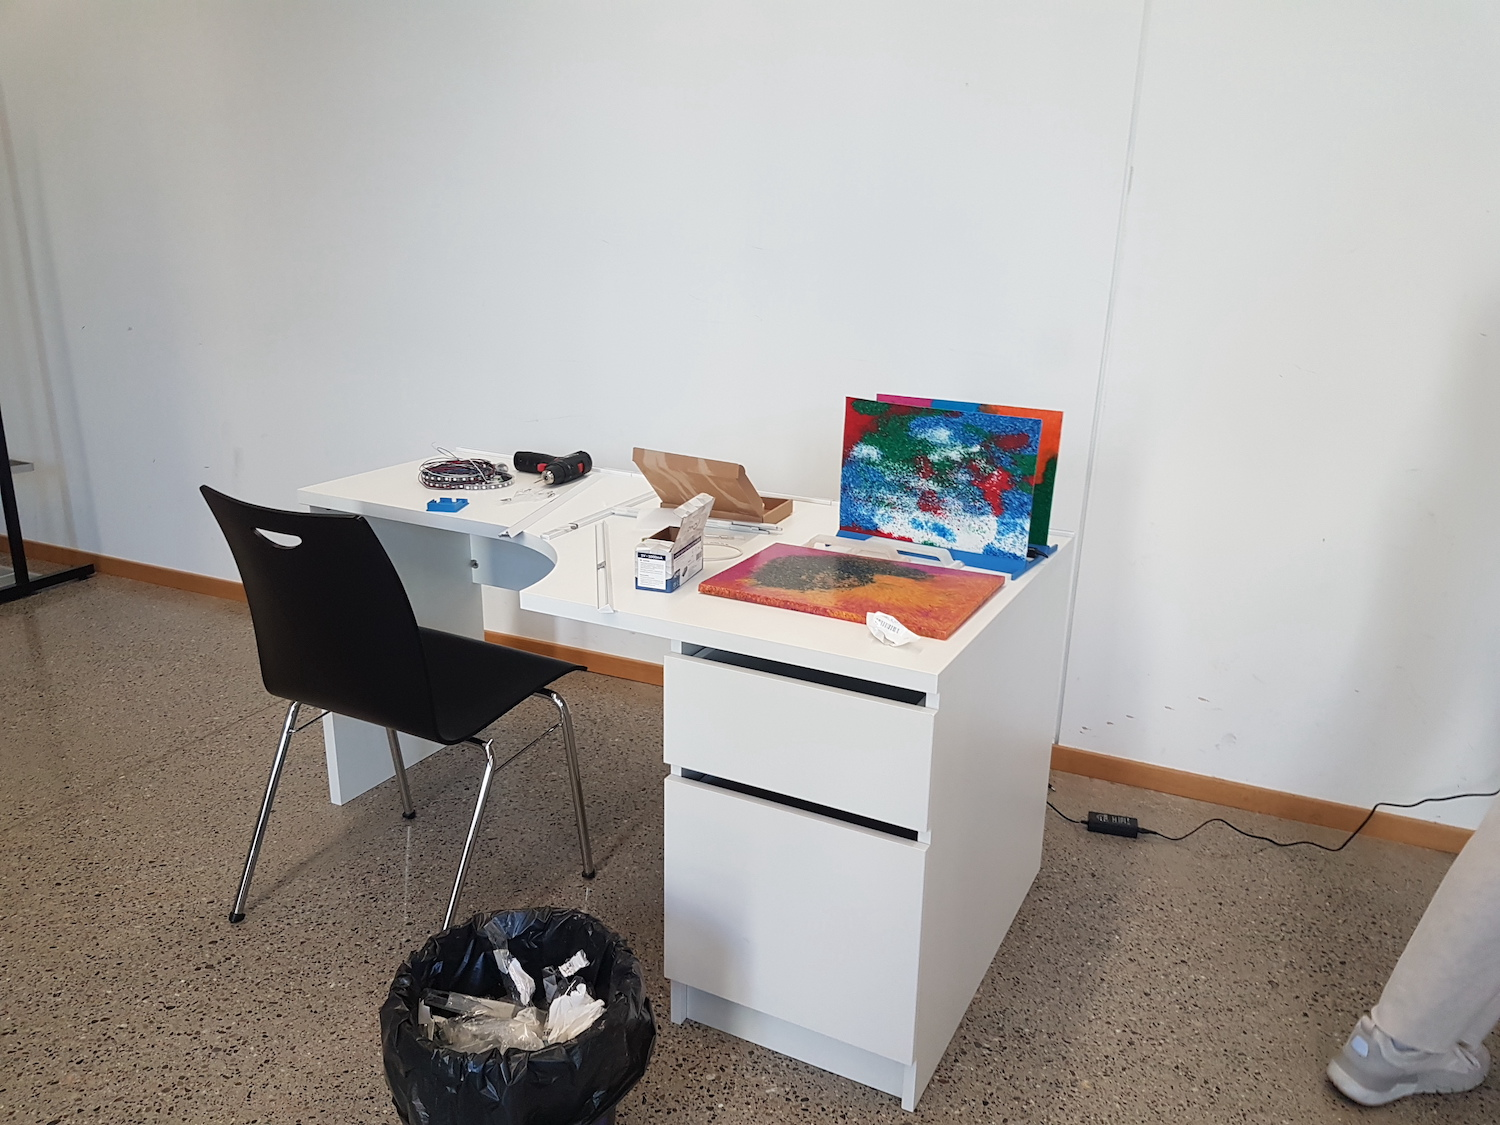
\includegraphics{figures/demos/desk/desk-04.jpg}

}

}

\subcaption{\label{fig-desk-04}Final assembling of the desk}
\end{minipage}%
%
\begin{minipage}[t]{0.05\linewidth}

{\centering 

~

}

\end{minipage}%
%
\begin{minipage}[t]{0.35\linewidth}

{\centering 

\raisebox{-\height}{

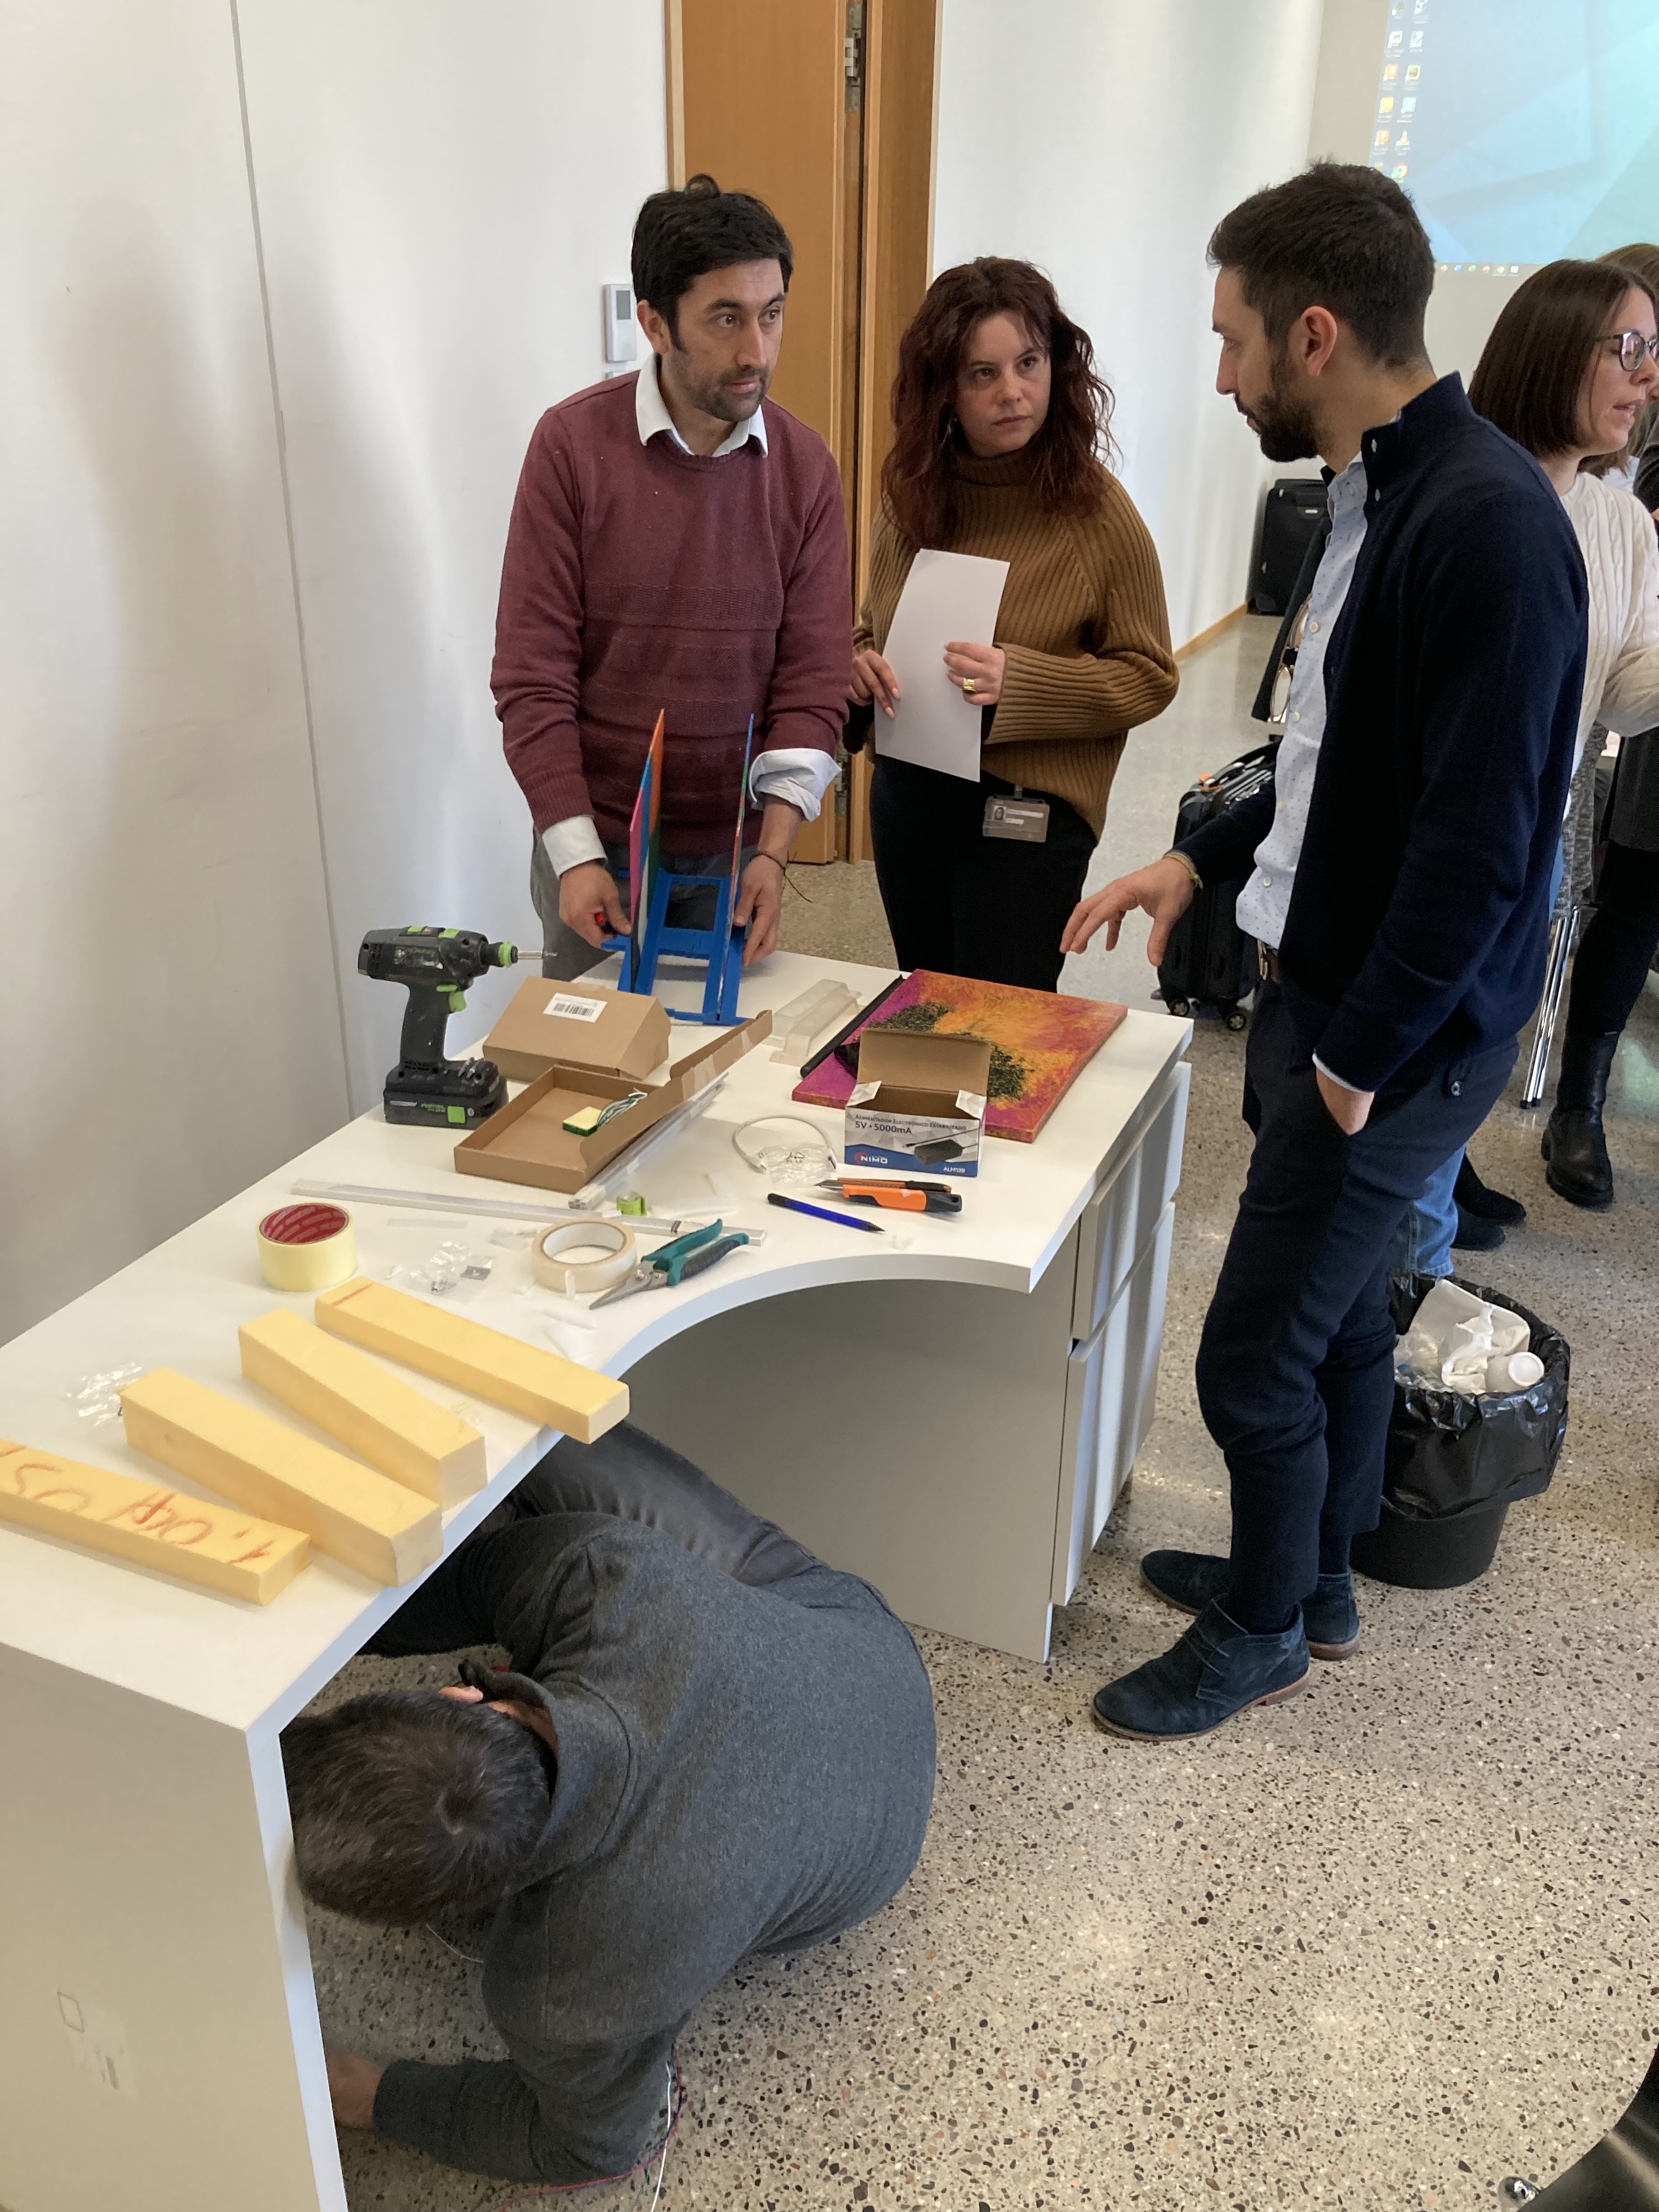
\includegraphics{figures/demos/desk/desk-05.jpg}

}

}

\subcaption{\label{fig-desk-05}Exchange and discussion on the
interaction and possible improvements}
\end{minipage}%

\caption{\label{fig-desk-final}Feedbacks on the improvement of the
recycled printed and injected parts}

\end{figure}

\begin{figure}

\begin{minipage}[t]{0.47\linewidth}

{\centering 

\raisebox{-\height}{

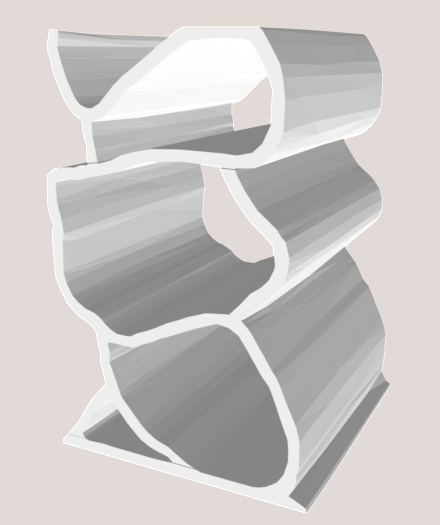
\includegraphics{figures/demos/book/book-stl.png}

}

}

\subcaption{\label{fig-book-1}Bookshelf 3D model}
\end{minipage}%
%
\begin{minipage}[t]{0.10\linewidth}

{\centering 

~

}

\end{minipage}%
%
\begin{minipage}[t]{0.42\linewidth}

{\centering 

\raisebox{-\height}{

\includegraphics{figures/demos/book/book-2.jpg}

}

}

\subcaption{\label{fig-book-2}Printed Bookshelf as a prototype}
\end{minipage}%

\caption{\label{fig-desk-final}Bookshelf demonstration with the STL
model and the 3D printed prototype.}

\end{figure}

\newpage

\hypertarget{local-collaboration-with-the-green-fablab-the-case-of-the-le-spationef-lappaillet}{%
\subsection{Local collaboration with the Green fablab: the case of the
``Le Spationef \&
L'appaillet''}\label{local-collaboration-with-the-green-fablab-the-case-of-the-le-spationef-lappaillet}}

One important element of the INEDIT project is the interaction with
external designers and the local ecosystem. The implementation of the
Green Fablab inside the Octroi ecosystem makes this interaction valuable
and fruitful to better align the expectations of designers and
architects with the possible maturity that the different technologies
can have inside the INEDIT project.

For instance, Figure~\ref{fig-eddy} displays a collaboration with a
local micro-architecture collective of called
\href{https://www.octroi-nancy.fr/2020/10/29/collectif-hobo/}{Le
Spationef}, where the main objet was to make a prototype of a concept of
furniture.

\begin{figure}[H]

{\centering \includegraphics[width=0.9\textwidth,height=\textheight]{figures/demos/apa/eddy.jpg}

}

\caption{\label{fig-eddy}Sketch models designed by the local actor Le
Spationef}

\end{figure}

The prototype of the roof was made using the desktop plastic machine
tested in the Green Fablab. THe interaction with this local architect
enable us to see the pertinence of have the plastic recycling
capabilities for sheet plastic part. They pointed out that this type of
prototyping aspects can be useful in particular furniture where the wood
furniture is adequate.

Based on these insgths, in another example, we made an experimentation
project with the local association of designers called
\textbf{L'A.Paillette}\footnote{See the communication page at
  https://www.facebook.com/L.A.Paillettes/}. The purpose was to not only
create a prototype part but a fonctional part that can be used by the
Octroi community. Thus, the project was to design and build 3 mobile
modules and movable for a kitchen. These modules will allow heating
equipment, preparation equipment and cleaning equipment to be placed and
moved.

\begin{figure}[H]

{\centering \includegraphics[width=0.9\textwidth,height=\textheight]{figures/demos/apa/Modeles-Furniture-00.jpg}

}

\caption{\label{fig-apa-00}Sketch models designed by the local actor
L'A.Paillette}

\end{figure}

The first proposition of the models are presented in the
Figure~\ref{fig-apa-00}.

\begin{figure}[H]

{\centering \includegraphics[width=0.9\textwidth,height=\textheight]{figures/demos/apa/iteration.jpg}

}

\caption{\label{fig-iteration}Iteration and re-design of the proposed
recycled parts}

\end{figure}

Several iterations were needed in order to transform the initial
requirement into possible manufactured pieces given the possibilities of
the technology presented in our use case as displayed in
Figure~\ref{fig-iteration}. Based on a prototype and a test by use, we
could identify certain failures in the proposed part. Therefore, the
failure was improved and corrected involving the designers of the
l'A.Paillette.

\begin{figure}

\begin{minipage}[t]{\linewidth}

{\centering 

\raisebox{-\height}{

\includegraphics[width=4.16667in,height=\textheight]{figures/demos/apa/final-01.jpg}

}

}

\subcaption{\label{fig-apa-00}Final overview of the kitchen}
\end{minipage}%
\newline
\begin{minipage}[t]{\linewidth}

{\centering 

\raisebox{-\height}{

\includegraphics[width=4.16667in,height=\textheight]{figures/demos/apa/final.jpg}

}

}

\subcaption{\label{fig-apa-00}Recycled plastic parts implemented}
\end{minipage}%

\caption{\label{fig-apa-final}Final furniture made in collaboration with
the local designers at Octroi.}

\end{figure}

The production consisted on 3 sheets. After several attempts, a version
of recycled wheets, pins were decided to fabricate. This final model was
fabricated using 400g per sheet, 96 plastic pin joints (20g per pin),
having a total recycled plastic used about 3,1 kg approx. (around 800
bottle taps). The final furniture made is presented in the
Figure~\ref{fig-apa-final}.

\newpage

Finally, given the local establishment of the the team of the Green
Fablab demonstrator at the Octroi ecosystem, the local mayor's office of
Nancy organized a ``Zero Waste Market'' on December 2022.
Figure~\ref{fig-zero} illustrates the participation of the Green Fablab
team, an it was an excellent opportunity to make a communication and
dissemination with general public on the INEDIT projet and the
importance of plastic recycling issues

\begin{figure}[H]

{\centering \includegraphics[width=5.20833in,height=\textheight]{figures/demos/apa/zero-dechets.jpg}

}

\caption{\label{fig-zero}Participation of Green Fablab to the Zero Waste
Market organized by the mayor city at December 2022}

\end{figure}

\newpage

\hypertarget{conclusions}{%
\section{Conclusions}\label{conclusions}}

In this report, we described the research and development work developed
in the task Task 6.4. Mainly, the open manufacturing demonstration
facility of ``3D printing of recycled plastic demonstrator' (also known
as `Green Fablab') developed in the INEDIT project. The main goal was
the validation of the logistical and technical feasibility of recycled
assets to be used in the Do‐It‐Together (DIT) approach.

This rapport showed:

\begin{itemize}
\tightlist
\item
  a conceptual and a technical implementation of the distributed
  recycling via additive manufacturing (DRAM) approach for the INEDIT.
  This conceptual approach is a major scientific output of the INEDIT
  project.
\item
  A step-by-step process was shown to illustrate the materialization of
  the 3D printing of plastic recycling demonstrator.
\item
  Several implementation examples were presented in order to validate
  technical advancement, but more importantly, to highlith the
  territorial impact that this type of initiatives can have.
\end{itemize}

The work developed in this task explores new and responsible tools that
can act as drivers in a social manufacturing platform like INEDIT. The
results of this example can create new business models and markets in
the furniture sector and also establish new technology for the flexible
manufacturing of customized furniture.

A large number of products can already be manufactured with AM, which
affects the geographical spread and density of global value chains
(\protect\hyperlink{ref-Laplume2016}{Laplume et al., 2016}). It is
expected that the reach of AM printable products will be much greater in
the future, as the production of multi-material and built-in
functionalities (e.g.~electronics) will be possible to a large extent.

Nevertheless, more examples are needed in the DRAM for education,
prototyping and semi-industrial purposes. There are complexities in the
recycling aspect given the variability and the plastic waste
contamination. However, given that the AM technology makes it possible
to reduce market entry barriers, reduce capital requirements, major
research and development experimentation can be made to achieve an
efficient minimum scale of production to promote distributed, flexible
forms of production (\protect\hyperlink{ref-Despeisse2016}{Despeisse et
al., 2017}).\\
Taking this into account, the DRAM system presents significant potential
in the future as an option to address the environmental problems linked
to plastic waste, where increased quantity and use of 3D printing allows
more recycled plastic assets to be produced and utilized.

Also, the stages of distributed model factories and decentralized
production types are emerging ranging from distributed capabilities to
cloud production. Thus, the need of transport will be much more
carefully because the fact that AM will enable decentralization of
production to localities near customers or in the most extreme
distributed scenario at the customer's premises
(\protect\hyperlink{ref-BonninRoca2019}{Bonnín Roca et al., 2019};
\protect\hyperlink{ref-Petersen2017a}{Petersen and Pearce, 2017};
\protect\hyperlink{ref-Wittbrodt2013}{Wittbrodt et al., 2013}). This is
a relevant future path for the European union.

\newpage

\hypertarget{bibliography}{%
\section{Bibliography}\label{bibliography}}

\hypertarget{refs}{}
\begin{CSLReferences}{1}{0}
\leavevmode\vadjust pre{\hypertarget{ref-Bano2020}{}}%
Bano, A., Ud Din, I., Al-Huqail, A.A., 2020. {AIoT-Based Smart Bin} for
{Real-Time Monitoring} and {Management} of {Solid Waste}. Scientific
Programming 2020. \url{https://doi.org/10.1155/2020/6613263}

\leavevmode\vadjust pre{\hypertarget{ref-Beltagui2020}{}}%
Beltagui, A., Sesis, A., Stylos, N., 2021. A bricolage perspective on
democratising innovation: {The} case of {3D} printing in makerspaces.
Technological Forecasting and Social Change 163, 120453.
\url{https://doi.org/10.1016/j.techfore.2020.120453}

\leavevmode\vadjust pre{\hypertarget{ref-Birtchnell2013a}{}}%
Birtchnell, T., Urry, J., 2013. Fabricating {Futures} and the {Movement}
of {Objects}. Mobilities 8, 388--405.
\url{https://doi.org/10.1080/17450101.2012.745697}

\leavevmode\vadjust pre{\hypertarget{ref-BonninRoca2019}{}}%
Bonnín Roca, J., Vaishnav, P., Laureijs, R.E., Mendonça, J., Fuchs,
E.R.H., 2019. Technology cost drivers for a potential transition to
decentralized manufacturing. Additive Manufacturing 28, 136--151.
\url{https://doi.org/10.1016/j.addma.2019.04.010}

\leavevmode\vadjust pre{\hypertarget{ref-Boujut2003}{}}%
Boujut, J.-F., Blanco, E., 2003. Intermediary {Objects} as a mean to
foster {Co-operation}. Engineering Design Computer Supported Cooperative
Work 205--219.

\leavevmode\vadjust pre{\hypertarget{ref-Bourell2017}{}}%
Bourell, D., Kruth, J.P., Leu, M., Levy, G., Rosen, D., Beese, A.M.,
Clare, A., 2017. Materials for additive manufacturing. CIRP Annals 66,
659--681. \url{https://doi.org/10.1016/j.cirp.2017.05.009}

\leavevmode\vadjust pre{\hypertarget{ref-Brenken2017}{}}%
Brenken, B., Barocio, E., Favaloro, A., Kunc, V., Pipes, R.B., 2018.
Fused filament fabrication of fiber-reinforced polymers: {A} review.
Additive Manufacturing 21, 1--16.
\url{https://doi.org/10.1016/j.addma.2018.01.002}

\leavevmode\vadjust pre{\hypertarget{ref-Catania2014}{}}%
Catania, V., Ventura, D., 2014. An approch for monitoring and smart
planning of urban solid waste management using smart-{M3} platform, in:
Conference of {Open Innovation Association}, {FRUCT}. {IEEE Computer
Society}, pp. 24--31. \url{https://doi.org/10.1109/FRUCT.2014.6872422}

\leavevmode\vadjust pre{\hypertarget{ref-Chen2017}{}}%
Chen, L., He, Y., Yang, Y., Niu, S., Ren, H., 2017. The research status
and development trend of additive manufacturing technology. The
International Journal of Advanced Manufacturing Technology 89,
3651--3660. \url{https://doi.org/10.1007/s00170-016-9335-4}

\leavevmode\vadjust pre{\hypertarget{ref-chiffre2014}{}}%
Chiffre, E., Mathis, D., Mathis, A., 2014. {Les inondations à Nancy
\textendash{} Anciennes et nouvelles problématiques}. Développement
durable et territoires. Économie, géographie, politique, droit,
sociologie.

\leavevmode\vadjust pre{\hypertarget{ref-CruzSanchez2020}{}}%
Cruz Sanchez, F.A., Boudaoud, H., Camargo, M., Pearce, J.M., 2020.
Plastic recycling in additive manufacturing: {A} systematic literature
review and opportunities for the circular economy. Journal of Cleaner
Production 264, 121602.
\url{https://doi.org/10.1016/j.jclepro.2020.121602}

\leavevmode\vadjust pre{\hypertarget{ref-CruzSanchez2017}{}}%
Cruz Sanchez, F.A., Boudaoud, H., Hoppe, S., Camargo, M., 2017. Polymer
recycling in an open-source additive manufacturing context: {Mechanical}
issues. Additive Manufacturing 17, 87--105.
\url{https://doi.org/10.1016/j.addma.2017.05.013}

\leavevmode\vadjust pre{\hypertarget{ref-ReportsAndData2019}{}}%
Data, R.A., 2019. {ReportsAndData2019}. Additive Manufacturing Market To
Reach USD 23.33 Billion By 2026.

\leavevmode\vadjust pre{\hypertarget{ref-Despeisse2016}{}}%
Despeisse, M., Baumers, M., Brown, P., Charnley, F., Ford, S.J.,
Garmulewicz, A., Knowles, S., Minshall, T.H.W., Mortara, L.,
Reed-Tsochas, F.P., Rowley, J., 2017. Unlocking value for a circular
economy through {3D} printing: {A} research agenda. Technological
Forecasting and Social Change 115, 75--84.
\url{https://doi.org/10.1016/j.techfore.2016.09.021}

\leavevmode\vadjust pre{\hypertarget{ref-Dupont2014}{}}%
Dupont, L., Morel, L., Hubert, J., Guidat, C., 2014. Study case: {Living
Lab Mode} for urban project design: {Emergence} of an ad hoc methodology
through collaborative innovation, in: 2014 {International Conference} on
{Engineering}, {Technology} and {Innovation} ({ICE}). {IEEE}, {Bergamo},
pp. 1--9. \url{https://doi.org/10.1109/ICE.2014.6871550}

\leavevmode\vadjust pre{\hypertarget{ref-Dupont2015b}{}}%
Dupont, L., Morel, L., Lhoste, P., 2015. L ' innovation {Médiation}
scientifique , territorialité et développement local. Actes des Journées
Hubert Curien, session Médiation Scientifique, territorialité et
développement local, Colloque Science \& You 2--8.

\leavevmode\vadjust pre{\hypertarget{ref-Dupont2016}{}}%
Dupont, L., Pallot, M., Morel, L., Pallot, M., 2016. Exploring the
{Appropriateness} of {Different Immersive Environments} in the {Context}
of an {Innovation Process} for {Smart Cities}. 22nd ICE/IEEE
International Technology Management Conference, 13--15.

\leavevmode\vadjust pre{\hypertarget{ref-edelblutte2006}{}}%
Edelblutte, S., 2006. {Renouvellement urbain et quartiers industriels
anciens : l'exemple du quartier Rives de Meurthe/Meurthe-Canal dans
l'agglomération de Nancy}. Revue Géographique de l'Est 46.

\leavevmode\vadjust pre{\hypertarget{ref-EC2018}{}}%
European Commission, 2018. A european strategy for plastics in a
circular economy, COM (2018). {European Commission}, {Brussels}.
\url{https://doi.org/10.1021/acs.est.7b02368}

\leavevmode\vadjust pre{\hypertarget{ref-fatimah2020}{}}%
Fatimah, Y.A., Govindan, K., Murniningsih, R., Setiawan, A., 2020.
Industry 4.0 based sustainable circular economy approach for smart waste
management system to achieve sustainable development goals: {A} case
study of {Indonesia}. Journal of Cleaner Production 269, 122263.
\url{https://doi.org/10.1016/j.jclepro.2020.122263}

\leavevmode\vadjust pre{\hypertarget{ref-Fratini2019}{}}%
Fratini, C.F., Georg, S., Jørgensen, M.S., 2019. Exploring circular
economy imaginaries in {European} cities: {A} research agenda for the
governance of urban sustainability transitions. Journal of Cleaner
Production 228, 974--989.
\url{https://doi.org/10.1016/j.jclepro.2019.04.193}

\leavevmode\vadjust pre{\hypertarget{ref-gabriel2023}{}}%
Gabriel, A., Cruz, F., 2023. Open source {IoT-based} collection bin
applied to local plastic recycling. HardwareX 13, e00389.
\url{https://doi.org/10.1016/j.ohx.2022.e00389}

\leavevmode\vadjust pre{\hypertarget{ref-Geissdoerfer2017}{}}%
Geissdoerfer, M., Savaget, P., Bocken, N.M.P., Hultink, E.J., 2017. The
{Circular Economy} \textendash{} {A} new sustainability paradigm?
Journal of Cleaner Production 143, 757--768.
\url{https://doi.org/10.1016/j.jclepro.2016.12.048}

\leavevmode\vadjust pre{\hypertarget{ref-Geyer2017}{}}%
Geyer, R., Jambeck, J.R., Law, K.L., 2017. Production, use, and fate of
all plastics ever made. Science Advances 3, e1700782.
\url{https://doi.org/10.1126/sciadv.1700782}

\leavevmode\vadjust pre{\hypertarget{ref-Mueller2012}{}}%
Gibson, I., Rosen, D.W., Stucker, B., 2010. Additive {Manufacturing
Technologies}, Assembly Automation. {Springer US}, {Boston, MA}.
\url{https://doi.org/10.1007/978-1-4419-1120-9}

\leavevmode\vadjust pre{\hypertarget{ref-Hahladakis2018}{}}%
Hahladakis, J.N., Iacovidou, E., 2018. Closing the loop on plastic
packaging materials: {What} is quality and how does it affect their
circularity? Science of The Total Environment 630, 1394--1400.
\url{https://doi.org/10.1016/j.scitotenv.2018.02.330}

\leavevmode\vadjust pre{\hypertarget{ref-Hienerth2014}{}}%
Hienerth, C., von Hippel, E., Berg Jensen, M., 2014. User community vs.
Producer innovation development efficiency: {A} first empirical study.
Research Policy 43, 190--201.
\url{https://doi.org/10.1016/j.respol.2013.07.010}

\leavevmode\vadjust pre{\hypertarget{ref-Hofstatter2017}{}}%
Hofstätter, T., Pedersen, D.B., Tosello, G., Hansen, H.N., 2017.
State-of-the-art of fiber-reinforced polymers in additive manufacturing
technologies. Journal of Reinforced Plastics and Composites 36,
1061--1073. \url{https://doi.org/10.1177/0731684417695648}

\leavevmode\vadjust pre{\hypertarget{ref-Holmstrom2016}{}}%
Holmström, J., Holweg, M., Khajavi, S.H., Partanen, J., 2016. The direct
digital manufacturing (r)evolution: Definition of a research agenda.
Operations Management Research 9, 1--10.
\url{https://doi.org/10.1007/s12063-016-0106-z}

\leavevmode\vadjust pre{\hypertarget{ref-Hopewell2009}{}}%
Hopewell, J., Dvorak, R., Kosior, E., 2009. Plastics recycling:
Challenges and opportunities. Philosophical Transactions of the Royal
Society B: Biological Sciences 364, 2115--2126.
\url{https://doi.org/10.1098/rstb.2008.0311}

\leavevmode\vadjust pre{\hypertarget{ref-Jiang2017}{}}%
Jiang, R., Kleer, R., Piller, F.T., 2017. Predicting the future of
additive manufacturing: {A Delphi} study on economic and societal
implications of {3D} printing for 2030. Technological Forecasting and
Social Change 117, 84--97.
\url{https://doi.org/10.1016/j.techfore.2017.01.006}

\leavevmode\vadjust pre{\hypertarget{ref-Karaylan2021}{}}%
Karayılan, S., Yılmaz, Ö., Uysal, Ç., Naneci, S., 2021. Prospective
evaluation of circular economy practices within plastic packaging value
chain through optimization of life cycle impacts and circularity.
Resources, Conservation and Recycling 173, 105691.
\url{https://doi.org/10.1016/j.resconrec.2021.105691}

\leavevmode\vadjust pre{\hypertarget{ref-Kranzinger2018}{}}%
Kranzinger, L., Pomberger, R., Schwabl, D., Flachberger, H., Bauer, M.,
Lehner, M., Hofer, W., 2018. Output-oriented analysis of the wet
mechanical processing of polyolefin-rich waste for feedstock recycling.
Waste Management \& Research 36, 445--453.
\url{https://doi.org/10.1177/0734242X18764294}

\leavevmode\vadjust pre{\hypertarget{ref-Laplume2016}{}}%
Laplume, A.O., Petersen, B., Pearce, J.M., 2016. Global value chains
from a {3D} printing perspective. Journal of International Business
Studies 47, 595--609. \url{https://doi.org/10.1057/jibs.2015.47}

\leavevmode\vadjust pre{\hypertarget{ref-Little2020}{}}%
Little, H.A., Tanikella, N.G., J. Reich, M., Fiedler, M.J., Snabes,
S.L., Pearce, J.M., 2020. Towards {Distributed Recycling} with {Additive
Manufacturing} of {PET Flake Feedstocks}. Materials 13, 4273.
\url{https://doi.org/10.3390/ma13194273}

\leavevmode\vadjust pre{\hypertarget{ref-Mohan2017}{}}%
Mohan, N., Senthil, P., Vinodh, S., Jayanth, N., 2017. A review on
composite materials and process parameters optimisation for the fused
deposition modelling process. Virtual and Physical Prototyping 12,
47--59. \url{https://doi.org/10.1080/17452759.2016.1274490}

\leavevmode\vadjust pre{\hypertarget{ref-Ngo2018}{}}%
Ngo, T.D., Kashani, A., Imbalzano, G., Nguyen, K.T.Q., Hui, D., 2018.
Additive manufacturing ({3D} printing): {A} review of materials,
methods, applications and challenges. Composites Part B: Engineering
143, 172--196. \url{https://doi.org/10.1016/j.compositesb.2018.02.012}

\leavevmode\vadjust pre{\hypertarget{ref-Niaki2019}{}}%
Niaki, M.K., Torabi, S.A., Nonino, F., 2019. Why manufacturers adopt
additive manufacturing technologies: {The} role of sustainability.
Journal of Cleaner Production 222, 381--392.
\url{https://doi.org/10.1016/j.jclepro.2019.03.019}

\leavevmode\vadjust pre{\hypertarget{ref-Pearce2009}{}}%
Pearce, J.M., Mushtaq, U., 2009. Overcoming technical constraints for
obtaining sustainable development with open source appropriate
technology. TIC-STH'09: 2009 IEEE Toronto International Conference -
Science and Technology for Humanity 814--820.
\url{https://doi.org/10.1109/TIC-STH.2009.5444388}

\leavevmode\vadjust pre{\hypertarget{ref-Petersen2017a}{}}%
Petersen, E., Pearce, J., 2017. Emergence of {Home Manufacturing} in the
{Developed World}: {Return} on {Investment} for {Open-Source} 3-{D
Printers}. Technologies 5, 7.
\url{https://doi.org/10.3390/technologies5010007}

\leavevmode\vadjust pre{\hypertarget{ref-Plastics2019}{}}%
Plastics, E., 2019. Plastics - the {Facts} 2019.

\leavevmode\vadjust pre{\hypertarget{ref-Rahman2018}{}}%
Rahman, Z., Barakh Ali, S.F., Ozkan, T., Charoo, N.A., Reddy, I.K.,
Khan, M.A., 2018. Additive {Manufacturing} with {3D Printing}:
{Progress} from {Bench} to {Bedside}. The AAPS Journal 20, 101.
\url{https://doi.org/10.1208/s12248-018-0225-6}

\leavevmode\vadjust pre{\hypertarget{ref-Ranjbari2021}{}}%
Ranjbari, M., Saidani, M., Esfandabadi, Z.S., Peng, W., Lam, S.S.,
Aghbashlo, M., Quatraro, F., Tabatabaei, M., Shams Esfandabadi, Z.,
Peng, W., Lam, S.S., Aghbashlo, M., Quatraro, F., Tabatabaei, M., 2021.
Two decades of research on waste management in the circular economy:
{Insights} from bibliometric, text mining, and content analyses. Journal
of Cleaner Production 314, 128009.
\url{https://doi.org/10.1016/j.jclepro.2021.128009}

\leavevmode\vadjust pre{\hypertarget{ref-rejeb2022}{}}%
Rejeb, A., Suhaiza, Z., Rejeb, K., Seuring, S., Treiblmaier, H., 2022.
The {Internet} of {Things} and the circular economy: {A} systematic
literature review and research agenda. Journal of Cleaner Production
350, 131439. \url{https://doi.org/10.1016/J.JCLEPRO.2022.131439}

\leavevmode\vadjust pre{\hypertarget{ref-Ryberg2019}{}}%
Ryberg, M.W., Hauschild, M.Z., Wang, F., Averous-Monnery, S., Laurent,
A., 2019. Global environmental losses of plastics across their value
chains. Resources, Conservation and Recycling 151, 104459.
\url{https://doi.org/10.1016/j.resconrec.2019.104459}

\leavevmode\vadjust pre{\hypertarget{ref-sanchez2016}{}}%
Sanchez, F.A.C., 2016. Methodological proposition to evaluate polymer
recycling in open-source additive manufacturing contexts (PhD thesis).
Université de Lorraine.

\leavevmode\vadjust pre{\hypertarget{ref-Santander2022}{}}%
Santander, P., Cruz Sanchez, F.A., Boudaoud, H., Camargo, M., 2022.
Social, political, and technological dimensions of the sustainability
evaluation of a recycling network. {A} literature review. Cleaner
Engineering and Technology 6, 100397.
\url{https://doi.org/10.1016/j.clet.2022.100397}

\leavevmode\vadjust pre{\hypertarget{ref-Santander2020}{}}%
Santander, P., Cruz Sanchez, F.A., Boudaoud, H., Camargo, M., 2020.
Closed loop supply chain network for local and distributed plastic
recycling for {3D} printing: A {MILP-based} optimization approach.
Resources, Conservation and Recycling 154, 104531.
\url{https://doi.org/10.1016/j.resconrec.2019.104531}

\leavevmode\vadjust pre{\hypertarget{ref-Simon2019}{}}%
Simon, B., 2019. What are the most significant aspects of supporting the
circular economy in the plastic industry? Resources, Conservation and
Recycling 141, 299--300.
\url{https://doi.org/10.1016/j.resconrec.2018.10.044}

\leavevmode\vadjust pre{\hypertarget{ref-Singh2017}{}}%
Singh, S., Ramakrishna, S., Singh, R., 2017. Material issues in additive
manufacturing: {A} review. Journal of Manufacturing Processes 25,
185--200. \url{https://doi.org/10.1016/j.jmapro.2016.11.006}

\leavevmode\vadjust pre{\hypertarget{ref-Thompson2009b}{}}%
Thompson, R.C., Moore, C.J., vom Saal, F.S., Swan, S.H., 2009. Plastics,
the environment and human health: Current consensus and future trends.
Philosophical Transactions of the Royal Society B: Biological Sciences
364, 2153--2166. \url{https://doi.org/10.1098/rstb.2009.0053}

\leavevmode\vadjust pre{\hypertarget{ref-VanBuren2016}{}}%
van Buren, N., Demmers, M., van der Heijden, R., Witlox, F., 2016.
Towards a {Circular Economy}: {The Role} of {Dutch Logistics Industries}
and {Governments}. Sustainability 8, 647.
\url{https://doi.org/10.3390/su8070647}

\leavevmode\vadjust pre{\hypertarget{ref-villedenancy2018}{}}%
Ville de Nancy, 2018. {NANCY 2030 CAP SUR LA VILLE ÉCOLOGIQUE}.
calameo.com.

\leavevmode\vadjust pre{\hypertarget{ref-Wang2020a}{}}%
Wang, C., Zhao, L., Lim, M.K., Chen, W.-Q., Sutherland, J.W., 2020.
Structure of the global plastic waste trade network and the impact of
{China}'s import {Ban}. Resources, Conservation and Recycling 153,
104591. \url{https://doi.org/10.1016/j.resconrec.2019.104591}

\leavevmode\vadjust pre{\hypertarget{ref-West2016a}{}}%
West, J., Kuk, G., 2016. The complementarity of openness: {How MakerBot}
leveraged {Thingiverse} in {3D} printing 102, 169--181.
\url{https://doi.org/10.1016/j.techfore.2015.07.025}

\leavevmode\vadjust pre{\hypertarget{ref-Wittbrodt2013}{}}%
Wittbrodt, B.T., Glover, A.G., Laureto, J., Anzalone, G.C., Oppliger,
D., Irwin, J.L., Pearce, J.M., 2013. Life-cycle economic analysis of
distributed manufacturing with open-source 3-{D} printers. Mechatronics
23, 713--726. \url{https://doi.org/10.1016/j.mechatronics.2013.06.002}

\leavevmode\vadjust pre{\hypertarget{ref-Zhao2018}{}}%
Zhao, P., Rao, C., Gu, F., Sharmin, N., Fu, J., 2018. Close-looped
recycling of polylactic acid used in {3D} printing: {An} experimental
investigation and life cycle assessment. Journal of Cleaner Production
197, 1046--1055. \url{https://doi.org/10.1016/j.jclepro.2018.06.275}

\leavevmode\vadjust pre{\hypertarget{ref-Zhuo2014}{}}%
Zhuo, C., Levendis, Y.A., 2014. Upcycling waste plastics into carbon
nanomaterials: {A} review. Journal of Applied Polymer Science 131,
n/a--n/a. \url{https://doi.org/10.1002/app.39931}

\end{CSLReferences}

\newpage

\appendix

\hypertarget{annex-of-the-technolgical-description-of-the-machines}{%
\section{Annex of the technolgical description of the
machines}\label{annex-of-the-technolgical-description-of-the-machines}}

\begin{figure}[H]

{\centering \includegraphics[width=0.9\textwidth,height=\textheight]{figures/Annex/Extruder.jpg}

}

\caption{\label{fig-fff}Extruder machine}

\end{figure}

\begin{figure}[H]

{\centering \includegraphics[width=0.9\textwidth,height=\textheight]{figures/Annex/Sheetpresse.jpg.png}

}

\caption{\label{fig-fff}Sheet Injection Machime}

\end{figure}

\begin{figure}[H]

{\centering \includegraphics[width=0.9\textwidth,height=\textheight]{figures/cleaning/cleanning-01.jpg}

}

\caption{Technical characterization of the ultrasonic cleaning}

\end{figure}

\begin{figure}[H]

{\centering \includegraphics[width=0.9\textwidth,height=\textheight]{figures/printing/FFF-01.jpg}

}

\caption{\label{fig-fff}Fused filament fabrication -FFF- principle}

\end{figure}

\begin{figure}[H]

{\centering \includegraphics[width=0.9\textwidth,height=\textheight]{figures/printing/Gigabot.jpg}

}

\caption{\label{fig-gigabot}Fused granular fabrication -FGF- principle}

\end{figure}



\end{document}
